\documentclass[a4paper,11pt]{article}

% --- PACKAGES ---
\usepackage[utf8]{inputenc}
\usepackage[T1]{fontenc}
\usepackage[margin=1in]{geometry}
\usepackage{graphicx}
\usepackage{amsmath, amssymb}
\usepackage{booktabs}
\usepackage{float}
\usepackage{hyperref}
\usepackage{listings}
\usepackage{xcolor}

% --- HYPERLINK STYLE ---
\hypersetup{
    colorlinks=true,
    linkcolor=blue,
    urlcolor=blue,
    citecolor=blue
}

% --- CODE LISTING STYLE (PYTHON) ---
\definecolor{codegreen}{rgb}{0,0.6,0}
\definecolor{codegray}{rgb}{0.5,0.5,0.5}
\definecolor{codepurple}{rgb}{0.58,0,0.82}
\definecolor{backcolour}{rgb}{0.96,0.96,0.96}

\lstdefinestyle{pystyle}{
    backgroundcolor=\color{backcolour},
    commentstyle=\color{codegreen},
    keywordstyle=\color{magenta},
    numberstyle=\tiny\color{codegray},
    stringstyle=\color{codepurple},
    basicstyle=\ttfamily\footnotesize,
    breakatwhitespace=false,
    breaklines=true,
    captionpos=b,
    keepspaces=true,
    numbers=left,
    numbersep=5pt,
    showspaces=false,
    showstringspaces=false,
    showtabs=false,
    tabsize=4
}
\lstset{style=pystyle}

% --- SIMPLE HORIZONTAL RULE ---
\newcommand{\hr}{\rule{\linewidth}{0.5pt}}

% --- TITLE & STUDENT INFORMATION ---
\title{\textbf{Machine Learning Laboratory Report}\\
\Large Multi-Problem Assignment Report}
\author{
    \textbf{Student Name:} Your Name Here \\
    \textbf{Student ID:} Your ID Here \\
    \textbf{Section:} Your Section Here \\
    \textbf{Course:} Machine Learning Laboratory
}
\date{\today}

\begin{document}

\maketitle
\hr

\tableofcontents
\newpage

% ============================================================
% CLUSTERING
% ============================================================
\section{Clustering}

% ------------------------------------------------------------
% EXPERIMENT 1
% ------------------------------------------------------------
\subsection{Experiment 1: K-Means Clustering}

\subsubsection{Objective}
The objective of this experiment is to implement the K-Means Clustering algorithm to group similar data points into different clusters. Specifically, the experiment aims to:
\begin{itemize}
    \item Understand how K-Means clustering works.
    \item Divide data into $K$ clusters.
    \item Find the centroid of each cluster.
    \item Visualize the resulting clusters.
    \item Evaluate the clustering performance using Inertia and Silhouette Score.
\end{itemize}

\subsubsection{Suggested Dataset}
A \textbf{Synthetic Blob Dataset} generated using the \texttt{make\_blobs()} function from Scikit-learn is used. Its configuration is:

\begin{table}[H]
\centering
\caption{Synthetic Dataset Configuration}
\begin{tabular}{ll}
\toprule
\textbf{Property} & \textbf{Value} \\
\midrule
Number of samples           & 300 \\
Number of clusters (centers) & 3 \\
Number of features          & 2 \\
Cluster standard deviation  & 1.0 \\
Random state                & 42 \\
\bottomrule
\end{tabular}
\end{table}

The two features allow the clusters to be easily visualized using a 2D scatter plot.

\subsubsection{Required Libraries}
\begin{itemize}
    \item \textbf{NumPy} -- for numerical operations.
    \item \textbf{Matplotlib} -- for data visualization.
    \item \textbf{Scikit-learn} -- for K-Means implementation, dataset generation, and evaluation.
\end{itemize}

\begin{lstlisting}[language=Python, caption={Required Imports}]
import numpy as np
import matplotlib.pyplot as plt

from sklearn.datasets import make_blobs
from sklearn.cluster import KMeans
from sklearn.metrics import silhouette_score
\end{lstlisting}

\subsubsection{Brief Theory}
K-Means is an unsupervised machine learning algorithm used to divide data into a fixed number of clusters. The value of $K$ represents the number of clusters (e.g., $K = 3$).

\paragraph{Main Steps of K-Means}
\begin{enumerate}
    \item Choose the number of clusters $K$.
    \item Initialize $K$ centroids.
    \item Assign each data point to the nearest centroid.
    \item Calculate the new centroid of each cluster.
    \item Repeat the assignment and centroid calculation.
    \item Stop when the centroids no longer change significantly.
\end{enumerate}

\paragraph{Distance Calculation}
K-Means commonly uses Euclidean distance:
\[
d(x, c) = \sqrt{\sum_{i=1}^{n}(x_i - c_i)^2}
\]
where $x$ is a data point, $c$ is a centroid, and $d$ is the distance between them. Each data point is assigned to the cluster whose centroid has the smallest distance.

\paragraph{Centroid Calculation}
The new centroid is the mean of all points in that cluster:
\[
C_j = \frac{1}{n_j} \sum_{x_i \in C_j} x_i
\]

\paragraph{Objective Function}
K-Means minimizes the Within-Cluster Sum of Squares (WCSS):
\[
J = \sum_{j=1}^{K} \sum_{x_i \in C_j} \| x_i - \mu_j \|^2
\]
In Scikit-learn, this value is called \textbf{Inertia}.

\paragraph{Evaluation Measures}
\begin{enumerate}
    \item \textbf{Inertia:} Measures how close the data points are to their cluster centroids. Lower inertia generally means tighter clusters. Commonly used with the Elbow Method to select $K$.
    \item \textbf{Silhouette Score:} Measures how well-separated the clusters are. Values range from $-1$ to $1$:
    \begin{itemize}
        \item Close to $1$ $\rightarrow$ well-separated clusters.
        \item Close to $0$ $\rightarrow$ overlapping clusters.
        \item Negative $\rightarrow$ points may be assigned to the wrong cluster.
    \end{itemize}
\end{enumerate}

\subsubsection{Procedure}
\begin{enumerate}
    \item Import the required Python libraries.
    \item Generate the synthetic dataset using \texttt{make\_blobs()}.
    \item Visualize the original dataset.
    \item Select the number of clusters, $K = 3$.
    \item Create the K-Means model.
    \item Fit the model to the dataset.
    \item Assign each data point to its nearest cluster.
    \item Calculate the cluster centroids.
    \item Visualize the resulting clusters and centroids.
    \item Calculate the Inertia.
    \item Calculate the Silhouette Score.
    \item Display the number of data points in each cluster.
    \item Analyze the clustering result.
\end{enumerate}

\subsubsection{Reference Implementation}
\begin{lstlisting}[language=Python, caption={K-Means Clustering Implementation}]
# 1. Import required libraries
import numpy as np
import matplotlib.pyplot as plt

from sklearn.datasets import make_blobs
from sklearn.cluster import KMeans
from sklearn.metrics import silhouette_score

# 2. Create a sample dataset
X, y = make_blobs(
    n_samples=300,
    centers=3,
    cluster_std=1.0,
    random_state=42
)

# 3. Visualize the original dataset
plt.figure(figsize=(8, 5))
plt.scatter(X[:, 0], X[:, 1])
plt.title("Original Dataset")
plt.xlabel("Feature 1")
plt.ylabel("Feature 2")
plt.show()

# 4. Apply K-Means Clustering
k = 3
kmeans = KMeans(
    n_clusters=k,
    random_state=42,
    n_init=10
)
labels = kmeans.fit_predict(X)

# 5. Get cluster centroids
centroids = kmeans.cluster_centers_

# 6. Visualize the clusters
plt.figure(figsize=(8, 5))
plt.scatter(X[:, 0], X[:, 1], c=labels, cmap="viridis", s=50)
plt.scatter(
    centroids[:, 0],
    centroids[:, 1],
    marker="X",
    s=200,
    color="red",
    label="Centroids"
)
plt.title("K-Means Clustering")
plt.xlabel("Feature 1")
plt.ylabel("Feature 2")
plt.legend()
plt.show()

# 7. Calculate evaluation metrics
inertia = kmeans.inertia_
silhouette = silhouette_score(X, labels)

print("Number of Clusters:", k)
print("Inertia:", inertia)
print("Silhouette Score:", silhouette)

# 8. Display cluster information
for i in range(k):
    print(f"Cluster {i}: {np.sum(labels == i)} data points")
\end{lstlisting}

\subsubsection{Evaluation / Expected Output}

\paragraph{Output}
After running the program, two plots are produced:
\begin{itemize}
    \item A scatter plot of the original dataset before clustering.
    \item A scatter plot of the K-Means clustering result showing three differently colored clusters with red \texttt{X} marks representing the cluster centroids.
\end{itemize}
The console also prints the evaluation metrics and the number of data points in each cluster.

\begin{table}[H]
\centering
\caption{Hyperparameters \& Results for K-Means}
\begin{tabular}{ll}
\toprule
\textbf{Parameter / Metric} & \textbf{Value} \\
\midrule
Number of Clusters ($K$) & 3 \\
Initialization             & \texttt{k-means++} (default) \\
Number of Initializations  & 10 \\
Random State               & 42 \\
Inertia                    & \textit{(fill in)} \\
Silhouette Score           & \textit{(fill in)} \\
\bottomrule
\end{tabular}
\end{table}

\begin{table}[H]
\centering
\caption{Cluster Distribution}
\begin{tabular}{lc}
\toprule
\textbf{Cluster} & \textbf{Number of Data Points} \\
\midrule
Cluster 0 & \textit{(fill in)} \\
Cluster 1 & \textit{(fill in)} \\
Cluster 2 & \textit{(fill in)} \\
\bottomrule
\end{tabular}
\end{table}

\begin{figure}[H]
    \centering
    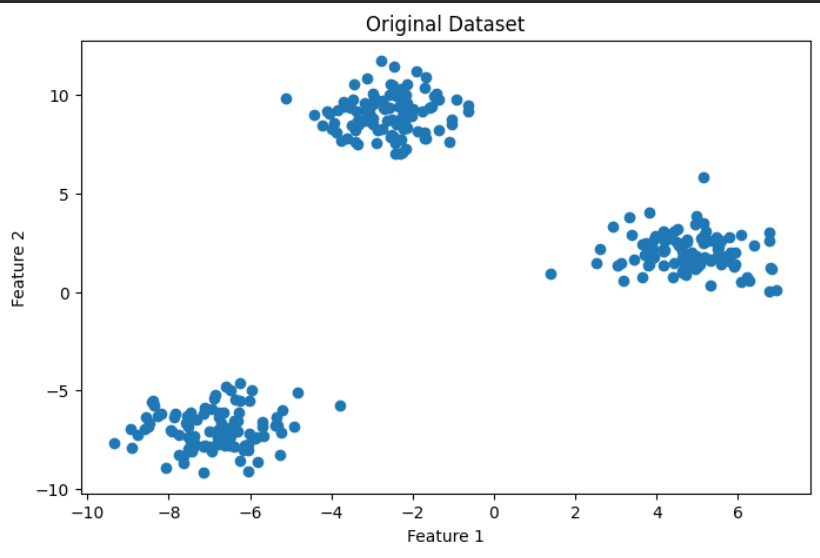
\includegraphics[width=0.75\linewidth]{km_dataset.png}
    \caption{Original Dataset (Before Clustering)}
    \label{fig:km_dataset}
\end{figure}

\begin{figure}[H]
    \centering
    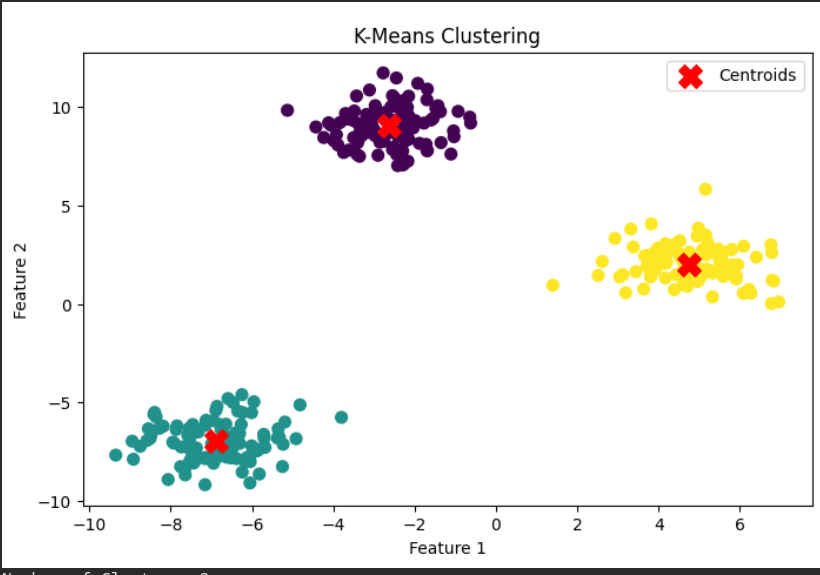
\includegraphics[width=0.75\linewidth]{km_output.png}
    \caption{K-Means Clustering Output with Centroids}
    \label{fig:km_output}
\end{figure}

\paragraph{Expected Result}
The K-Means algorithm successfully divides the dataset into three clusters based on the distance between data points and their centroids. The visualization shows three relatively distinct groups of data points, and the evaluation metrics confirm good cluster separation.

\subsubsection{Discussion \& Observations}

The K-Means algorithm successfully divided the dataset into three clusters. The obtained inertia value indicates how closely the data points are grouped around their respective cluster centroids. A lower inertia value indicates that the points are more compact within their clusters.

The silhouette score was used to evaluate the quality of the clustering. A value closer to 1 indicates that the clusters are well separated, while a value near 0 indicates overlapping clusters. In this experiment, the obtained silhouette score indicates that the generated clusters are reasonably well separated.

The \texttt{n\_init} parameter helps improve the stability of K-Means by running the algorithm multiple times with different centroid initializations and selecting the best result. Increasing \texttt{n\_init} can reduce the chance of obtaining a poor local solution. The \texttt{random\_state} parameter ensures that the experiment produces reproducible results.

Since the synthetic dataset was generated with three true groups, the clustering result can also be compared with the original labels. The predicted cluster numbers may differ from the true label numbers because cluster labels are arbitrary. For example, predicted cluster 0 may correspond to true cluster 2. Therefore, the comparison should focus on whether the same groups of data points have been identified rather than directly comparing the numerical labels.

\subsubsection{Conclusion \& Limitations}

In this experiment, K-Means clustering was successfully implemented to divide the dataset into three clusters. The cluster visualization, inertia, and silhouette score were used to evaluate the clustering performance. The results demonstrate that K-Means can effectively identify well-separated groups in the given dataset.

However, K-Means has several limitations. It is sensitive to the initial selection of centroids, although using multiple initializations with \texttt{n\_init} can reduce this problem. The algorithm also requires the number of clusters, $K$, to be specified before training. In addition, K-Means works best when clusters are approximately spherical and similar in size. It may perform poorly on datasets containing irregularly shaped, overlapping, or highly different-sized clusters.

Therefore, K-Means is simple and efficient for suitable datasets, but the choice of $K$, centroid initialization, and the structure of the dataset should be considered when applying the algorithm.

% ============================================================
% PROBLEM 2
% ============================================================
% ============================================================
% PROBLEM 2
% ============================================================
\subsection{Experiment 2: Modified K-Means Clustering}

\subsubsection{Objective}
The objective of this experiment is to implement a \textbf{Modified K-Means Clustering algorithm} with an improved method for selecting the initial centroids. Specifically, the experiment aims to:
\begin{itemize}
    \item Understand the limitations of random centroid initialization in standard K-Means.
    \item Select initial centroids using a \textbf{maximum-distance-based approach}.
    \item Apply K-Means clustering using the selected centroids.
    \item Visualize the resulting clusters.
    \item Compare the Modified K-Means result with standard K-Means.
\end{itemize}

\subsubsection{Suggested Dataset}
A \textbf{Synthetic Blob Dataset} generated using the \texttt{make\_blobs()} function from Scikit-learn is used. Its configuration is:

\begin{table}[H]
\centering
\caption{Synthetic Dataset Configuration}
\begin{tabular}{ll}
\toprule
\textbf{Property} & \textbf{Value} \\
\midrule
Number of samples            & 300 \\
Number of clusters (centers) & 3 \\
Number of features           & 2 \\
Cluster standard deviation   & 1.0 \\
Random state                 & 42 \\
\bottomrule
\end{tabular}
\end{table}

This dataset is suitable because the generated clusters can easily be visualized in two dimensions.

\subsubsection{Required Libraries}
\begin{itemize}
    \item \textbf{NumPy} -- for numerical operations.
    \item \textbf{Matplotlib} -- for data visualization.
    \item \textbf{Scikit-learn} -- for K-Means implementation, dataset generation, and evaluation.
\end{itemize}

\begin{lstlisting}[language=Python, caption={Required Imports}]
import numpy as np
import matplotlib.pyplot as plt

from sklearn.datasets import make_blobs
from sklearn.cluster import KMeans
from sklearn.metrics import silhouette_score
\end{lstlisting}

\subsubsection{Brief Theory}
Modified K-Means is an improved version of the standard K-Means algorithm where the \textbf{initial centroids are selected using a more systematic approach} instead of selecting them randomly. In standard K-Means, poor initial centroids can sometimes lead to poor clustering results.

The Modified K-Means approach used in this experiment selects initial centroids based on the \textbf{maximum distance between data points}.

\paragraph{Initial Centroid Selection}
For example, when $K = 2$, the two points having a large distance from each other can be selected as the initial centroids. For $K = 3$, after selecting the first two centroids, another point can be selected based on its distance from the already selected centroids. The general idea is to select initial centroids that are \textbf{far apart from each other}.

\paragraph{K-Means Steps}
After selecting the initial centroids, the normal K-Means process is performed:
\begin{enumerate}
    \item Select initial centroids.
    \item Calculate the distance between each data point and each centroid.
    \item Assign each point to the nearest centroid.
    \item Calculate new centroids.
    \item Repeat until the centroids become stable.
\end{enumerate}

\paragraph{Advantage}
The main purpose of this modification is to provide \textbf{better initial centroids}, which can make the clustering more stable and reduce the possibility of getting a poor local solution.

\subsubsection{Procedure}
\begin{enumerate}
    \item Import the required libraries.
    \item Generate the synthetic dataset.
    \item Visualize the original dataset.
    \item Select the required number of clusters, $K$.
    \item Select the first centroid.
    \item Calculate distances between data points and selected centroids.
    \item Select the next centroid from the points having the largest minimum distance.
    \item Repeat until $K$ initial centroids are selected.
    \item Use these centroids as the initial centroids of K-Means.
    \item Perform the K-Means clustering process.
    \item Visualize the final clusters and centroids.
    \item Calculate the inertia.
    \item Calculate the silhouette score.
    \item Compare the result with standard K-Means.
\end{enumerate}

\subsubsection{Reference Implementation}
\begin{lstlisting}[language=Python, caption={Modified K-Means Clustering Implementation}]
# ==========================================
# Experiment 2: Modified K-Means Clustering
# ==========================================

import numpy as np
import matplotlib.pyplot as plt

from sklearn.datasets import make_blobs
from sklearn.cluster import KMeans
from sklearn.metrics import silhouette_score

# 1. Generate dataset
X, y = make_blobs(
    n_samples=300,
    centers=3,
    cluster_std=1.0,
    random_state=42
)

# 2. Visualize original dataset
plt.figure(figsize=(8, 5))
plt.scatter(X[:, 0], X[:, 1])
plt.title("Original Dataset")
plt.xlabel("Feature 1")
plt.ylabel("Feature 2")
plt.show()

# ==========================================
# 3. Modified Centroid Initialization
# ==========================================
def modified_initialization(X, k):
    # Select the first centroid
    centroids = [X[0]]
    for _ in range(1, k):
        # Calculate distance of every point
        # from the nearest selected centroid
        distances = np.array([
            min(np.linalg.norm(x - c) for c in centroids)
            for x in X
        ])
        # Select the point with maximum distance
        next_centroid = X[np.argmax(distances)]
        centroids.append(next_centroid)
    return np.array(centroids)

# 4. Set number of clusters
k = 3

# 5. Select initial centroids using
#    Modified K-Means method
initial_centroids = modified_initialization(X, k)

print("Initial Centroids:")
print(initial_centroids)

# ==========================================
# 6. Apply K-Means using selected centroids
# ==========================================
kmeans_modified = KMeans(
    n_clusters=k,
    init=initial_centroids,
    n_init=1,
    random_state=42
)
labels = kmeans_modified.fit_predict(X)

# 7. Get final centroids
final_centroids = kmeans_modified.cluster_centers_

# ==========================================
# 8. Visualize Modified K-Means Clusters
# ==========================================
plt.figure(figsize=(8, 5))
plt.scatter(X[:, 0], X[:, 1], c=labels, cmap="viridis", s=50)
plt.scatter(
    final_centroids[:, 0],
    final_centroids[:, 1],
    marker="X",
    s=200,
    color="red",
    label="Final Centroids"
)
plt.title("Modified K-Means Clustering")
plt.xlabel("Feature 1")
plt.ylabel("Feature 2")
plt.legend()
plt.show()

# ==========================================
# 9. Evaluation
# ==========================================
inertia = kmeans_modified.inertia_
silhouette = silhouette_score(X, labels)

print("\nEvaluation Results")
print("-------------------------")
print("Number of Clusters:", k)
print("Inertia:", inertia)
print("Silhouette Score:", silhouette)

# 10. Cluster sizes
for i in range(k):
    print(f"Cluster {i}: {np.sum(labels == i)} data points")
\end{lstlisting}

\subsubsection{Evaluation / Expected Output}

\paragraph{Output}
After running the program, two plots are produced:
\begin{itemize}
    \item A scatter plot of the original dataset before clustering.
    \item A scatter plot of the Modified K-Means clustering result showing three differently colored clusters with red \texttt{X} marks representing the final cluster centroids.
\end{itemize}
The console also prints the initial centroids, evaluation metrics, and the number of data points in each cluster.

\begin{table}[H]
\centering
\caption{Hyperparameters \& Results for Modified K-Means}
\begin{tabular}{ll}
\toprule
\textbf{Parameter / Metric} & \textbf{Value} \\
\midrule
Number of Clusters ($K$)        & 3 \\
Initialization Method           & Maximum-Distance-Based \\
Number of Initializations       & 1 \\
Random State                    & 42 \\
Inertia                         & \textit{(fill in)} \\
Silhouette Score                & \textit{(fill in)} \\
\bottomrule
\end{tabular}
\end{table}

\begin{table}[H]
\centering
\caption{Cluster Distribution}
\begin{tabular}{lc}
\toprule
\textbf{Cluster} & \textbf{Number of Data Points} \\
\midrule
Cluster 0 & \textit{(fill in)} \\
Cluster 1 & \textit{(fill in)} \\
Cluster 2 & \textit{(fill in)} \\
\bottomrule
\end{tabular}
\end{table}

\begin{figure}[H]
    \centering
    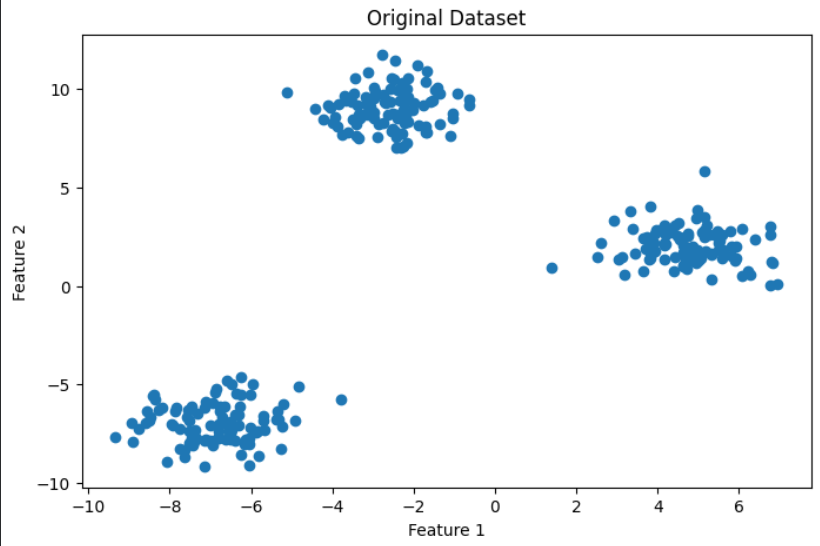
\includegraphics[width=0.75\linewidth]{mkm_dataset.png}
    \caption{Original Dataset (Before Clustering)}
    \label{fig:mkm_dataset}
\end{figure}

\begin{figure}[H]
    \centering
    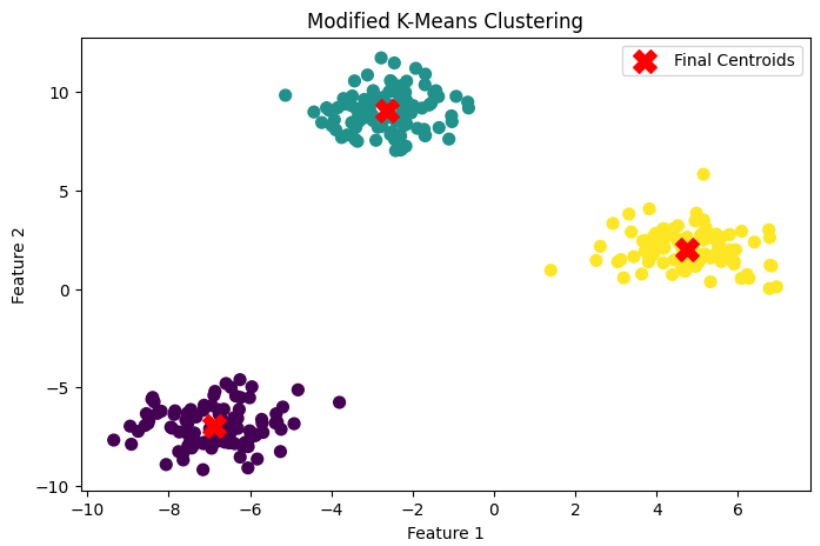
\includegraphics[width=0.75\linewidth]{mkm_output.png}
    \caption{Modified K-Means Clustering Output with Final Centroids}
    \label{fig:mkm_output}
\end{figure}

\paragraph{Expected Result}
The Modified K-Means algorithm successfully divides the dataset into three clusters using a maximum-distance-based centroid initialization method. The visualization shows three relatively distinct groups of data points, and the evaluation metrics confirm good cluster separation.

\subsubsection{Discussion \& Observations}

The Modified K-Means algorithm successfully divided the dataset into three clusters using a maximum-distance-based centroid initialization method. Instead of relying on random initialization, the method selects initial centroids that are relatively far apart from each other.

The selected initial centroids provide a better starting point for the K-Means optimization process. The resulting inertia and silhouette score can be used to evaluate the compactness and separation of the generated clusters.

The Modified K-Means result can also be compared with the standard K-Means result. Differences in inertia or silhouette score may occur because the two methods start with different initial centroids. Since cluster labels are arbitrary, the numerical cluster labels should not be directly compared with the original labels.

The method is particularly useful when poor random initialization causes standard K-Means to converge to an undesirable solution.

\subsubsection{Conclusion \& Limitations}

In this experiment, a Modified K-Means algorithm was implemented using a maximum-distance-based method for selecting initial centroids. The selected centroids were then used as the starting points for the standard K-Means clustering process. The results show that systematic centroid initialization can provide a more controlled starting point than random initialization.

However, the Modified K-Means algorithm still has some limitations. The number of clusters, $K$, must be specified in advance. The method can also be affected by outliers because extreme data points may be selected as centroids. In addition, the algorithm still assumes that the clusters are relatively compact and spherical. The modified initialization improves the starting point but does not remove the fundamental limitations of K-Means.
% SPACE FOR PROBLEM 2

% ============================================================
% PROBLEM 3
% ============================================================
% ============================================================
% PROBLEM 3
% ============================================================
\subsection{Experiment 3: Hierarchical Clustering}

\subsubsection{Objective}
The objective of this experiment is to implement the Hierarchical Clustering algorithm to group similar data points into clusters. Specifically, the experiment aims to:
\begin{itemize}
    \item Understand how hierarchical clustering works.
    \item Learn the difference between Agglomerative and Divisive clustering.
    \item Apply Agglomerative Hierarchical Clustering.
    \item Visualize clusters using a dendrogram.
    \item Evaluate clustering performance using Silhouette Score.
\end{itemize}

\subsubsection{Suggested Dataset}
A \textbf{Synthetic Blob Dataset} generated using the \texttt{make\_blobs()} function from Scikit-learn is used. Its configuration is:

\begin{table}[H]
\centering
\caption{Synthetic Dataset Configuration}
\begin{tabular}{ll}
\toprule
\textbf{Property} & \textbf{Value} \\
\midrule
Number of samples            & 100 \\
Number of clusters (centers) & 3 \\
Number of features           & 2 \\
Cluster standard deviation   & 1.0 \\
Random state                 & 42 \\
\bottomrule
\end{tabular}
\end{table}

This dataset is suitable because it contains two-dimensional data points that can easily be visualized.

\subsubsection{Required Libraries}
\begin{itemize}
    \item \textbf{NumPy} -- for numerical operations.
    \item \textbf{Matplotlib} -- for visualization.
    \item \textbf{Scikit-learn} -- for clustering and evaluation.
    \item \textbf{SciPy} -- for generating the dendrogram.
\end{itemize}

\begin{lstlisting}[language=Python, caption={Required Imports}]
import numpy as np
import matplotlib.pyplot as plt

from sklearn.datasets import make_blobs
from sklearn.cluster import AgglomerativeClustering
from sklearn.metrics import silhouette_score

from scipy.cluster.hierarchy import dendrogram, linkage
\end{lstlisting}

\subsubsection{Brief Theory}
Hierarchical Clustering is an unsupervised machine learning algorithm used to group similar data points into a hierarchy of clusters. Unlike K-Means, it does not require selecting the number of clusters at the beginning. The number of clusters can be selected later by cutting the dendrogram at a particular level.

\paragraph{Types of Hierarchical Clustering}
\begin{enumerate}
    \item \textbf{Agglomerative Clustering (Bottom-Up):} Initially, every data point is treated as a separate cluster. The two closest clusters are merged. This process continues until all points belong to one cluster or the desired number of clusters is reached.
    \item \textbf{Divisive Clustering (Top-Down):} Initially, all data points belong to one cluster. The cluster is gradually divided into smaller clusters. This process continues until the required number of clusters is obtained.
\end{enumerate}
In this experiment, we use Agglomerative Hierarchical Clustering.

\paragraph{Linkage Methods}
Linkage determines how the distance between two clusters is calculated:
\begin{itemize}
    \item \textbf{Single Linkage:} Uses the minimum distance between two clusters.
    \item \textbf{Complete Linkage:} Uses the maximum distance between two clusters.
    \item \textbf{Average Linkage:} Uses the average distance between all points in two clusters.
    \item \textbf{Ward Linkage:} Merges clusters that result in the smallest increase in within-cluster variance.
\end{itemize}

\paragraph{Dendrogram}
A dendrogram is a tree-like diagram that shows how clusters are merged at different distances. It helps determine the suitable number of clusters by cutting the dendrogram at a selected height.

\paragraph{Distance Calculation}
Euclidean distance is commonly used to measure the distance between two data points:
\[
d(x, y) = \sqrt{\sum_{i=1}^{n}(x_i - y_i)^2}
\]

\paragraph{Evaluation Metric}
\textbf{Silhouette Score:} Measures how well-separated the clusters are.
\begin{itemize}
    \item Close to $1$: Well-separated clusters.
    \item Close to $0$: Overlapping clusters.
    \item Negative: Possible incorrect clustering.
\end{itemize}

\subsubsection{Procedure}
\begin{enumerate}
    \item Import the required Python libraries.
    \item Generate the synthetic dataset using \texttt{make\_blobs()}.
    \item Visualize the original dataset.
    \item Calculate the hierarchical linkage using the Ward method.
    \item Generate a dendrogram to visualize the cluster merging process.
    \item Select the number of clusters, $K = 3$.
    \item Apply Agglomerative Hierarchical Clustering.
    \item Assign each data point to its respective cluster.
    \item Visualize the final clusters.
    \item Calculate the Silhouette Score.
    \item Display the number of data points in each cluster.
    \item Analyze the clustering results.
\end{enumerate}

\subsubsection{Reference Implementation}
\begin{lstlisting}[language=Python, caption={Hierarchical Clustering Implementation}]
# ==========================================
# Experiment 3: Hierarchical Clustering
# ==========================================

# 1. Import required libraries
import numpy as np
import matplotlib.pyplot as plt

from sklearn.datasets import make_blobs
from sklearn.cluster import AgglomerativeClustering
from sklearn.metrics import silhouette_score

from scipy.cluster.hierarchy import dendrogram, linkage

# 2. Generate synthetic dataset
X, y = make_blobs(
    n_samples=100,
    centers=3,
    cluster_std=1.0,
    random_state=42
)

# 3. Visualize original dataset
plt.figure(figsize=(8, 5))
plt.scatter(X[:, 0], X[:, 1])
plt.title("Original Dataset")
plt.xlabel("Feature 1")
plt.ylabel("Feature 2")
plt.show()

# ==========================================
# 4. Generate Dendrogram
# ==========================================
# Apply Ward linkage
Z = linkage(X, method='ward')

plt.figure(figsize=(12, 6))
dendrogram(
    Z,
    truncate_mode='lastp',
    p=30
)
plt.title("Hierarchical Clustering Dendrogram")
plt.xlabel("Data Points / Clusters")
plt.ylabel("Euclidean Distance")
plt.show()

# ==========================================
# 5. Apply Agglomerative Clustering
# ==========================================
k = 3
hc = AgglomerativeClustering(
    n_clusters=k,
    linkage='ward'
)
labels = hc.fit_predict(X)

# ==========================================
# 6. Visualize Final Clusters
# ==========================================
plt.figure(figsize=(8, 5))
plt.scatter(X[:, 0], X[:, 1], c=labels, cmap='viridis', s=50)
plt.title("Agglomerative Hierarchical Clustering")
plt.xlabel("Feature 1")
plt.ylabel("Feature 2")
plt.show()

# ==========================================
# 7. Evaluation
# ==========================================
silhouette = silhouette_score(X, labels)

print("Evaluation Results")
print("-------------------------")
print("Number of Clusters:", k)
print("Silhouette Score:", silhouette)

# ==========================================
# 8. Display Cluster Information
# ==========================================
for i in range(k):
    print(f"Cluster {i}: {np.sum(labels == i)} data points")
\end{lstlisting}

\subsubsection{Evaluation / Expected Output}

\paragraph{Output}
After running the program, three plots are produced:
\begin{itemize}
    \item A scatter plot of the original dataset before clustering.
    \item A dendrogram showing how individual data points are merged into larger clusters.
    \item A scatter plot of the Agglomerative Hierarchical Clustering result showing three differently colored clusters.
\end{itemize}
The console also prints the evaluation metrics and the number of data points in each cluster.

\begin{table}[H]
\centering
\caption{Hyperparameters \& Results for Hierarchical Clustering}
\begin{tabular}{ll}
\toprule
\textbf{Parameter / Metric} & \textbf{Value} \\
\midrule
Number of Clusters ($K$) & 3 \\
Linkage Method           & Ward \\
Distance Metric          & Euclidean \\
Random State             & 42 \\
Silhouette Score         & \textit{(fill in)} \\
\bottomrule
\end{tabular}
\end{table}

\begin{table}[H]
\centering
\caption{Cluster Distribution}
\begin{tabular}{lc}
\toprule
\textbf{Cluster} & \textbf{Number of Data Points} \\
\midrule
Cluster 0 & \textit{(fill in)} \\
Cluster 1 & \textit{(fill in)} \\
Cluster 2 & \textit{(fill in)} \\
\bottomrule
\end{tabular}
\end{table}

\begin{figure}[H]
    \centering
    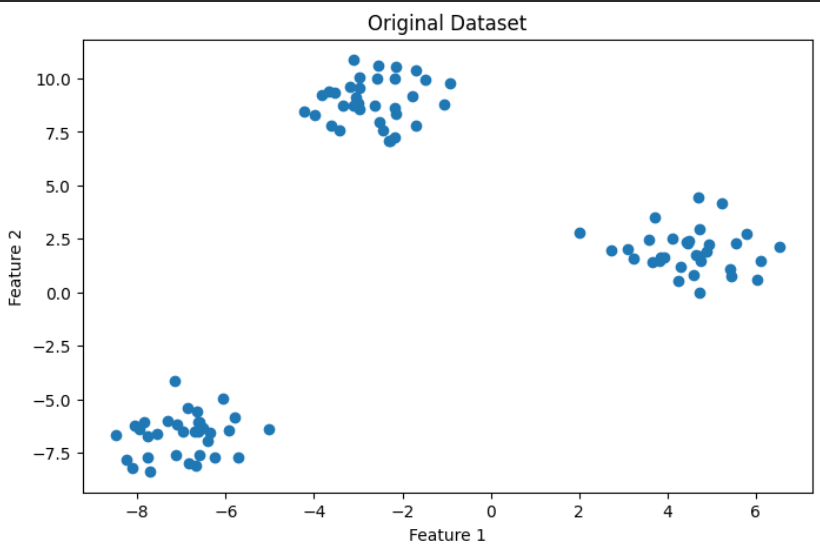
\includegraphics[width=0.75\linewidth]{hc_dataset.png}
    \caption{Original Dataset (Before Clustering)}
    \label{fig:hc_dataset}
\end{figure}

\begin{figure}[H]
    \centering
    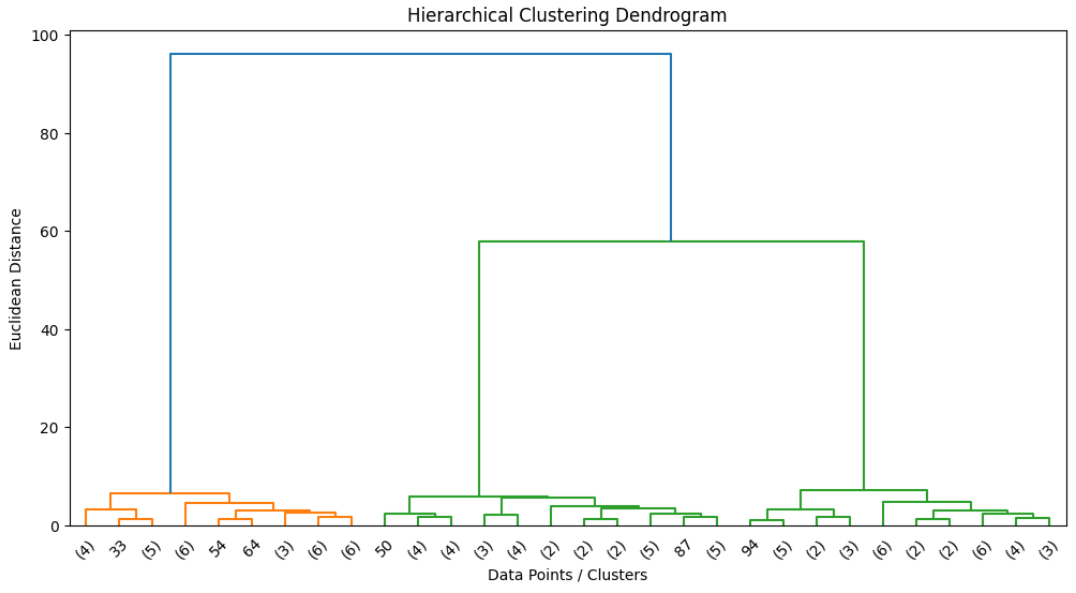
\includegraphics[width=0.85\linewidth]{hc_dendrogram.png}
    \caption{Hierarchical Clustering Dendrogram}
    \label{fig:hc_dendrogram}
\end{figure}

\begin{figure}[H]
    \centering
    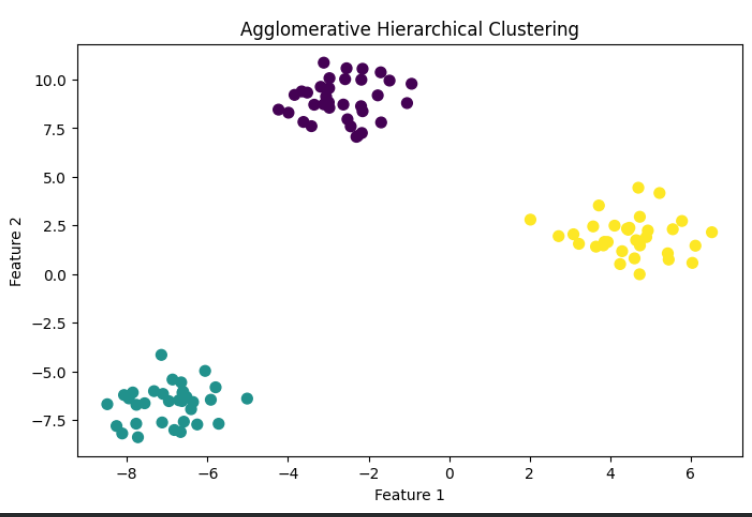
\includegraphics[width=0.75\linewidth]{hc_output.png}
    \caption{Agglomerative Hierarchical Clustering Output}
    \label{fig:hc_output}
\end{figure}

\paragraph{Expected Result}
The Hierarchical Clustering algorithm successfully groups the dataset into three clusters using the Agglomerative approach. The dendrogram visually represents the merging process, and the evaluation metrics confirm good cluster separation.

\subsubsection{Discussion \& Observations}

The Hierarchical Clustering algorithm successfully grouped the dataset into three clusters using the Agglomerative approach. Initially, each data point was considered a separate cluster. The algorithm gradually merged the closest clusters based on the Ward linkage method.

The dendrogram visually represents the merging process and helps understand the hierarchical relationship between clusters. By observing the dendrogram, the number of clusters can be selected by cutting it at an appropriate distance.

The Silhouette Score was used to evaluate the clustering performance. A score closer to 1 indicates better-separated clusters, while a score near 0 indicates overlapping clusters.

The Ward linkage method generally produces compact clusters by minimizing the increase in within-cluster variance during merging.

Unlike K-Means, Hierarchical Clustering does not require specifying the number of clusters during the dendrogram generation process. However, the number of clusters must be specified when applying the final Agglomerative Clustering model.

\subsubsection{Conclusion \& Limitations}

In this experiment, Agglomerative Hierarchical Clustering was successfully implemented using the Ward linkage method. The algorithm grouped similar data points into three clusters, and the dendrogram provided a visual representation of the cluster merging process.

The experiment demonstrates that Hierarchical Clustering is useful for understanding relationships among data points and identifying natural group structures.

However, Hierarchical Clustering has some limitations. It can be computationally expensive for large datasets because it requires calculating distances between data points or clusters. The algorithm is also sensitive to the choice of linkage method and distance metric. Once two clusters are merged, the decision cannot be reversed. Additionally, outliers may affect the clustering results.
% ============================================================
% PROBLEM 4
% ============================================================
% ============================================================
% PROBLEM 4
% ============================================================
\subsection{Experiment 4: Fuzzy C-Means Clustering}

\subsubsection{Objective}
The objective of this experiment is to implement the Fuzzy C-Means (FCM) Clustering algorithm to group similar data points into different clusters. Specifically, the experiment aims to:
\begin{itemize}
    \item Understand the concept of fuzzy clustering.
    \item Learn how Fuzzy C-Means differs from K-Means.
    \item Assign membership values to data points instead of assigning them to only one cluster.
    \item Calculate cluster centers using membership values.
    \item Visualize the resulting clusters.
    \item Evaluate clustering performance using the Silhouette Score.
\end{itemize}

\subsubsection{Suggested Dataset}
A \textbf{Synthetic Blob Dataset} generated using the \texttt{make\_blobs()} function from Scikit-learn is used. Its configuration is:

\begin{table}[H]
\centering
\caption{Synthetic Dataset Configuration}
\begin{tabular}{ll}
\toprule
\textbf{Property} & \textbf{Value} \\
\midrule
Number of samples            & 300 \\
Number of clusters (centers) & 3 \\
Number of features           & 2 \\
Cluster standard deviation   & 1.0 \\
Random state                 & 42 \\
\bottomrule
\end{tabular}
\end{table}

This dataset is suitable because it contains two-dimensional data points that can easily be visualized.

\subsubsection{Required Libraries}
\begin{itemize}
    \item \textbf{NumPy} -- for numerical calculations.
    \item \textbf{Matplotlib} -- for data visualization.
    \item \textbf{Scikit-learn} -- for dataset generation and evaluation.
    \item \textbf{scikit-fuzzy} -- for implementing Fuzzy C-Means clustering.
\end{itemize}

Install the required package in Google Colab:
\begin{lstlisting}[language=Python, caption={Install scikit-fuzzy}]
!pip install scikit-fuzzy
\end{lstlisting}

\begin{lstlisting}[language=Python, caption={Required Imports}]
import numpy as np
import matplotlib.pyplot as plt

import skfuzzy as fuzz

from sklearn.datasets import make_blobs
from sklearn.metrics import silhouette_score
\end{lstlisting}

\subsubsection{Brief Theory}
Fuzzy C-Means (FCM) is an unsupervised machine learning algorithm that divides data into multiple clusters based on their similarity. Unlike K-Means, FCM allows a data point to belong to more than one cluster with different membership values.

For example, a data point may have 70\% membership in Cluster 1, 20\% in Cluster 2, and 10\% in Cluster 3. The sum of membership values for each data point is always equal to 1.

\paragraph{Membership Function}
\[
\sum_{j=1}^{C} u_{ij} = 1
\]
where $u_{ij}$ is the membership value of data point $i$ in cluster $j$, and $C$ is the number of clusters.

\paragraph{Cluster Center Calculation}
\[
v_j = \frac{\sum_{i=1}^{N} u_{ij}^{m} x_i}{\sum_{i=1}^{N} u_{ij}^{m}}
\]
where $v_j$ is the center of cluster $j$, $x_i$ is a data point, $u_{ij}$ is the membership value, $m$ is the fuzziness parameter, and $N$ is the total number of data points.

\paragraph{Fuzziness Parameter ($m$)}
The fuzziness parameter controls how softly data points are assigned to clusters:
\begin{itemize}
    \item When $m$ is close to 1, the clustering becomes harder.
    \item A larger $m$ produces softer membership assignments.
    \item The commonly used value is $m = 2$.
\end{itemize}

\paragraph{Objective Function}
\[
J_m = \sum_{i=1}^{N} \sum_{j=1}^{C} u_{ij}^{m} \| x_i - v_j \|^2
\]
The algorithm repeatedly updates membership values and cluster centers until convergence.

\paragraph{Difference Between K-Means and Fuzzy C-Means}
\begin{table}[H]
\centering
\caption{K-Means vs.\ Fuzzy C-Means}
\begin{tabular}{ll}
\toprule
\textbf{K-Means} & \textbf{Fuzzy C-Means} \\
\midrule
Hard clustering                     & Soft clustering \\
One point belongs to one cluster    & One point can belong to multiple clusters \\
Uses centroid-based assignment      & Uses membership values \\
Does not use a fuzziness parameter  & Uses fuzziness parameter $m$ \\
\bottomrule
\end{tabular}
\end{table}

\paragraph{Evaluation Metric}
\textbf{Silhouette Score:} Measures how well-separated the clusters are.
\begin{itemize}
    \item Close to $1$: Well-separated clusters.
    \item Close to $0$: Overlapping clusters.
    \item Negative: Possible incorrect clustering.
\end{itemize}
For FCM, the membership values can be converted into hard labels by assigning each point to the cluster where it has the highest membership.

\subsubsection{Procedure}
\begin{enumerate}
    \item Import the required Python libraries.
    \item Install and import the \texttt{scikit-fuzzy} library.
    \item Generate the synthetic dataset using \texttt{make\_blobs()}.
    \item Visualize the original dataset.
    \item Set the number of clusters, $C = 3$.
    \item Set the fuzziness parameter, $m = 2$.
    \item Convert the dataset into the required format for Fuzzy C-Means.
    \item Apply the Fuzzy C-Means algorithm.
    \item Calculate the membership values for each data point.
    \item Calculate the final cluster centers.
    \item Assign each data point to the cluster with the highest membership value.
    \item Visualize the final clusters and cluster centers.
    \item Calculate the Silhouette Score.
    \item Display the membership values and number of data points in each cluster.
    \item Analyze the clustering results.
\end{enumerate}

\subsubsection{Reference Implementation}
\begin{lstlisting}[language=Python, caption={Fuzzy C-Means Clustering Implementation}]
# ==========================================
# Experiment 4: Fuzzy C-Means Clustering
# ==========================================

# 1. Import required libraries
import numpy as np
import matplotlib.pyplot as plt

import skfuzzy as fuzz

from sklearn.datasets import make_blobs
from sklearn.metrics import silhouette_score

# 2. Generate synthetic dataset
X, y = make_blobs(
    n_samples=300,
    centers=3,
    cluster_std=1.0,
    random_state=42
)

# 3. Visualize original dataset
plt.figure(figsize=(8, 5))
plt.scatter(X[:, 0], X[:, 1])
plt.title("Original Dataset")
plt.xlabel("Feature 1")
plt.ylabel("Feature 2")
plt.show()

# ==========================================
# 4. Set FCM Parameters
# ==========================================
c = 3
m = 2.0

# 5. Convert data into required format
# FCM expects features x samples
data = X.T

# ==========================================
# 6. Apply Fuzzy C-Means
# ==========================================
centers, membership, initial_membership, \
distance, objective, iterations, fpc = fuzz.cluster.cmeans(
    data,
    c=c,
    m=m,
    error=0.005,
    maxiter=1000,
    init=None,
    seed=42
)

# ==========================================
# 7. Get Cluster Labels
# ==========================================
# Assign each point to the cluster
# with the highest membership value
labels = np.argmax(membership, axis=0)

# ==========================================
# 8. Visualize Final Clusters
# ==========================================
plt.figure(figsize=(8, 5))
plt.scatter(X[:, 0], X[:, 1], c=labels, cmap='viridis', s=50)
plt.scatter(
    centers[:, 0],
    centers[:, 1],
    marker='X',
    s=200,
    color='red',
    label='Cluster Centers'
)
plt.title("Fuzzy C-Means Clustering")
plt.xlabel("Feature 1")
plt.ylabel("Feature 2")
plt.legend()
plt.show()

# ==========================================
# 9. Display Membership Values
# ==========================================
print("Membership Values (First 5 Data Points):")
print(membership[:, :5])

# ==========================================
# 10. Evaluation
# ==========================================
silhouette = silhouette_score(X, labels)

print("\nEvaluation Results")
print("-------------------------")
print("Number of Clusters:", c)
print("Fuzziness Parameter:", m)
print("Silhouette Score:", silhouette)
print("Fuzzy Partition Coefficient:", fpc)
print("Number of Iterations:", iterations)

# ==========================================
# 11. Display Cluster Information
# ==========================================
for i in range(c):
    print(f"Cluster {i}: {np.sum(labels == i)} data points")
\end{lstlisting}

\subsubsection{Evaluation / Expected Output}

\paragraph{Output}
After running the program, two plots are produced:
\begin{itemize}
    \item A scatter plot of the original dataset before clustering.
    \item A scatter plot of the Fuzzy C-Means clustering result showing three differently colored clusters with red \texttt{X} marks representing the final cluster centers.
\end{itemize}
The console also prints the membership values for the first five data points, the evaluation metrics, and the number of data points in each cluster.

\begin{table}[H]
\centering
\caption{Hyperparameters \& Results for Fuzzy C-Means}
\begin{tabular}{ll}
\toprule
\textbf{Parameter / Metric} & \textbf{Value} \\
\midrule
Number of Clusters ($C$)             & 3 \\
Fuzziness Parameter ($m$)            & 2.0 \\
Maximum Iterations                   & 1000 \\
Convergence Error Tolerance          & 0.005 \\
Seed                                 & 42 \\
Silhouette Score                     & \textit{(fill in)} \\
Fuzzy Partition Coefficient (FPC)    & \textit{(fill in)} \\
Number of Iterations                 & \textit{(fill in)} \\
\bottomrule
\end{tabular}
\end{table}

\begin{table}[H]
\centering
\caption{Cluster Distribution}
\begin{tabular}{lc}
\toprule
\textbf{Cluster} & \textbf{Number of Data Points} \\
\midrule
Cluster 0 & \textit{(fill in)} \\
Cluster 1 & \textit{(fill in)} \\
Cluster 2 & \textit{(fill in)} \\
\bottomrule
\end{tabular}
\end{table}

\begin{figure}[H]
    \centering
    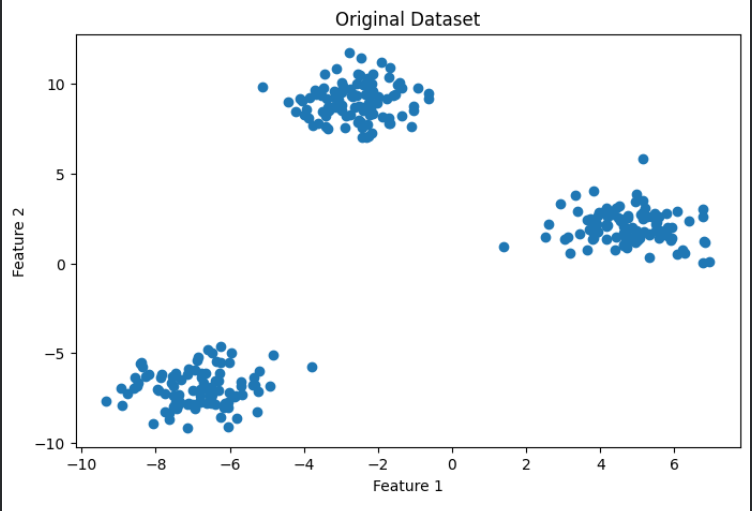
\includegraphics[width=0.75\linewidth]{fcm_dataset.png}
    \caption{Original Dataset (Before Clustering)}
    \label{fig:fcm_dataset}
\end{figure}

\begin{figure}[H]
    \centering
    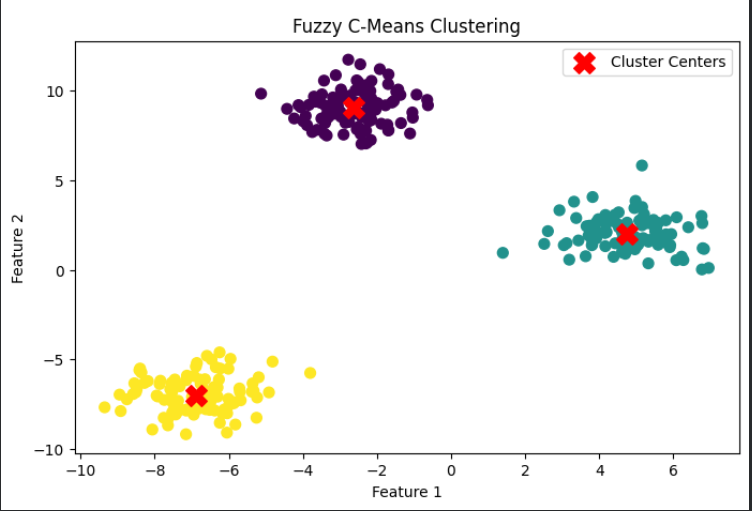
\includegraphics[width=0.75\linewidth]{fcm_output.png}
    \caption{Fuzzy C-Means Clustering Output with Cluster Centers}
    \label{fig:fcm_output}
\end{figure}

\paragraph{Expected Result}
The Fuzzy C-Means algorithm successfully divides the dataset into three clusters using fuzzy membership values. The visualization shows three relatively distinct groups of data points, and the evaluation metrics confirm good cluster separation.

\subsubsection{Discussion \& Observations}

The Fuzzy C-Means algorithm successfully divided the dataset into three clusters using fuzzy membership values. Unlike K-Means, each data point was assigned a membership value for every cluster rather than belonging to only one cluster.

The membership values indicate the degree to which each data point belongs to different clusters. Data points near the center of a cluster generally have higher membership values for that cluster, while points near the boundaries may have more balanced membership values.

The cluster centers were calculated using the membership values and the fuzziness parameter. The Fuzzy Partition Coefficient (FPC) was used to evaluate the clarity of the fuzzy partition, while the Silhouette Score measured cluster separation after converting membership values into hard labels.

The fuzziness parameter, $m = 2$, controlled the softness of the membership assignments. A higher value of $m$ generally produces more distributed membership values.

Overall, the experiment demonstrates that Fuzzy C-Means provides more flexible clustering than K-Means, especially when data points may belong to multiple clusters.

\subsubsection{Conclusion \& Limitations}

In this experiment, the Fuzzy C-Means Clustering algorithm was successfully implemented to group the dataset into three clusters. The algorithm calculated fuzzy membership values and cluster centers using an iterative optimization process.

The experiment demonstrated that Fuzzy C-Means allows data points to have different degrees of membership in multiple clusters, making it useful for handling overlapping data.

However, Fuzzy C-Means has several limitations. It requires the number of clusters to be specified in advance. The algorithm is sensitive to initial membership values and the fuzziness parameter. It can also be computationally expensive for large datasets because membership values are repeatedly updated. Additionally, it is sensitive to outliers and generally works better with compact clusters.

Therefore, Fuzzy C-Means is useful when cluster boundaries are unclear and soft membership assignments are more appropriate than hard clustering.



% ============================================================
% DENSITY-BASED LEARNING
% ============================================================
\section{Density-Based Learning}

% ------------------------------------------------------------
% EXPERIMENT 5
% ------------------------------------------------------------
\subsection{Experiment 5: DBSCAN Clustering}

\subsubsection{Objective}
The objective of this experiment is to implement the DBSCAN (Density-Based Spatial Clustering of Applications with Noise) algorithm to identify clusters based on the density of data points. Specifically, the experiment aims to:
\begin{itemize}
    \item Understand density-based clustering.
    \item Identify dense regions in a dataset.
    \item Detect noise and outliers.
    \item Apply DBSCAN using different parameters.
    \item Visualize the resulting clusters.
    \item Evaluate clustering performance using Silhouette Score.
\end{itemize}

\subsubsection{Suggested Dataset}
A \textbf{Synthetic Moon Dataset} generated using the \texttt{make\_moons()} function from Scikit-learn is used. Its configuration is:

\begin{table}[H]
\centering
\caption{Synthetic Dataset Configuration}
\begin{tabular}{ll}
\toprule
\textbf{Property} & \textbf{Value} \\
\midrule
Number of samples  & 300 \\
Noise              & 0.08 \\
Number of features & 2 \\
Random state       & 42 \\
\bottomrule
\end{tabular}
\end{table}

This dataset is suitable because it contains non-spherical, curved clusters that demonstrate the advantage of density-based clustering over K-Means.

\subsubsection{Required Libraries}
\begin{itemize}
    \item \textbf{NumPy} -- for numerical operations.
    \item \textbf{Matplotlib} -- for visualization.
    \item \textbf{Scikit-learn} -- for dataset generation, DBSCAN, and evaluation.
\end{itemize}

\begin{lstlisting}[language=Python, caption={Required Imports}]
import numpy as np
import matplotlib.pyplot as plt

from sklearn.datasets import make_moons
from sklearn.cluster import DBSCAN
from sklearn.metrics import silhouette_score
\end{lstlisting}

\subsubsection{Brief Theory}
DBSCAN is an unsupervised machine learning algorithm that groups data points based on their density. Unlike K-Means, DBSCAN does not require specifying the number of clusters in advance and can identify noise and outliers.

\paragraph{Important Parameters}
\begin{enumerate}
    \item \textbf{Epsilon (\texttt{eps}):} The maximum distance between two points for them to be considered neighbors. A smaller epsilon may create many small clusters, while a larger epsilon may merge different clusters.
    \item \textbf{Minimum Samples (\texttt{min\_samples}):} The minimum number of neighboring points required to form a dense region.
\end{enumerate}

\paragraph{Types of Points}
DBSCAN identifies three types of points:
\begin{itemize}
    \item \textbf{Core Point:} A point having at least \texttt{min\_samples} points within its epsilon neighborhood.
    \item \textbf{Border Point:} A point that is not a core point but lies within the neighborhood of a core point.
    \item \textbf{Noise Point:} A point that does not belong to any cluster.
\end{itemize}

\paragraph{Main Steps}
\begin{enumerate}
    \item Select a data point.
    \item Find its neighboring points within epsilon distance.
    \item Check whether it is a core point.
    \item Expand the cluster using density-connected points.
    \item Mark points that do not belong to any cluster as noise.
    \item Continue until all points are processed.
\end{enumerate}

\paragraph{Distance Calculation}
DBSCAN commonly uses Euclidean distance:
\[
d(x, y) = \sqrt{\sum_{i=1}^{n}(x_i - y_i)^2}
\]

\paragraph{Evaluation Metric}
\textbf{Silhouette Score:} Measures cluster separation. Noise points are excluded when calculating the score in this experiment because they are not assigned to regular clusters.

\subsubsection{Procedure}
\begin{enumerate}
    \item Import the required Python libraries.
    \item Generate the Synthetic Moon Dataset using \texttt{make\_moons()}.
    \item Visualize the original dataset.
    \item Set the DBSCAN parameters: \texttt{eps = 0.2} and \texttt{min\_samples = 5}.
    \item Create the DBSCAN model.
    \item Fit the model to the dataset.
    \item Assign cluster labels to each data point.
    \item Identify noise points using the label \texttt{-1}.
    \item Visualize the clusters and noise points.
    \item Calculate the Silhouette Score for the detected clusters, excluding noise points.
    \item Display the number of clusters and noise points.
    \item Analyze the clustering results.
\end{enumerate}

\subsubsection{Reference Implementation}
\begin{lstlisting}[language=Python, caption={DBSCAN Clustering Implementation}]
# ==========================================
# Experiment 5: DBSCAN Clustering
# ==========================================

# 1. Import required libraries
import numpy as np
import matplotlib.pyplot as plt

from sklearn.datasets import make_moons
from sklearn.cluster import DBSCAN
from sklearn.metrics import silhouette_score

# 2. Generate synthetic dataset
X, y = make_moons(
    n_samples=300,
    noise=0.08,
    random_state=42
)

# 3. Visualize original dataset
plt.figure(figsize=(8, 5))
plt.scatter(X[:, 0], X[:, 1])
plt.title("Original Moon Dataset")
plt.xlabel("Feature 1")
plt.ylabel("Feature 2")
plt.show()

# ==========================================
# 4. Apply DBSCAN
# ==========================================
dbscan = DBSCAN(
    eps=0.2,
    min_samples=5
)
labels = dbscan.fit_predict(X)

# ==========================================
# 5. Visualize Clusters
# ==========================================
plt.figure(figsize=(8, 5))
plt.scatter(X[:, 0], X[:, 1], c=labels, cmap='viridis', s=50)
plt.title("DBSCAN Clustering")
plt.xlabel("Feature 1")
plt.ylabel("Feature 2")
plt.colorbar(label="Cluster Label")
plt.show()

# ==========================================
# 6. Evaluation
# ==========================================
# Identify non-noise points
mask = labels != -1

# Count clusters excluding noise
n_clusters = len(set(labels)) - (1 if -1 in labels else 0)

# Count noise points
n_noise = np.sum(labels == -1)

print("Evaluation Results")
print("-------------------------")
print("Number of Clusters:", n_clusters)
print("Number of Noise Points:", n_noise)

# Calculate Silhouette Score if valid
if n_clusters >= 2 and np.sum(mask) > n_clusters:
    score = silhouette_score(X[mask], labels[mask])
    print("Silhouette Score:", score)
else:
    print("Silhouette Score: Not applicable")

# ==========================================
# 7. Cluster Information
# ==========================================
for i in sorted(set(labels)):
    if i == -1:
        print(f"Noise Points: {np.sum(labels == i)}")
    else:
        print(f"Cluster {i}: {np.sum(labels == i)} data points")
\end{lstlisting}

\subsubsection{Evaluation / Expected Output}

\paragraph{Output}
After running the program, two plots are produced:
\begin{itemize}
    \item A scatter plot of the original two-moon dataset before clustering.
    \item A scatter plot of the DBSCAN clustering result showing different colors for different clusters, two curved moon-shaped groups, and noise points identified by the label \texttt{-1}.
\end{itemize}
The console also prints the number of clusters, noise points, and the Silhouette Score.

\begin{table}[H]
\centering
\caption{Hyperparameters \& Results for DBSCAN}
\begin{tabular}{ll}
\toprule
\textbf{Parameter / Metric} & \textbf{Value} \\
\midrule
Epsilon (\texttt{eps})      & 0.2 \\
Minimum Samples             & 5 \\
Distance Metric             & Euclidean \\
Random State                & 42 \\
Number of Clusters          & \textit{(fill in)} \\
Number of Noise Points      & \textit{(fill in)} \\
Silhouette Score            & \textit{(fill in)} \\
\bottomrule
\end{tabular}
\end{table}

\begin{figure}[H]
    \centering
    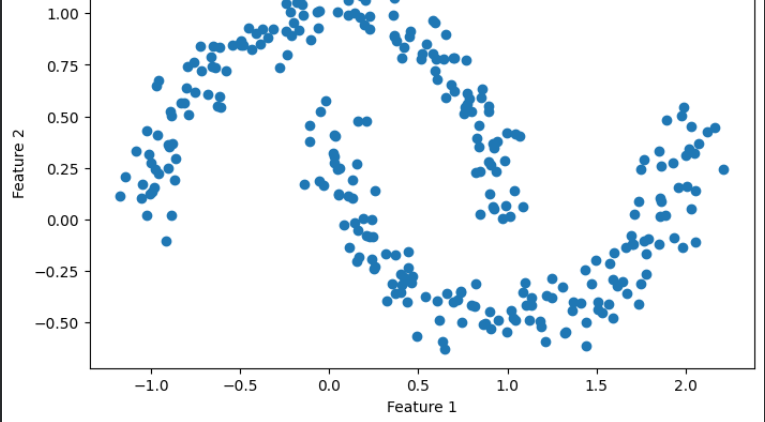
\includegraphics[width=0.75\linewidth]{dbscan_dataset.png}
    \caption{Original Moon Dataset (Before Clustering)}
    \label{fig:dbscan_dataset}
\end{figure}

\begin{figure}[H]
    \centering
    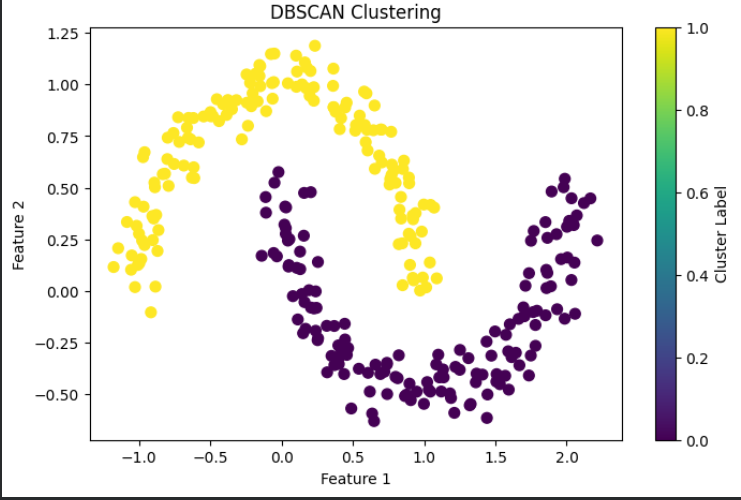
\includegraphics[width=0.75\linewidth]{dbscan_output.png}
    \caption{DBSCAN Clustering Output}
    \label{fig:dbscan_output}
\end{figure}

\paragraph{Expected Result}
The DBSCAN algorithm successfully identifies non-spherical clusters based on data density and detects noise points, without requiring the number of clusters beforehand.

\subsubsection{Discussion \& Observations}

The DBSCAN algorithm successfully identified clusters based on the density of data points in the Synthetic Moon Dataset. Unlike K-Means, DBSCAN can detect non-spherical clusters and does not require the number of clusters to be specified in advance.

The \texttt{eps} parameter controls the neighborhood radius, while \texttt{min\_samples} determines the minimum number of points required to form a dense region. Changing these parameters can affect the number of clusters and noise points.

The algorithm identifies core points, border points, and noise points based on local density. The noise points are assigned the label \texttt{-1}.

The Silhouette Score was used to evaluate the separation between detected clusters, excluding noise points from the calculation.

The experiment demonstrates that DBSCAN is useful for identifying irregularly shaped clusters and detecting outliers in a dataset.

\subsubsection{Conclusion \& Limitations}

In this experiment, DBSCAN clustering was successfully implemented using the Synthetic Moon Dataset. The algorithm identified clusters based on data density and detected noise points without requiring the number of clusters beforehand.

However, DBSCAN has some limitations. Its performance is sensitive to the selection of \texttt{eps} and \texttt{min\_samples}. It may also struggle with datasets containing clusters with different densities. Additionally, choosing a suitable epsilon value becomes difficult in high-dimensional datasets because distance measurements become less informative.

Therefore, DBSCAN is particularly useful for datasets containing irregularly shaped clusters and noise, but proper parameter selection is important for obtaining meaningful results.

% ------------------------------------------------------------
% EXPERIMENT 6
% ------------------------------------------------------------
\subsection{Experiment 6: HDBSCAN Clustering}

\subsubsection{Objective}
The objective of this experiment is to implement the HDBSCAN (Hierarchical Density-Based Spatial Clustering of Applications with Noise) algorithm to identify clusters with different density levels. Specifically, the experiment aims to:
\begin{itemize}
    \item Understand hierarchical density-based clustering.
    \item Learn how HDBSCAN improves upon DBSCAN.
    \item Identify clusters with different densities.
    \item Detect noise and outliers.
    \item Visualize the clustering results.
    \item Evaluate clustering performance using Silhouette Score.
\end{itemize}

\subsubsection{Suggested Dataset}
A \textbf{Synthetic Variable-Density Dataset} generated using \texttt{make\_blobs()} from Scikit-learn with different cluster standard deviations is used. Its configuration is:

\begin{table}[H]
\centering
\caption{Synthetic Dataset Configuration}
\begin{tabular}{ll}
\toprule
\textbf{Property} & \textbf{Value} \\
\midrule
Number of samples             & 300 \\
Number of clusters (centers)  & 3 \\
Number of features            & 2 \\
Cluster standard deviations   & 0.5, 1.0, 1.5 \\
Random state                  & 42 \\
\bottomrule
\end{tabular}
\end{table}

This dataset is suitable because it contains clusters with different density levels, allowing us to demonstrate the advantage of HDBSCAN.

\subsubsection{Required Libraries}
\begin{itemize}
    \item \textbf{NumPy} -- for numerical operations.
    \item \textbf{Matplotlib} -- for data visualization.
    \item \textbf{Scikit-learn} -- for dataset generation and evaluation.
    \item \textbf{HDBSCAN} -- for implementing hierarchical density-based clustering.
\end{itemize}

Install HDBSCAN in Google Colab:
\begin{lstlisting}[language=Python, caption={Install hdbscan}]
!pip install hdbscan
\end{lstlisting}

\begin{lstlisting}[language=Python, caption={Required Imports}]
import numpy as np
import matplotlib.pyplot as plt

import hdbscan

from sklearn.datasets import make_blobs
from sklearn.metrics import silhouette_score
\end{lstlisting}

\subsubsection{Brief Theory}
HDBSCAN stands for Hierarchical Density-Based Spatial Clustering of Applications with Noise. It is an unsupervised machine learning algorithm that identifies clusters based on density and builds a hierarchy of possible clusters.

HDBSCAN is an extension of DBSCAN. It can handle clusters with different densities more effectively by considering multiple density levels instead of relying on a single fixed epsilon value.

\paragraph{Important Parameters}
\begin{enumerate}
    \item \textbf{\texttt{min\_cluster\_size}:} Defines the minimum number of data points required to form a cluster. A smaller value may produce more clusters, while a larger value may produce fewer clusters.
    \item \textbf{\texttt{min\_samples}:} Controls how conservatively the algorithm identifies dense regions. A larger value generally makes the algorithm stricter and may classify more points as noise.
    \item \textbf{\texttt{metric}:} Defines the distance measurement used by the algorithm. Euclidean distance is commonly used for numerical datasets.
\end{enumerate}

\paragraph{Main Steps}
\begin{enumerate}
    \item Calculate distances between data points.
    \item Calculate the core distance for each point.
    \item Construct the mutual reachability distance.
    \item Build a minimum spanning tree.
    \item Create a hierarchy of clusters.
    \item Extract stable clusters from the hierarchy.
    \item Identify noise points.
\end{enumerate}

\paragraph{Core Distance}
Core distance represents the distance from a point to its specified nearest neighbor.

\paragraph{Mutual Reachability Distance}
HDBSCAN uses mutual reachability distance to construct a density-based hierarchy:
\[
d_{mr}(a, b) = \max(core_k(a), core_k(b), d(a, b))
\]
where $d_{mr}$ is the mutual reachability distance, $core_k(a)$ and $core_k(b)$ are the core distances of points $a$ and $b$, and $d(a, b)$ is the distance between the two points.

\paragraph{Difference Between DBSCAN and HDBSCAN}
\begin{table}[H]
\centering
\caption{DBSCAN vs.\ HDBSCAN}
\begin{tabular}{ll}
\toprule
\textbf{DBSCAN} & \textbf{HDBSCAN} \\
\midrule
Uses a fixed epsilon value         & Does not require a fixed epsilon \\
Works with a single density threshold & Considers multiple density levels \\
Sensitive to varying densities      & Handles varying densities more effectively \\
Identifies noise points             & Identifies noise points \\
Simpler algorithm                   & More complex hierarchical algorithm \\
\bottomrule
\end{tabular}
\end{table}

\paragraph{Evaluation Metric}
\textbf{Silhouette Score:} Measures how well-separated the detected clusters are.
\begin{itemize}
    \item Close to $1$: Well-separated clusters.
    \item Close to $0$: Overlapping clusters.
    \item Negative: Possible incorrect clustering.
\end{itemize}
Noise points are excluded from the Silhouette Score calculation in this experiment.

\subsubsection{Procedure}
\begin{enumerate}
    \item Import the required Python libraries.
    \item Install the HDBSCAN package.
    \item Generate a synthetic dataset with different cluster densities.
    \item Visualize the original dataset.
    \item Set the HDBSCAN parameters.
    \item Create the HDBSCAN model.
    \item Fit the model to the dataset.
    \item Assign cluster labels to each data point.
    \item Identify noise points using the label \texttt{-1}.
    \item Visualize the resulting clusters.
    \item Calculate the number of clusters and noise points.
    \item Calculate the Silhouette Score for valid clusters.
    \item Analyze the clustering results.
\end{enumerate}

\subsubsection{Reference Implementation}
\begin{lstlisting}[language=Python, caption={HDBSCAN Clustering Implementation}]
# ==========================================
# Experiment 6: HDBSCAN Clustering
# ==========================================

# 1. Import required libraries
import numpy as np
import matplotlib.pyplot as plt

import hdbscan

from sklearn.datasets import make_blobs
from sklearn.metrics import silhouette_score

# 2. Generate variable-density dataset
X, y = make_blobs(
    n_samples=300,
    centers=3,
    cluster_std=[0.5, 1.0, 1.5],
    random_state=42
)

# 3. Visualize original dataset
plt.figure(figsize=(8, 5))
plt.scatter(X[:, 0], X[:, 1])
plt.title("Original Variable-Density Dataset")
plt.xlabel("Feature 1")
plt.ylabel("Feature 2")
plt.show()

# ==========================================
# 4. Apply HDBSCAN
# ==========================================
clusterer = hdbscan.HDBSCAN(
    min_cluster_size=10,
    min_samples=5,
    metric='euclidean'
)
labels = clusterer.fit_predict(X)

# ==========================================
# 5. Visualize Clusters
# ==========================================
plt.figure(figsize=(8, 5))
plt.scatter(X[:, 0], X[:, 1], c=labels, cmap='viridis', s=50)
plt.title("HDBSCAN Clustering")
plt.xlabel("Feature 1")
plt.ylabel("Feature 2")
plt.colorbar(label="Cluster Label")
plt.show()

# ==========================================
# 6. Evaluation
# ==========================================
# Exclude noise points
mask = labels != -1

# Count clusters excluding noise
n_clusters = len(set(labels)) - (1 if -1 in labels else 0)

# Count noise points
n_noise = np.sum(labels == -1)

print("Evaluation Results")
print("-------------------------")
print("Number of Clusters:", n_clusters)
print("Number of Noise Points:", n_noise)

# Calculate Silhouette Score
if n_clusters >= 2 and np.sum(mask) > n_clusters:
    score = silhouette_score(X[mask], labels[mask])
    print("Silhouette Score:", score)
else:
    print("Silhouette Score: Not applicable")

# ==========================================
# 7. Display Cluster Information
# ==========================================
for i in sorted(set(labels)):
    if i == -1:
        print(f"Noise Points: {np.sum(labels == i)}")
    else:
        print(f"Cluster {i}: {np.sum(labels == i)} data points")

# ==========================================
# 8. Display Membership Probabilities
# ==========================================
print("\nMembership Probabilities (First 10 Points):")
print(clusterer.probabilities_[:10])
\end{lstlisting}

\subsubsection{Evaluation / Expected Output}

\paragraph{Output}
After running the program, two plots are produced:
\begin{itemize}
    \item A scatter plot of the original variable-density dataset showing three clusters with different density levels.
    \item A scatter plot of the HDBSCAN clustering result showing different colors for detected clusters, data points grouped by density, and noise points labeled \texttt{-1}.
\end{itemize}
The console also prints the number of clusters, noise points, Silhouette Score, and membership probabilities of the first ten data points.

\begin{table}[H]
\centering
\caption{Hyperparameters \& Results for HDBSCAN}
\begin{tabular}{ll}
\toprule
\textbf{Parameter / Metric} & \textbf{Value} \\
\midrule
Minimum Cluster Size         & 10 \\
Minimum Samples              & 5 \\
Distance Metric              & Euclidean \\
Random State                 & 42 \\
Number of Clusters           & \textit{(fill in)} \\
Number of Noise Points       & \textit{(fill in)} \\
Silhouette Score             & \textit{(fill in)} \\
\bottomrule
\end{tabular}
\end{table}

\begin{figure}[H]
    \centering
    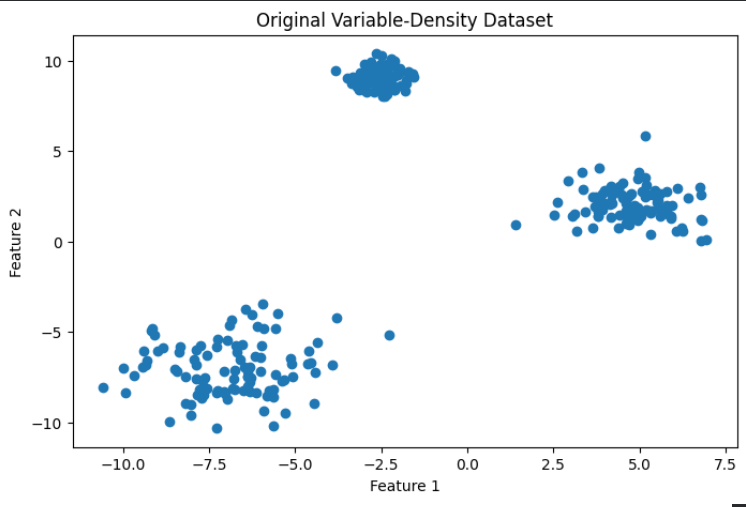
\includegraphics[width=0.75\linewidth]{hdbscan_dataset.png}
    \caption{Original Variable-Density Dataset (Before Clustering)}
    \label{fig:hdbscan_dataset}
\end{figure}

\begin{figure}[H]
    \centering
    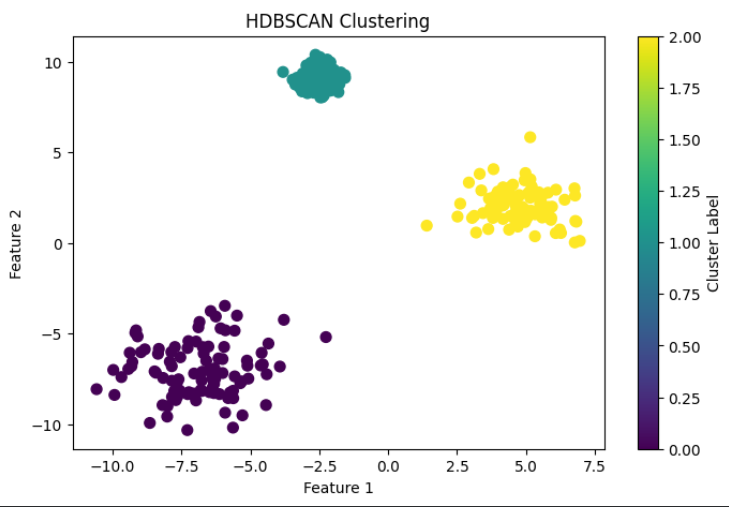
\includegraphics[width=0.75\linewidth]{hdbscan_output.png}
    \caption{HDBSCAN Clustering Output}
    \label{fig:hdbscan_output}
\end{figure}

\paragraph{Expected Result}
The HDBSCAN algorithm successfully identifies clusters with different density levels using a hierarchical density-based approach and detects noise points without requiring a fixed epsilon value.

\subsubsection{Discussion \& Observations}

The HDBSCAN algorithm successfully identified clusters based on the density structure of the dataset. Unlike DBSCAN, HDBSCAN considers multiple density levels and extracts stable clusters from a hierarchical structure.

The \texttt{min\_cluster\_size} parameter controls the minimum size required for a cluster, while \texttt{min\_samples} controls the density requirement. These parameters influence the number of detected clusters and noise points.

The algorithm also provides membership probabilities that indicate how strongly each data point belongs to its assigned cluster. Points with higher probabilities have stronger membership, while points near cluster boundaries may have lower probabilities.

The Silhouette Score was used to evaluate the separation of detected clusters, excluding noise points from the calculation.

The experiment demonstrates that HDBSCAN can handle datasets with varying densities and identify noise without requiring a fixed epsilon value.

\subsubsection{Conclusion \& Limitations}

In this experiment, HDBSCAN clustering was successfully implemented using a synthetic dataset containing clusters with different density levels. The algorithm identified clusters using a hierarchical density-based approach and detected noise points.

The experiment demonstrated that HDBSCAN provides more flexibility than DBSCAN when dealing with clusters having different densities. It also provides membership probabilities to represent the strength of cluster assignments.

However, HDBSCAN has some limitations. It is computationally more complex than DBSCAN and requires careful selection of parameters such as \texttt{min\_cluster\_size} and \texttt{min\_samples}. It may also produce unexpected results when the dataset has very high dimensions or weak density differences.

Therefore, HDBSCAN is useful for datasets containing clusters with varying densities, irregular shapes, and noise, although appropriate parameter selection is necessary for meaningful results.



% ============================================================
% SEMI-SUPERVISED LEARNING
% ============================================================
\section{Semi-Supervised Learning}

% ------------------------------------------------------------
% EXPERIMENT 7
% ------------------------------------------------------------
\subsection{Experiment 7: Self-Training for Semi-Supervised Learning}

\subsubsection{Objective}
The objective of this experiment is to implement the Self-Training technique for Semi-Supervised Learning to train a machine learning model using a small amount of labeled data and a large amount of unlabeled data. Specifically, the experiment aims to:
\begin{itemize}
    \item Understand the concept of semi-supervised learning.
    \item Learn how self-training works.
    \item Train a model using labeled data.
    \item Generate pseudo-labels for unlabeled data.
    \item Improve the training dataset using high-confidence predictions.
    \item Evaluate the model's performance using Accuracy and Classification Report.
\end{itemize}

\subsubsection{Suggested Dataset}
The \textbf{Breast Cancer Wisconsin Dataset} from Scikit-learn is used, available through the \texttt{load\_breast\_cancer()} function. Its configuration is:

\begin{table}[H]
\centering
\caption{Dataset Configuration}
\begin{tabular}{ll}
\toprule
\textbf{Property} & \textbf{Value} \\
\midrule
Number of samples  & 569 \\
Number of features & 30 \\
Number of classes  & 2 \\
Classes            & Malignant, Benign \\
\bottomrule
\end{tabular}
\end{table}

For the semi-supervised experiment:
\begin{itemize}
    \item 20\% of the training data is used as \textbf{labeled} data.
    \item 80\% of the training data is treated as \textbf{unlabeled} data.
    \item The test dataset remains fully labeled for evaluation.
\end{itemize}

This dataset is suitable because it allows us to simulate a situation where only a small portion of the available data has labels.

\subsubsection{Required Libraries}
\begin{itemize}
    \item \textbf{NumPy} -- for numerical operations.
    \item \textbf{Pandas} -- for handling dataset information.
    \item \textbf{Matplotlib} -- for visualization.
    \item \textbf{Scikit-learn} -- for data preprocessing, model training, self-training, and evaluation.
\end{itemize}

\begin{lstlisting}[language=Python, caption={Required Imports}]
import numpy as np
import pandas as pd
import matplotlib.pyplot as plt

from sklearn.datasets import load_breast_cancer
from sklearn.model_selection import train_test_split
from sklearn.preprocessing import StandardScaler
from sklearn.semi_supervised import SelfTrainingClassifier
from sklearn.svm import SVC
from sklearn.metrics import accuracy_score, classification_report
\end{lstlisting}

\subsubsection{Brief Theory}
Semi-Supervised Learning is a machine learning approach that uses both labeled and unlabeled data for training. It is useful when collecting labeled data is expensive or time-consuming, but a large amount of unlabeled data is available.

For example:
\begin{itemize}
    \item \textbf{Labeled data:} Medical images with known diagnoses.
    \item \textbf{Unlabeled data:} Medical images without diagnoses.
\end{itemize}

\paragraph{Self-Training}
Self-Training is a semi-supervised learning technique where a model uses its own predictions to generate labels for unlabeled data. The basic idea is to train a model using a small labeled dataset and then use that model to predict labels for unlabeled data.

\paragraph{Main Steps}
\begin{enumerate}
    \item Start with a small labeled dataset.
    \item Train a machine learning model using labeled data.
    \item Predict labels for the unlabeled data.
    \item Select predictions with high confidence.
    \item Add the selected pseudo-labeled data to the training dataset.
    \item Retrain the model using the expanded dataset.
    \item Repeat the process until the stopping condition is reached.
\end{enumerate}

\paragraph{Pseudo-Labeling}
A pseudo-label is a predicted label generated by a trained model for an unlabeled data point. For example, if the model predicts Class A with 95\% confidence and Class B with 5\% confidence, the model may assign Class A as the pseudo-label because it has high confidence.

\paragraph{Confidence Threshold}
The confidence threshold determines which predictions are accepted as pseudo-labels. For example, with a threshold of 0.8, only predictions with confidence greater than or equal to 0.8 are selected. A higher threshold makes the selection more conservative, while a lower threshold allows more unlabeled samples to be included.

\paragraph{Self-Training in Scikit-Learn}
Scikit-learn provides the \texttt{SelfTrainingClassifier} class for implementing self-training. Important parameters:
\begin{itemize}
    \item \texttt{estimator}: The base machine learning model.
    \item \texttt{threshold}: Minimum confidence required to accept a pseudo-label.
    \item \texttt{max\_iter}: Maximum number of self-training iterations.
    \item \texttt{verbose}: Controls the display of training information.
\end{itemize}
In this experiment, Support Vector Machine (SVM) is used as the base classifier.

\paragraph{Evaluation Metrics}
\begin{enumerate}
    \item \textbf{Accuracy:} Measures the percentage of correctly classified test samples:
    \[
    \text{Accuracy} = \frac{\text{Correct Predictions}}{\text{Total Predictions}}
    \]
    \item \textbf{Precision:} Measures how many predicted positive samples are actually positive.
    \item \textbf{Recall:} Measures how many actual positive samples are correctly identified.
    \item \textbf{F1-Score:} Represents the harmonic mean of precision and recall.
\end{enumerate}
The test data remains fully labeled and is not used during self-training.

\subsubsection{Procedure}
\begin{enumerate}
    \item Import the required Python libraries.
    \item Load the Breast Cancer Wisconsin dataset.
    \item Separate the features and target labels.
    \item Divide the dataset into training and testing sets.
    \item Apply feature scaling using \texttt{StandardScaler}.
    \item Select 20\% of the training data as labeled data.
    \item Treat the remaining 80\% of the training data as unlabeled.
    \item Replace the unlabeled labels with \texttt{-1}.
    \item Create an SVM classifier with probability estimation enabled.
    \item Apply the \texttt{SelfTrainingClassifier} with a confidence threshold of 0.8.
    \item Train the model using labeled and unlabeled data.
    \item Allow the model to generate pseudo-labels for high-confidence predictions.
    \item Evaluate the trained model using the test dataset.
    \item Display Accuracy, Precision, Recall, and F1-Score.
    \item Analyze the number of pseudo-labeled samples and the model performance.
\end{enumerate}

\subsubsection{Reference Implementation}
\begin{lstlisting}[language=Python, caption={Self-Training Implementation}]
# ==========================================
# Experiment 7: Self-Training
# Semi-Supervised Learning
# ==========================================

# 1. Import required libraries
import numpy as np
import pandas as pd
import matplotlib.pyplot as plt

from sklearn.datasets import load_breast_cancer
from sklearn.model_selection import train_test_split
from sklearn.preprocessing import StandardScaler

from sklearn.semi_supervised import SelfTrainingClassifier
from sklearn.svm import SVC

from sklearn.metrics import (
    accuracy_score,
    classification_report
)

# ==========================================
# 2. Load Dataset
# ==========================================
data = load_breast_cancer()

X = data.data
y = data.target

print("Dataset Shape:", X.shape)
print("Class Names:", data.target_names)

# ==========================================
# 3. Split Dataset
# ==========================================
X_train, X_test, y_train, y_test = train_test_split(
    X,
    y,
    test_size=0.2,
    random_state=42,
    stratify=y
)

# ==========================================
# 4. Feature Scaling
# ==========================================
scaler = StandardScaler()

X_train = scaler.fit_transform(X_train)
X_test = scaler.transform(X_test)

# ==========================================
# 5. Select Labeled and Unlabeled Data
# ==========================================
# Select 20% labeled data
# Remaining 80% will be unlabeled

indices = np.arange(len(X_train))

labeled_indices, unlabeled_indices = train_test_split(
    indices,
    test_size=0.8,
    random_state=42,
    stratify=y_train
)

# Create semi-supervised labels
y_semi = np.full(len(y_train), -1)

# Assign actual labels to labeled samples
y_semi[labeled_indices] = y_train[labeled_indices]

print("\nDataset Information")
print("-------------------------")
print("Total Training Samples:", len(X_train))
print("Labeled Samples:", len(labeled_indices))
print("Unlabeled Samples:", len(unlabeled_indices))

# ==========================================
# 6. Create Base Classifier
# ==========================================
base_model = SVC(
    probability=True,
    random_state=42
)

# ==========================================
# 7. Apply Self-Training
# ==========================================
self_training = SelfTrainingClassifier(
    estimator=base_model,
    threshold=0.8,
    max_iter=10,
    verbose=True
)

# Train using labeled and unlabeled data
self_training.fit(X_train, y_semi)

# ==========================================
# 8. Generate Predictions
# ==========================================
y_pred = self_training.predict(X_test)

# ==========================================
# 9. Evaluation
# ==========================================
accuracy = accuracy_score(y_test, y_pred)

print("\nEvaluation Results")
print("-------------------------")
print("Accuracy:", accuracy)

print("\nClassification Report:")
print(
    classification_report(
        y_test,
        y_pred,
        target_names=data.target_names
    )
)

# ==========================================
# 10. Pseudo-Label Information
# ==========================================
# Count samples that received pseudo-labels
pseudo_labeled = np.sum(
    self_training.transduction_[unlabeled_indices] != -1
)

print("\nSelf-Training Information")
print("-------------------------")
print("Initial Labeled Samples:", len(labeled_indices))
print("Initial Unlabeled Samples:", len(unlabeled_indices))
print("Pseudo-Labeled Samples:", pseudo_labeled)
print("Final Labeled Samples:",
      np.sum(self_training.transduction_ != -1))
print("Number of Iterations:", self_training.n_iter_)
\end{lstlisting}

\subsubsection{Evaluation / Expected Output}

\paragraph{Output}
After running the program, the console prints the dataset information, evaluation metrics (Accuracy and Classification Report), and self-training information (number of pseudo-labeled samples and iterations). The test data is never used for generating pseudo-labels.

\begin{table}[H]
\centering
\caption{Hyperparameters \& Setup for Self-Training}
\begin{tabular}{ll}
\toprule
\textbf{Parameter / Setting} & \textbf{Value} \\
\midrule
Base Estimator                 & SVM (RBF Kernel) with \texttt{probability=True} \\
Confidence Threshold           & 0.8 \\
Maximum Iterations             & 10 \\
Test Size                      & 0.2 \\
Labeled Fraction (of train)    & 20\% \\
Unlabeled Fraction (of train)  & 80\% \\
Random State                   & 42 \\
\bottomrule
\end{tabular}
\end{table}

\begin{table}[H]
\centering
\caption{Results for Self-Training}
\begin{tabular}{ll}
\toprule
\textbf{Metric} & \textbf{Value} \\
\midrule
Total Training Samples     & 455 \\
Initial Labeled Samples    & 91 \\
Initial Unlabeled Samples  & 364 \\
Pseudo-Labeled Samples     & \textit{(fill in)} \\
Final Labeled Samples      & \textit{(fill in)} \\
Number of Iterations       & \textit{(fill in)} \\
Accuracy                   & \textit{(fill in)} \\
\bottomrule
\end{tabular}
\end{table}

\begin{figure}[H]
    \centering
    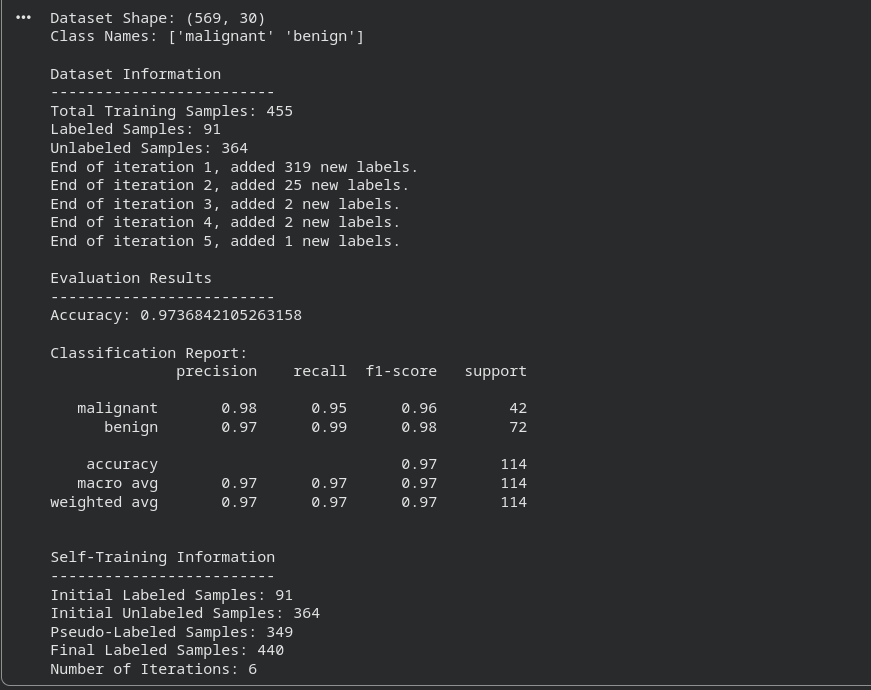
\includegraphics[width=0.85\linewidth]{selftrain_output.png}
    \caption{Self-Training Output: Evaluation Metrics and Pseudo-Label Information}
    \label{fig:selftrain_output}
\end{figure}

\paragraph{Expected Result}
The Self-Training algorithm uses the initially labeled samples to train an SVM model. It then predicts labels for the unlabeled samples and adds high-confidence predictions to the training dataset. The model is expected to classify the test samples using the information learned from both original labeled data and newly generated pseudo-labels.

\subsubsection{Discussion \& Observations}

The Self-Training algorithm was successfully implemented using the Breast Cancer Wisconsin dataset. Initially, only 20\% of the training samples were provided with actual labels, while the remaining 80\% were treated as unlabeled data.

The SVM classifier was used as the base model to generate predictions for the unlabeled samples. The confidence threshold of 0.8 ensured that only high-confidence predictions were selected as pseudo-labels.

The selected pseudo-labeled samples were added to the training process, allowing the model to learn from additional data without requiring manually assigned labels.

The Accuracy and Classification Report were used to evaluate the model's performance on the test dataset. The number of pseudo-labeled samples also helped demonstrate how much unlabeled data was successfully utilized.

However, pseudo-labeling may introduce incorrect labels if the model makes confident but wrong predictions. Therefore, selecting an appropriate confidence threshold is important for maintaining model reliability.

\subsubsection{Conclusion \& Limitations}

In this experiment, the Self-Training technique was successfully implemented for Semi-Supervised Learning using an SVM classifier.

The experiment demonstrated how a model can learn from a small amount of labeled data and use its own high-confidence predictions to generate pseudo-labels for unlabeled data.

The technique helps reduce dependence on manually labeled datasets and can improve learning when sufficient useful unlabeled data is available.

However, Self-Training has some limitations. Incorrect pseudo-labels may negatively affect the model's performance. The algorithm is also sensitive to the confidence threshold and the quality of the initial labeled dataset. If the initial model performs poorly, it may generate incorrect pseudo-labels that accumulate during training.

Therefore, Self-Training is useful when labeled data is limited but unlabeled data is available, provided that the initial model produces reasonably reliable predictions.


% ============================================================
% ENSEMBLE LEARNING
% ============================================================
\section{Ensemble Learning}

% ------------------------------------------------------------
% EXPERIMENT 8
% ------------------------------------------------------------
\subsection{Experiment 8: Random Forest Regression (RFR)}

\subsubsection{Objective}
To implement Random Forest Regression and predict continuous values using multiple decision trees. The performance of the model will be evaluated using regression metrics.

\subsubsection{Suggested Dataset}
The \textbf{California Housing Dataset} from Scikit-learn is used. Its configuration is:

\begin{table}[H]
\centering
\caption{Dataset Configuration}
\begin{tabular}{ll}
\toprule
\textbf{Property} & \textbf{Value} \\
\midrule
Source             & \texttt{fetch\_california\_housing()} \\
Number of samples  & 20{,}640 \\
Number of features & 8 \\
Target             & Median house value \\
\bottomrule
\end{tabular}
\end{table}

The dataset contains information about houses in different areas of California. Features include income, house age, number of rooms, and population.

\subsubsection{Required Libraries}
\begin{itemize}
    \item \textbf{NumPy} -- for numerical operations.
    \item \textbf{Pandas} -- for handling dataset information.
    \item \textbf{Matplotlib} -- for visualization.
    \item \textbf{Scikit-learn} -- for dataset loading, model training, and evaluation.
\end{itemize}

\begin{lstlisting}[language=Python, caption={Required Imports}]
import numpy as np
import pandas as pd
import matplotlib.pyplot as plt

from sklearn.datasets import fetch_california_housing
from sklearn.model_selection import train_test_split
from sklearn.ensemble import RandomForestRegressor
from sklearn.metrics import (
    mean_absolute_error,
    mean_squared_error,
    r2_score
)
\end{lstlisting}

\subsubsection{Brief Theory}
Random Forest Regression is an \textbf{ensemble learning algorithm} that combines multiple Decision Tree Regressors to make predictions. Each tree is trained using a random sample of the training data and a random subset of features. The final prediction is calculated by taking the average of predictions from all trees.

\paragraph{Main Advantages}
\begin{itemize}
    \item Reduces overfitting compared to a single decision tree.
    \item Handles complex and non-linear relationships.
    \item Usually provides stable predictions.
\end{itemize}

\paragraph{Important Parameters}
\begin{itemize}
    \item \texttt{n\_estimators}: Number of decision trees.
    \item \texttt{max\_depth}: Maximum depth of each tree.
    \item \texttt{random\_state}: Controls randomness for reproducible results.
\end{itemize}

\paragraph{Evaluation Metrics}
\begin{table}[H]
\centering
\caption{Regression Evaluation Metrics}
\begin{tabular}{ll}
\toprule
\textbf{Metric} & \textbf{Meaning} \\
\midrule
MAE      & Average absolute prediction error \\
MSE      & Average squared prediction error \\
RMSE     & Square root of MSE \\
R$^2$ Score & Measures how well the model explains variation in the target \\
\bottomrule
\end{tabular}
\end{table}

A lower MAE, MSE, and RMSE generally indicate better predictions. An R$^2$ score closer to 1 indicates that the model explains more variation in the target values.

\subsubsection{Procedure}
\begin{enumerate}
    \item Import the required libraries.
    \item Load the California Housing dataset.
    \item Separate the features and target variable.
    \item Split the dataset into training and testing sets.
    \item Create a Random Forest Regressor model.
    \item Train the model using the training data.
    \item Predict house values using the test data.
    \item Evaluate the model using MAE, MSE, RMSE, and R$^2$ score.
    \item Visualize actual values against predicted values.
\end{enumerate}

\subsubsection{Reference Implementation}
\begin{lstlisting}[language=Python, caption={Random Forest Regression Implementation}]
# Step 1: Import required libraries
import numpy as np
import pandas as pd
import matplotlib.pyplot as plt

from sklearn.datasets import fetch_california_housing
from sklearn.model_selection import train_test_split
from sklearn.ensemble import RandomForestRegressor
from sklearn.metrics import (
    mean_absolute_error,
    mean_squared_error,
    r2_score
)

# Step 2: Load the dataset
data = fetch_california_housing()
X = data.data
y = data.target

print("Dataset shape:", X.shape)
print("Feature names:", data.feature_names)

# Step 3: Split the dataset
X_train, X_test, y_train, y_test = train_test_split(
    X, y,
    test_size=0.2,
    random_state=42
)

# Step 4: Create the Random Forest Regression model
model = RandomForestRegressor(
    n_estimators=100,
    random_state=42,
    n_jobs=-1
)

# Step 5: Train the model
model.fit(X_train, y_train)

# Step 6: Make predictions
y_pred = model.predict(X_test)

# Step 7: Evaluate the model
mae = mean_absolute_error(y_test, y_pred)
mse = mean_squared_error(y_test, y_pred)
rmse = np.sqrt(mse)
r2 = r2_score(y_test, y_pred)

print("\nModel Evaluation:")
print("MAE:", mae)
print("MSE:", mse)
print("RMSE:", rmse)
print("R2 Score:", r2)

# Step 8: Compare actual and predicted values
comparison = pd.DataFrame({
    "Actual Value": y_test[:10],
    "Predicted Value": y_pred[:10]
})
print("\nActual vs Predicted Values:")
print(comparison)

# Step 9: Visualize actual vs predicted values
plt.figure(figsize=(8, 6))
plt.scatter(y_test, y_pred, alpha=0.5)
plt.xlabel("Actual House Values")
plt.ylabel("Predicted House Values")
plt.title("Random Forest Regression: Actual vs Predicted")

# Reference line
min_value = min(y_test.min(), y_pred.min())
max_value = max(y_test.max(), y_pred.max())
plt.plot([min_value, max_value], [min_value, max_value], "r--")
plt.show()
\end{lstlisting}

\subsubsection{Evaluation / Expected Output}

\paragraph{Output}
After running the program, the console prints the dataset shape and feature names, the regression metrics (MAE, MSE, RMSE, R$^2$), and a table comparing the first 10 actual vs.\ predicted values. A scatter plot of actual vs.\ predicted values is also produced.

\begin{table}[H]
\centering
\caption{Hyperparameters \& Setup for Random Forest Regression}
\begin{tabular}{ll}
\toprule
\textbf{Parameter / Setting} & \textbf{Value} \\
\midrule
Number of Estimators (\texttt{n\_estimators}) & 100 \\
Maximum Depth (\texttt{max\_depth})           & Default (None) \\
Random State                                   & 42 \\
Test Size                                      & 0.2 \\
Parallel Jobs (\texttt{n\_jobs})               & $-1$ (all cores) \\
\bottomrule
\end{tabular}
\end{table}

\begin{table}[H]
\centering
\caption{Regression Results}
\begin{tabular}{ll}
\toprule
\textbf{Metric} & \textbf{Value} \\
\midrule
MAE       & \textit{(fill in)} \\
MSE       & \textit{(fill in)} \\
RMSE      & \textit{(fill in)} \\
R$^2$ Score & \textit{(fill in)} \\
\bottomrule
\end{tabular}
\end{table}

\begin{figure}[H]
    \centering
    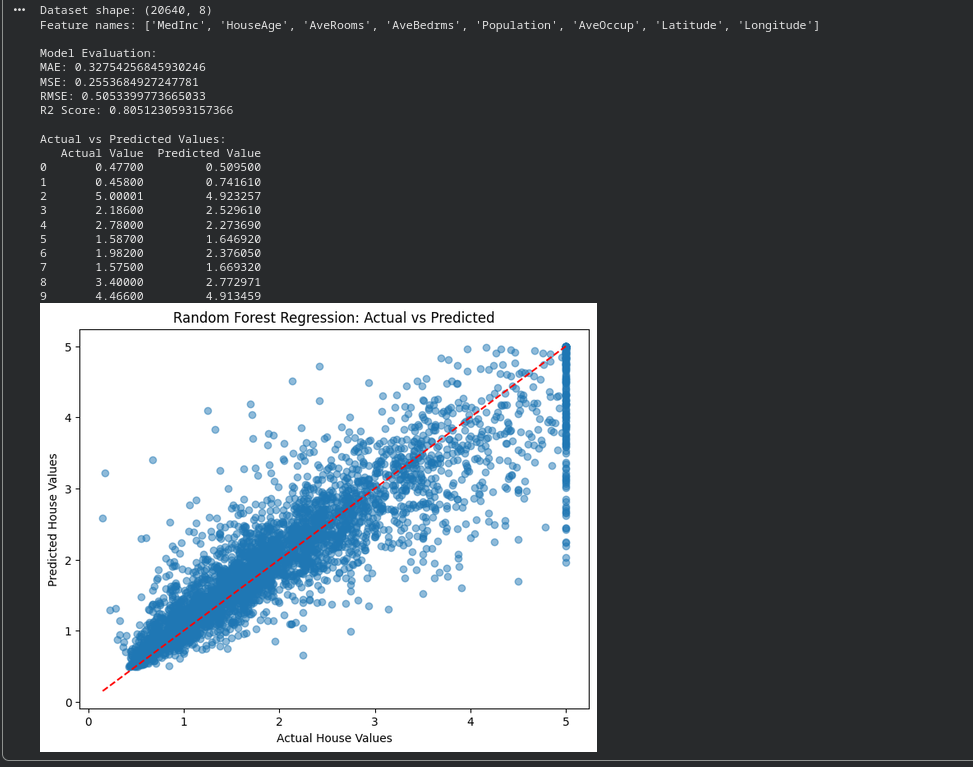
\includegraphics[width=0.75\linewidth]{rfr_output.png}
    \caption{Random Forest Regression: Actual vs.\ Predicted House Values}
    \label{fig:rfr_output}
\end{figure}

\paragraph{Expected Result}
The Random Forest Regression model successfully predicts median house values using the California Housing dataset. The evaluation metrics indicate the prediction accuracy, and the scatter plot shows a positive relationship between actual and predicted values, with points clustered near the red reference line.

\subsubsection{Discussion \& Observations}

Random Forest uses multiple decision trees to improve prediction stability. The model predicts continuous values instead of class labels.

The actual and predicted values should show a positive relationship in the scatter plot. Points closer to the red reference line indicate more accurate predictions.

The model may perform less accurately for house values that are difficult to predict from the available features. The R$^2$ score indicates how well the model explains the variance in the target values, while MAE, MSE, and RMSE quantify the average prediction error in different ways.

Increasing \texttt{n\_estimators} generally improves stability at the cost of longer training time, while limiting \texttt{max\_depth} can control overfitting.

\subsubsection{Conclusion \& Limitations}

Random Forest Regression was implemented using the California Housing dataset. The model was trained to predict median house values, and its performance was evaluated using MAE, MSE, RMSE, and R$^2$ score.

\textbf{Limitations:}
\begin{itemize}
    \item Training can be slower when many trees are used.
    \item The model may require parameter tuning for better performance.
    \item Predictions are limited by the quality and information available in the dataset.
\end{itemize}



% ------------------------------------------------------------
% EXPERIMENT 9
% ------------------------------------------------------------
\subsection{Experiment 9: Random Forest Classification (RFC)}

\subsubsection{Objective}
To implement Random Forest Classification and predict class labels using multiple decision trees. The model's performance will be evaluated using classification metrics.

\subsubsection{Suggested Dataset}
The \textbf{Breast Cancer Wisconsin Dataset} from Scikit-learn is used. Its configuration is:

\begin{table}[H]
\centering
\caption{Dataset Configuration}
\begin{tabular}{ll}
\toprule
\textbf{Property} & \textbf{Value} \\
\midrule
Source             & \texttt{load\_breast\_cancer()} \\
Number of samples  & 569 \\
Number of features & 30 \\
Number of classes  & 2 \\
Classes            & 0 = Malignant, 1 = Benign \\
\bottomrule
\end{tabular}
\end{table}

The dataset contains features calculated from breast cancer cell nuclei, and the target indicates whether the tumor is malignant or benign.

\subsubsection{Required Libraries}
\begin{itemize}
    \item \textbf{NumPy} -- for numerical operations.
    \item \textbf{Pandas} -- for handling dataset information and feature importance.
    \item \textbf{Matplotlib} -- for visualization.
    \item \textbf{Scikit-learn} -- for dataset loading, model training, and evaluation.
\end{itemize}

\begin{lstlisting}[language=Python, caption={Required Imports}]
import numpy as np
import pandas as pd
import matplotlib.pyplot as plt

from sklearn.datasets import load_breast_cancer
from sklearn.model_selection import train_test_split
from sklearn.ensemble import RandomForestClassifier
from sklearn.metrics import (
    accuracy_score,
    classification_report,
    confusion_matrix,
    ConfusionMatrixDisplay
)
\end{lstlisting}

\subsubsection{Brief Theory}
Random Forest Classification is an \textbf{ensemble learning algorithm} that combines multiple Decision Tree Classifiers to predict a class. Each tree is trained using a random sample of the training data and a random subset of features. The final prediction is made by \textbf{majority voting} among all trees.

\paragraph{Main Advantages}
\begin{itemize}
    \item Reduces overfitting compared to a single decision tree.
    \item Handles complex data.
    \item Provides stable classification results.
    \item Can measure feature importance.
\end{itemize}

\paragraph{Important Parameters}
\begin{itemize}
    \item \texttt{n\_estimators}: Number of decision trees.
    \item \texttt{max\_depth}: Maximum depth of each tree.
    \item \texttt{random\_state}: Controls randomness for reproducible results.
\end{itemize}

\paragraph{Evaluation Metrics}
\begin{table}[H]
\centering
\caption{Classification Evaluation Metrics}
\begin{tabular}{ll}
\toprule
\textbf{Metric} & \textbf{Meaning} \\
\midrule
Accuracy         & Percentage of correct predictions \\
Precision        & How many predicted positive cases are actually positive \\
Recall           & How many actual positive cases are correctly identified \\
F1-score         & Harmonic mean of precision and recall \\
Confusion Matrix & Shows correct and incorrect predictions for each class \\
\bottomrule
\end{tabular}
\end{table}

\subsubsection{Procedure}
\begin{enumerate}
    \item Import the required libraries.
    \item Load the Breast Cancer Wisconsin dataset.
    \item Separate the features and target variable.
    \item Split the dataset into training and testing sets.
    \item Create a Random Forest Classifier model.
    \item Train the model using the training data.
    \item Predict class labels using the test data.
    \item Evaluate the model using accuracy, precision, recall, and F1-score.
    \item Display the confusion matrix.
    \item Visualize the feature importance.
\end{enumerate}

\subsubsection{Reference Implementation}
\begin{lstlisting}[language=Python, caption={Random Forest Classification Implementation}]
# Step 1: Import required libraries
import numpy as np
import pandas as pd
import matplotlib.pyplot as plt

from sklearn.datasets import load_breast_cancer
from sklearn.model_selection import train_test_split
from sklearn.ensemble import RandomForestClassifier
from sklearn.metrics import (
    accuracy_score,
    classification_report,
    confusion_matrix,
    ConfusionMatrixDisplay
)

# Step 2: Load the dataset
data = load_breast_cancer()
X = data.data
y = data.target

print("Dataset shape:", X.shape)
print("Feature names:", data.feature_names)
print("Target classes:", data.target_names)

# Step 3: Split the dataset
X_train, X_test, y_train, y_test = train_test_split(
    X, y,
    test_size=0.2,
    random_state=42,
    stratify=y
)

# Step 4: Create the Random Forest Classifier
model = RandomForestClassifier(
    n_estimators=100,
    random_state=42,
    n_jobs=-1
)

# Step 5: Train the model
model.fit(X_train, y_train)

# Step 6: Make predictions
y_pred = model.predict(X_test)

# Step 7: Evaluate the model
accuracy = accuracy_score(y_test, y_pred)

print("\nModel Evaluation:")
print("Accuracy:", accuracy)

print("\nClassification Report:")
print(classification_report(
    y_test,
    y_pred,
    target_names=data.target_names
))

# Step 8: Display confusion matrix
cm = confusion_matrix(y_test, y_pred)

disp = ConfusionMatrixDisplay(
    confusion_matrix=cm,
    display_labels=data.target_names
)
disp.plot(cmap="Blues")
plt.title("Random Forest Classification - Confusion Matrix")
plt.show()

# Step 9: Visualize feature importance
importance = model.feature_importances_

feature_importance = pd.Series(
    importance,
    index=data.feature_names
).sort_values(ascending=False)

plt.figure(figsize=(10, 6))
feature_importance.head(10).plot(kind="bar")
plt.title("Top 10 Feature Importances")
plt.xlabel("Features")
plt.ylabel("Importance")
plt.xticks(rotation=45, ha="right")
plt.tight_layout()
plt.show()
\end{lstlisting}

\subsubsection{Evaluation / Expected Output}

\paragraph{Output}
After running the program, the console prints the dataset shape, feature names, target classes, accuracy score, and the classification report. Two plots are produced:
\begin{itemize}
    \item A confusion matrix showing correct and incorrect predictions for each class.
    \item A bar chart of the top 10 most important features.
\end{itemize}

\begin{table}[H]
\centering
\caption{Hyperparameters \& Setup for Random Forest Classification}
\begin{tabular}{ll}
\toprule
\textbf{Parameter / Setting} & \textbf{Value} \\
\midrule
Number of Estimators (\texttt{n\_estimators}) & 100 \\
Maximum Depth (\texttt{max\_depth})           & Default (None) \\
Random State                                   & 42 \\
Test Size                                      & 0.2 \\
Stratified Split                               & Yes \\
Parallel Jobs (\texttt{n\_jobs})               & $-1$ (all cores) \\
\bottomrule
\end{tabular}
\end{table}

\begin{table}[H]
\centering
\caption{Classification Results}
\begin{tabular}{ll}
\toprule
\textbf{Metric} & \textbf{Value} \\
\midrule
Accuracy         & \textit{(fill in)} \\
Precision (Malignant) & \textit{(fill in)} \\
Recall (Malignant)    & \textit{(fill in)} \\
F1-score (Malignant)  & \textit{(fill in)} \\
Precision (Benign)    & \textit{(fill in)} \\
Recall (Benign)       & \textit{(fill in)} \\
F1-score (Benign)     & \textit{(fill in)} \\
\bottomrule
\end{tabular}
\end{table}

\begin{figure}[H]
    \centering
    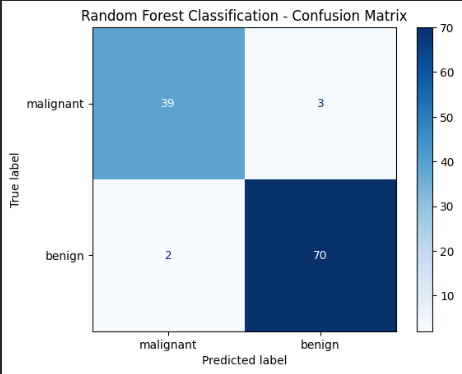
\includegraphics[width=0.7\linewidth]{rfc_confusion_matrix.png}
    \caption{Random Forest Classification: Confusion Matrix}
    \label{fig:rfc_confusion}
\end{figure}

\begin{figure}[H]
    \centering
    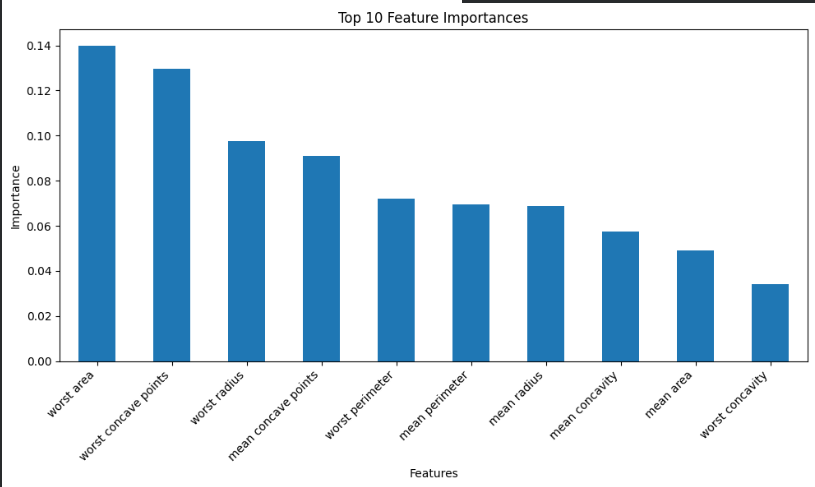
\includegraphics[width=0.85\linewidth]{rfc_feature_importance.png}
    \caption{Top 10 Feature Importances}
    \label{fig:rfc_importance}
\end{figure}

\paragraph{Expected Result}
The Random Forest Classifier successfully classifies tumors as malignant or benign using the Breast Cancer Wisconsin dataset. The accuracy is generally high, and the confusion matrix and feature importance plot provide insight into model behavior and the most influential features.

\subsubsection{Discussion \& Observations}

Random Forest combines multiple decision trees using majority voting. The model predicts discrete class labels and generally achieves high accuracy on this dataset.

The confusion matrix helps identify correct and incorrect classifications for each class, while the classification report provides precision, recall, and F1-score for a more detailed performance assessment.

Feature importance shows which features contributed more to the model's predictions. This is useful for understanding the data and identifying the most informative features, but it does not imply causation.

The model can classify complex data without requiring feature scaling, making it convenient for datasets with features on different scales.

\subsubsection{Conclusion \& Limitations}

Random Forest Classification was implemented using the Breast Cancer Wisconsin dataset. The model was trained to classify tumors as malignant or benign and evaluated using accuracy, precision, recall, F1-score, and a confusion matrix.

\textbf{Limitations:}
\begin{itemize}
    \item Training can be slower when many trees are used.
    \item The model may require parameter tuning for optimal performance.
    \item Feature importance does not prove that a feature causes a particular outcome.
\end{itemize}




% ------------------------------------------------------------
% EXPERIMENT 10
% ------------------------------------------------------------
\subsection{Experiment 10: XGBoost}

\subsubsection{Objective}
To implement XGBoost (Extreme Gradient Boosting) for classification and evaluate its performance using classification metrics.

\subsubsection{Suggested Dataset}
The \textbf{Breast Cancer Wisconsin Dataset} from Scikit-learn is used. Its configuration is:

\begin{table}[H]
\centering
\caption{Dataset Configuration}
\begin{tabular}{ll}
\toprule
\textbf{Property} & \textbf{Value} \\
\midrule
Source             & \texttt{load\_breast\_cancer()} \\
Number of samples  & 569 \\
Number of features & 30 \\
Number of classes  & 2 \\
Classes            & 0 = Malignant, 1 = Benign \\
\bottomrule
\end{tabular}
\end{table}

The dataset contains features calculated from breast cancer cell nuclei, and the target indicates whether the tumor is malignant or benign.

\subsubsection{Required Libraries}
\begin{itemize}
    \item \textbf{NumPy} -- for numerical operations.
    \item \textbf{Pandas} -- for handling dataset information and feature importance.
    \item \textbf{Matplotlib} -- for visualization.
    \item \textbf{Scikit-learn} -- for dataset loading and evaluation.
    \item \textbf{XGBoost} -- for the gradient boosting classifier.
\end{itemize}

Install XGBoost in Google Colab:
\begin{lstlisting}[language=Python, caption={Install xgboost}]
!pip install xgboost
\end{lstlisting}

\begin{lstlisting}[language=Python, caption={Required Imports}]
import numpy as np
import pandas as pd
import matplotlib.pyplot as plt

from xgboost import XGBClassifier
from sklearn.datasets import load_breast_cancer
from sklearn.model_selection import train_test_split
from sklearn.metrics import (
    accuracy_score,
    classification_report,
    confusion_matrix,
    ConfusionMatrixDisplay
)
\end{lstlisting}

\subsubsection{Brief Theory}
XGBoost is an \textbf{ensemble learning algorithm} based on Gradient Boosting. It builds decision trees \textbf{sequentially}, where each new tree tries to correct the errors made by previous trees. It uses \textbf{regularization} to reduce overfitting and improve model performance.

\paragraph{Main Advantages}
\begin{itemize}
    \item Provides high prediction accuracy.
    \item Handles complex relationships in data.
    \item Includes regularization to reduce overfitting.
    \item Supports feature importance analysis.
\end{itemize}

\paragraph{Important Parameters}
\begin{itemize}
    \item \texttt{n\_estimators}: Number of boosting rounds (trees).
    \item \texttt{max\_depth}: Maximum depth of each tree.
    \item \texttt{learning\_rate}: Controls the contribution of each new tree.
    \item \texttt{random\_state}: Controls randomness for reproducible results.
\end{itemize}

\paragraph{Evaluation Metrics}
\begin{table}[H]
\centering
\caption{Classification Evaluation Metrics}
\begin{tabular}{ll}
\toprule
\textbf{Metric} & \textbf{Meaning} \\
\midrule
Accuracy         & Percentage of correct predictions \\
Precision        & How many predicted positive cases are actually positive \\
Recall           & How many actual positive cases are correctly identified \\
F1-score         & Harmonic mean of precision and recall \\
Confusion Matrix & Shows correct and incorrect predictions for each class \\
\bottomrule
\end{tabular}
\end{table}

\subsubsection{Procedure}
\begin{enumerate}
    \item Import the required libraries.
    \item Load the Breast Cancer Wisconsin dataset.
    \item Separate the features and target variable.
    \item Split the dataset into training and testing sets.
    \item Create an XGBoost classifier.
    \item Train the model using the training data.
    \item Predict class labels using the test data.
    \item Evaluate the model using accuracy, precision, recall, and F1-score.
    \item Display the confusion matrix.
    \item Visualize feature importance.
\end{enumerate}

\subsubsection{Reference Implementation}
\begin{lstlisting}[language=Python, caption={XGBoost Classification Implementation}]
# Step 1: Import required libraries
import numpy as np
import pandas as pd
import matplotlib.pyplot as plt

from xgboost import XGBClassifier
from sklearn.datasets import load_breast_cancer
from sklearn.model_selection import train_test_split
from sklearn.metrics import (
    accuracy_score,
    classification_report,
    confusion_matrix,
    ConfusionMatrixDisplay
)

# Step 2: Load the dataset
data = load_breast_cancer()
X = data.data
y = data.target

print("Dataset shape:", X.shape)
print("Feature names:", data.feature_names)
print("Target classes:", data.target_names)

# Step 3: Split the dataset
X_train, X_test, y_train, y_test = train_test_split(
    X, y,
    test_size=0.2,
    random_state=42,
    stratify=y
)

# Step 4: Create the XGBoost classifier
model = XGBClassifier(
    n_estimators=100,
    max_depth=3,
    learning_rate=0.1,
    objective="binary:logistic",
    eval_metric="logloss",
    random_state=42
)

# Step 5: Train the model
model.fit(X_train, y_train)

# Step 6: Make predictions
y_pred = model.predict(X_test)

# Step 7: Evaluate the model
accuracy = accuracy_score(y_test, y_pred)

print("\nModel Evaluation:")
print("Accuracy:", accuracy)

print("\nClassification Report:")
print(classification_report(
    y_test,
    y_pred,
    target_names=data.target_names
))

# Step 8: Display confusion matrix
cm = confusion_matrix(y_test, y_pred)

disp = ConfusionMatrixDisplay(
    confusion_matrix=cm,
    display_labels=data.target_names
)
disp.plot(cmap="Blues")
plt.title("XGBoost - Confusion Matrix")
plt.show()

# Step 9: Visualize feature importance
importance = model.feature_importances_

feature_importance = pd.Series(
    importance,
    index=data.feature_names
).sort_values(ascending=False)

plt.figure(figsize=(10, 6))
feature_importance.head(10).plot(kind="bar")
plt.title("XGBoost - Top 10 Feature Importances")
plt.xlabel("Features")
plt.ylabel("Importance")
plt.xticks(rotation=45, ha="right")
plt.tight_layout()
plt.show()
\end{lstlisting}

\subsubsection{Evaluation / Expected Output}

\paragraph{Output}
After running the program, the console prints the dataset shape, feature names, target classes, accuracy score, and the classification report. Two plots are produced:
\begin{itemize}
    \item A confusion matrix showing correct and incorrect predictions for each class.
    \item A bar chart of the top 10 most important features.
\end{itemize}

\begin{table}[H]
\centering
\caption{Hyperparameters \& Setup for XGBoost}
\begin{tabular}{ll}
\toprule
\textbf{Parameter / Setting} & \textbf{Value} \\
\midrule
Number of Estimators (\texttt{n\_estimators}) & 100 \\
Maximum Depth (\texttt{max\_depth})           & 3 \\
Learning Rate (\texttt{learning\_rate})       & 0.1 \\
Objective                                      & \texttt{binary:logistic} \\
Evaluation Metric                              & \texttt{logloss} \\
Random State                                   & 42 \\
Test Size                                      & 0.2 \\
Stratified Split                               & Yes \\
\bottomrule
\end{tabular}
\end{table}

\begin{table}[H]
\centering
\caption{Classification Results}
\begin{tabular}{ll}
\toprule
\textbf{Metric} & \textbf{Value} \\
\midrule
Accuracy              & \textit{(fill in)} \\
Precision (Malignant) & \textit{(fill in)} \\
Recall (Malignant)    & \textit{(fill in)} \\
F1-score (Malignant)  & \textit{(fill in)} \\
Precision (Benign)    & \textit{(fill in)} \\
Recall (Benign)       & \textit{(fill in)} \\
F1-score (Benign)     & \textit{(fill in)} \\
\bottomrule
\end{tabular}
\end{table}

\begin{figure}[H]
    \centering
    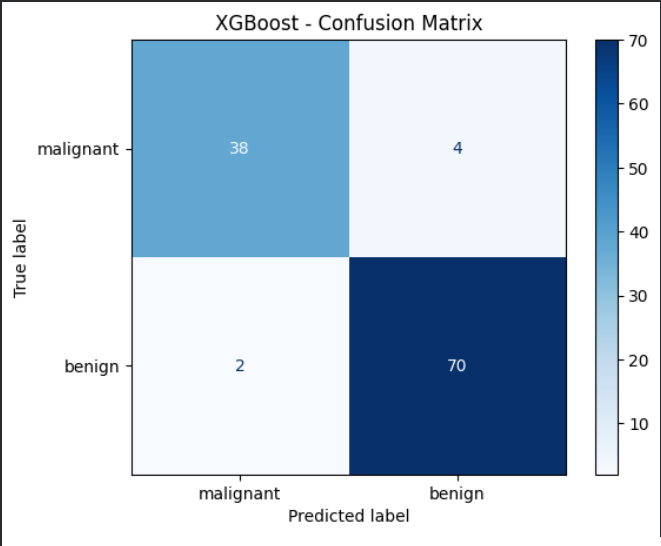
\includegraphics[width=0.7\linewidth]{xgb_confusion_matrix.png}
    \caption{XGBoost: Confusion Matrix}
    \label{fig:xgb_confusion}
\end{figure}

\begin{figure}[H]
    \centering
    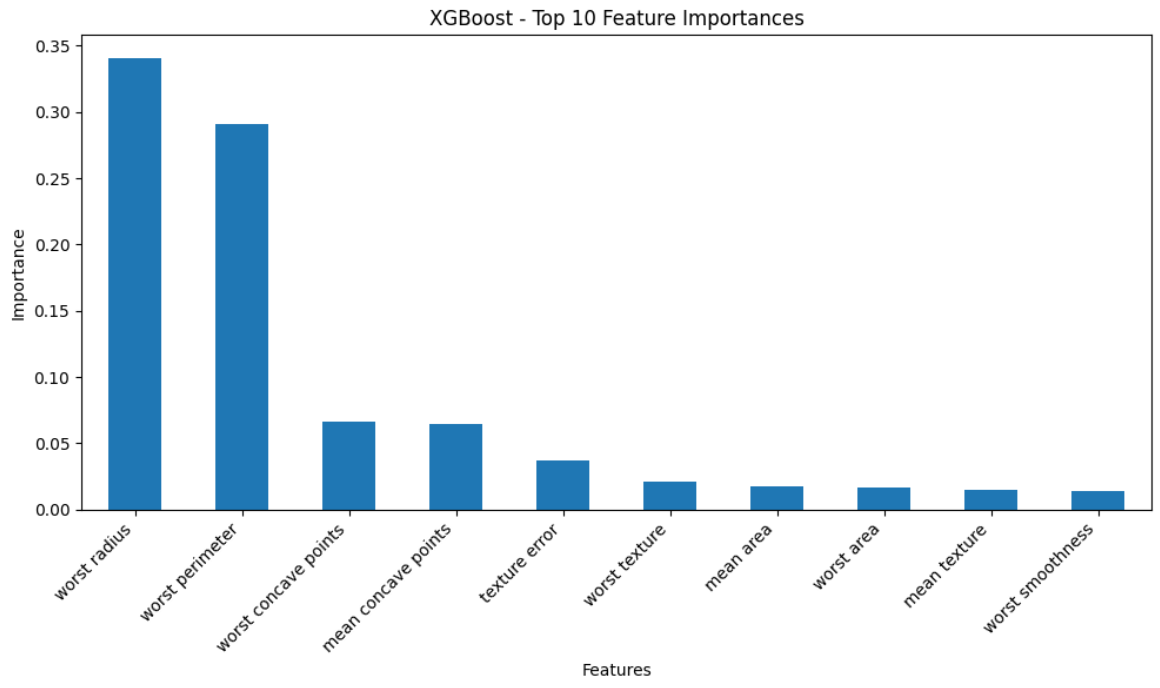
\includegraphics[width=0.85\linewidth]{xgb_feature_importance.png}
    \caption{XGBoost: Top 10 Feature Importances}
    \label{fig:xgb_importance}
\end{figure}

\paragraph{Expected Result}
The XGBoost classifier successfully classifies tumors as malignant or benign using the Breast Cancer Wisconsin dataset. The model is expected to achieve good classification performance, and the confusion matrix and feature importance plot provide insight into model behavior and the most influential features.

\subsubsection{Discussion \& Observations}

XGBoost builds trees sequentially to correct previous errors. It uses gradient boosting to improve prediction performance, and regularization helps control overfitting.

Feature importance identifies features that contribute most to the predictions, while the confusion matrix helps evaluate the model's classification performance in detail.

Compared with Random Forest (which builds trees independently and combines them by voting), XGBoost builds trees additively, with each tree refining the residual errors of the previous ones. This often leads to higher accuracy but requires more careful tuning.

\subsubsection{Conclusion \& Limitations}

XGBoost was implemented using the Breast Cancer Wisconsin dataset. The model classified tumors as malignant or benign and was evaluated using accuracy, precision, recall, F1-score, and a confusion matrix.

\textbf{Limitations:}
\begin{itemize}
    \item It has more parameters to tune than some simpler models.
    \item Training can be computationally expensive for large datasets.
    \item Poor parameter selection may lead to overfitting.
\end{itemize}



% ============================================================
% ENSEMBLE LEARNING
% ============================================================

% ------------------------------------------------------------
% EXPERIMENT 11
% ------------------------------------------------------------
\subsection{Experiment 11: AdaBoost}

\subsubsection{Objective}
To implement the AdaBoost (Adaptive Boosting) algorithm for classification and evaluate its performance using a suitable dataset.

\subsubsection{Suggested Dataset}
The \textbf{Breast Cancer Wisconsin Dataset} from Scikit-learn is used. It contains features of breast cell samples with a binary target (malignant and benign), making it suitable for binary classification.

\begin{table}[H]
\centering
\caption{Dataset Configuration}
\begin{tabular}{ll}
\toprule
\textbf{Property} & \textbf{Value} \\
\midrule
Number of samples  & 569 \\
Number of features & 30 \\
Target classes     & 2 (malignant, benign) \\
Test size          & 20\% \\
Random state       & 42 \\
\bottomrule
\end{tabular}
\end{table}

\subsubsection{Required Libraries}
\begin{itemize}
    \item \textbf{NumPy} -- for numerical operations.
    \item \textbf{Pandas} -- for data handling and feature importance tables.
    \item \textbf{Matplotlib} -- for visualization.
    \item \textbf{Scikit-learn} -- for dataset loading, model building, and evaluation.
\end{itemize}

\begin{lstlisting}[language=Python, caption={Required Imports}]
import numpy as np
import pandas as pd
import matplotlib.pyplot as plt

from sklearn.datasets import load_breast_cancer
from sklearn.model_selection import train_test_split
from sklearn.tree import DecisionTreeClassifier
from sklearn.ensemble import AdaBoostClassifier
from sklearn.metrics import (
    accuracy_score,
    confusion_matrix,
    classification_report,
    ConfusionMatrixDisplay
)
\end{lstlisting}

\subsubsection{Brief Theory}
AdaBoost stands for \textbf{Adaptive Boosting}. It is an ensemble learning algorithm that combines multiple weak learners to create a strong learner. A weak learner is a model that performs slightly better than random guessing. AdaBoost usually uses a small Decision Tree called a \textbf{Decision Stump} as its weak learner.

\paragraph{How AdaBoost Works}
\begin{enumerate}
    \item Initially, all training samples receive equal weights.
    \item The first weak learner is trained on the data.
    \item Incorrectly classified samples receive higher weights.
    \item The next learner focuses more on those difficult samples.
    \item This process continues for several learners.
    \item Finally, all learners make predictions through a weighted vote.
\end{enumerate}

\paragraph{Key Points}
\begin{itemize}
    \item It is a boosting ensemble technique.
    \item Models are trained sequentially.
    \item It focuses more on previously misclassified samples.
    \item It can improve the performance of weak learners.
    \item It may be sensitive to noisy data and outliers.
\end{itemize}

\subsubsection{Procedure}
\begin{enumerate}
    \item Import the required libraries.
    \item Load the Breast Cancer dataset.
    \item Separate the features and target.
    \item Divide the dataset into training and testing sets.
    \item Create an AdaBoost classifier using Decision Stumps.
    \item Train the model using the training data.
    \item Predict the classes for the test data.
    \item Evaluate the model using accuracy, confusion matrix, and classification report.
    \item Display the feature importance.
\end{enumerate}

\subsubsection{Reference Implementation}
\begin{lstlisting}[language=Python, caption={AdaBoost Implementation}]
# Step 1: Import required libraries
import numpy as np
import pandas as pd
import matplotlib.pyplot as plt

from sklearn.datasets import load_breast_cancer
from sklearn.model_selection import train_test_split
from sklearn.tree import DecisionTreeClassifier
from sklearn.ensemble import AdaBoostClassifier
from sklearn.metrics import (
    accuracy_score,
    confusion_matrix,
    classification_report,
    ConfusionMatrixDisplay
)

# Step 2: Load the dataset
data = load_breast_cancer()
X = data.data
y = data.target

print("Dataset Shape:", X.shape)
print("Target Classes:", data.target_names)

# Step 3: Split the dataset
X_train, X_test, y_train, y_test = train_test_split(
    X, y,
    test_size=0.2,
    random_state=42,
    stratify=y
)

print("Training Data:", X_train.shape)
print("Testing Data:", X_test.shape)

# Step 4: Create the base learner
base_model = DecisionTreeClassifier(
    max_depth=1,
    random_state=42
)

# Step 5: Create the AdaBoost model
model = AdaBoostClassifier(
    estimator=base_model,
    n_estimators=50,
    learning_rate=1.0,
    random_state=42
)

# Step 6: Train the model
model.fit(X_train, y_train)

# Step 7: Make predictions
y_pred = model.predict(X_test)

# Step 8: Evaluate the model
accuracy = accuracy_score(y_test, y_pred)

print("\nAdaBoost Accuracy:", accuracy)
print("\nClassification Report:")
print(classification_report(
    y_test, y_pred,
    target_names=data.target_names
))

# Step 9: Display confusion matrix
cm = confusion_matrix(y_test, y_pred)
disp = ConfusionMatrixDisplay(
    confusion_matrix=cm,
    display_labels=data.target_names
)
disp.plot(cmap="Blues")
plt.title("AdaBoost Confusion Matrix")
plt.show()

# Step 10: Display feature importance
feature_importance = model.feature_importances_
importance_df = pd.DataFrame({
    "Feature": data.feature_names,
    "Importance": feature_importance
})
importance_df = importance_df.sort_values(
    by="Importance", ascending=False
)

print("\nTop 10 Important Features:")
print(importance_df.head(10))

# Plot top 10 important features
plt.figure(figsize=(10, 6))
plt.barh(
    importance_df["Feature"].head(10)[::-1],
    importance_df["Importance"].head(10)[::-1]
)
plt.xlabel("Importance")
plt.ylabel("Features")
plt.title("Top 10 Feature Importances - AdaBoost")
plt.tight_layout()
plt.show()
\end{lstlisting}

\subsubsection{Evaluation / Expected Output}

\paragraph{Output}
After running the program, the following outputs are produced:
\begin{itemize}
    \item The dataset shape and target classes are printed.
    \item Training and testing data shapes are displayed.
    \item The AdaBoost accuracy, precision, recall, and F1-score are reported.
    \item A confusion matrix is plotted.
    \item The top 10 most important features are listed and visualized as a horizontal bar chart.
\end{itemize}

\begin{table}[H]
\centering
\caption{Hyperparameters \& Results for AdaBoost}
\begin{tabular}{ll}
\toprule
\textbf{Parameter / Metric} & \textbf{Value} \\
\midrule
Base Estimator        & DecisionTreeClassifier (\texttt{max\_depth=1}) \\
Number of Estimators  & 50 \\
Learning Rate         & 1.0 \\
Test Size             & 0.2 \\
Random State          & 42 \\
Accuracy              & 0.9474 (94.74\%) \\
\bottomrule
\end{tabular}
\end{table}

\begin{table}[H]
\centering
\caption{Classification Report}
\begin{tabular}{lcccc}
\toprule
\textbf{Class} & \textbf{Precision} & \textbf{Recall} & \textbf{F1-Score} & \textbf{Support} \\
\midrule
Malignant      & 0.95 & 0.90 & 0.93 & 42 \\
Benign         & 0.95 & 0.97 & 0.96 & 72 \\
\midrule
Accuracy       &      &      & 0.95 & 114 \\
Macro Avg      & 0.95 & 0.94 & 0.94 & 114 \\
Weighted Avg   & 0.95 & 0.95 & 0.95 & 114 \\
\bottomrule
\end{tabular}
\end{table}

\begin{figure}[H]
    \centering
    \includegraphics[width=0.7\linewidth]{adaboost_confusion.png}
    \caption{AdaBoost Confusion Matrix}
    \label{fig:adaboost_confusion}
\end{figure}

\begin{figure}[H]
    \centering
    \includegraphics[width=0.85\linewidth]{adaboost_features.png}
    \caption{Top 10 Feature Importances -- AdaBoost}
    \label{fig:adaboost_features}
\end{figure}

\paragraph{Expected Result}
The AdaBoost classifier successfully classifies the Breast Cancer dataset with an accuracy of approximately 94.74\%. The confusion matrix and classification report show strong performance on both classes, and the feature importance plot highlights which features contribute most to the model's decisions.

\subsubsection{Discussion \& Observations}

AdaBoost combines multiple weak learners to improve classification performance. Each new learner gives more attention to samples misclassified by previous learners.

Decision Stumps were used as the base learners in this experiment. The model achieved an accuracy of about 94.74\% on the test set, indicating that the ensemble of weak learners was able to form a strong classifier.

The confusion matrix shows the number of correctly and incorrectly classified samples for both the malignant and benign classes. The classification report shows high precision and recall for both classes, with the benign class achieving a slightly higher recall (0.97) compared to the malignant class (0.90).

The feature importance plot indicates which features contributed more to the model's predictions. Features with higher importance values had a greater influence on the final ensemble decision.

AdaBoost can perform poorly when the dataset contains many noisy samples or outliers, because it keeps increasing the weight of misclassified points.

\subsubsection{Conclusion \& Limitations}

\textbf{Conclusion:} AdaBoost was implemented successfully using the Breast Cancer dataset. The model was evaluated using accuracy, classification report, and confusion matrix. The experiment demonstrates how multiple weak learners can be combined to create a stronger classification model, achieving approximately 94.74\% accuracy.

\textbf{Limitations:}
\begin{itemize}
    \item AdaBoost is sensitive to noisy data and outliers.
    \item Training is sequential, so it is difficult to parallelize.
    \item Its performance depends on parameters such as the number of estimators and learning rate.


% ------------------------------------------------------------
% EXPERIMENT 12
% ------------------------------------------------------------
\subsection{Experiment 12: CatBoost}

\subsubsection{Objective}
To implement the CatBoost algorithm for classification and evaluate its performance using a suitable dataset.

\subsubsection{Suggested Dataset}
The \textbf{Breast Cancer Wisconsin Dataset} from Scikit-learn is used. It contains features of breast cell samples with a binary target (malignant and benign), making it suitable for binary classification.

\begin{table}[H]
\centering
\caption{Dataset Configuration}
\begin{tabular}{ll}
\toprule
\textbf{Property} & \textbf{Value} \\
\midrule
Number of samples  & 569 \\
Number of features & 30 \\
Target classes     & 2 (malignant, benign) \\
Test size          & 20\% \\
Random state       & 42 \\
\bottomrule
\end{tabular}
\end{table}

\subsubsection{Required Libraries}
\begin{itemize}
    \item \textbf{NumPy} -- for numerical operations.
    \item \textbf{Pandas} -- for data handling and feature importance tables.
    \item \textbf{Matplotlib} -- for visualization.
    \item \textbf{Scikit-learn} -- for dataset loading and evaluation.
    \item \textbf{CatBoost} -- for the gradient boosting classifier.
\end{itemize}

Install CatBoost in Google Colab:
\begin{lstlisting}[language=Python, caption={Install catboost}]
!pip install catboost
\end{lstlisting}

\begin{lstlisting}[language=Python, caption={Required Imports}]
import numpy as np
import pandas as pd
import matplotlib.pyplot as plt

from catboost import CatBoostClassifier

from sklearn.datasets import load_breast_cancer
from sklearn.model_selection import train_test_split
from sklearn.metrics import (
    accuracy_score,
    confusion_matrix,
    classification_report,
    ConfusionMatrixDisplay
)
\end{lstlisting}

\subsubsection{Brief Theory}
CatBoost stands for \textbf{Categorical Boosting}. It is a gradient boosting algorithm that builds multiple decision trees sequentially to improve prediction accuracy. CatBoost is designed to work well with both numerical and categorical features and can handle categorical features without requiring manual one-hot encoding.

\paragraph{How CatBoost Works}
\begin{enumerate}
    \item It starts with an initial prediction.
    \item It calculates the errors made by the model.
    \item It trains a new decision tree to reduce those errors.
    \item It combines the new tree with previous trees.
    \item This process continues until the specified number of iterations is completed.
\end{enumerate}

\paragraph{Key Points}
\begin{itemize}
    \item It is a boosting ensemble technique.
    \item It uses decision trees as base learners.
    \item It can handle categorical features automatically.
    \item It uses ordered boosting to help reduce prediction bias.
    \item It supports classification and regression tasks.
\end{itemize}

\subsubsection{Procedure}
\begin{enumerate}
    \item Install and import the required libraries.
    \item Load the Breast Cancer dataset.
    \item Separate the features and target.
    \item Divide the dataset into training and testing sets.
    \item Create a CatBoost classifier.
    \item Train the model using the training data.
    \item Predict the classes for the test data.
    \item Evaluate the model using accuracy, confusion matrix, and classification report.
    \item Display the feature importance.
\end{enumerate}

\subsubsection{Reference Implementation}
\begin{lstlisting}[language=Python, caption={CatBoost Implementation}]
# Step 1: Import required libraries
import numpy as np
import pandas as pd
import matplotlib.pyplot as plt

from catboost import CatBoostClassifier

from sklearn.datasets import load_breast_cancer
from sklearn.model_selection import train_test_split
from sklearn.metrics import (
    accuracy_score,
    confusion_matrix,
    classification_report,
    ConfusionMatrixDisplay
)

# Step 2: Load the dataset
data = load_breast_cancer()
X = pd.DataFrame(
    data.data,
    columns=data.feature_names
)
y = data.target

print("Dataset Shape:", X.shape)
print("Target Classes:", data.target_names)

# Step 3: Split the dataset
X_train, X_test, y_train, y_test = train_test_split(
    X, y,
    test_size=0.2,
    random_state=42,
    stratify=y
)

print("Training Data:", X_train.shape)
print("Testing Data:", X_test.shape)

# Step 4: Create the CatBoost classifier
model = CatBoostClassifier(
    iterations=100,
    learning_rate=0.1,
    depth=6,
    loss_function="Logloss",
    random_seed=42,
    verbose=False
)

# Step 5: Train the model
model.fit(X_train, y_train)

# Step 6: Make predictions
y_pred = model.predict(X_test).ravel()

# Step 7: Evaluate the model
accuracy = accuracy_score(y_test, y_pred)

print("\nCatBoost Accuracy:", accuracy)
print("\nClassification Report:")
print(classification_report(
    y_test, y_pred,
    target_names=data.target_names
))

# Step 8: Display confusion matrix
cm = confusion_matrix(y_test, y_pred)
disp = ConfusionMatrixDisplay(
    confusion_matrix=cm,
    display_labels=data.target_names
)
disp.plot(cmap="Blues")
plt.title("CatBoost Confusion Matrix")
plt.show()

# Step 9: Display feature importance
feature_importance = model.feature_importances_
importance_df = pd.DataFrame({
    "Feature": data.feature_names,
    "Importance": feature_importance
})
importance_df = importance_df.sort_values(
    by="Importance", ascending=False
)

print("\nTop 10 Important Features:")
print(importance_df.head(10))

# Step 10: Plot top 10 important features
plt.figure(figsize=(10, 6))
plt.barh(
    importance_df["Feature"].head(10)[::-1],
    importance_df["Importance"].head(10)[::-1]
)
plt.xlabel("Importance")
plt.ylabel("Features")
plt.title("Top 10 Feature Importances - CatBoost")
plt.tight_layout()
plt.show()
\end{lstlisting}

\subsubsection{Evaluation / Expected Output}

\paragraph{Output}
After running the program, the following outputs are produced:
\begin{itemize}
    \item The dataset shape and target classes are printed.
    \item Training and testing data shapes are displayed.
    \item The CatBoost accuracy, precision, recall, and F1-score are reported.
    \item A confusion matrix is plotted.
    \item The top 10 most important features are listed and visualized as a horizontal bar chart.
\end{itemize}

\begin{table}[H]
\centering
\caption{Hyperparameters \& Results for CatBoost}
\begin{tabular}{ll}
\toprule
\textbf{Parameter / Metric} & \textbf{Value} \\
\midrule
Iterations          & 100 \\
Learning Rate       & 0.1 \\
Depth               & 6 \\
Loss Function       & Logloss \\
Random Seed         & 42 \\
Test Size           & 0.2 \\
Accuracy            & 0.9561 (95.61\%) \\
\bottomrule
\end{tabular}
\end{table}

\begin{table}[H]
\centering
\caption{Classification Report}
\begin{tabular}{lcccc}
\toprule
\textbf{Class} & \textbf{Precision} & \textbf{Recall} & \textbf{F1-Score} & \textbf{Support} \\
\midrule
Malignant      & 0.97 & 0.90 & 0.94 & 42 \\
Benign         & 0.95 & 0.99 & 0.97 & 72 \\
\midrule
Accuracy       &      &      & 0.96 & 114 \\
Macro Avg      & 0.96 & 0.95 & 0.95 & 114 \\
Weighted Avg   & 0.96 & 0.96 & 0.96 & 114 \\
\bottomrule
\end{tabular}
\end{table}

\begin{figure}[H]
    \centering
    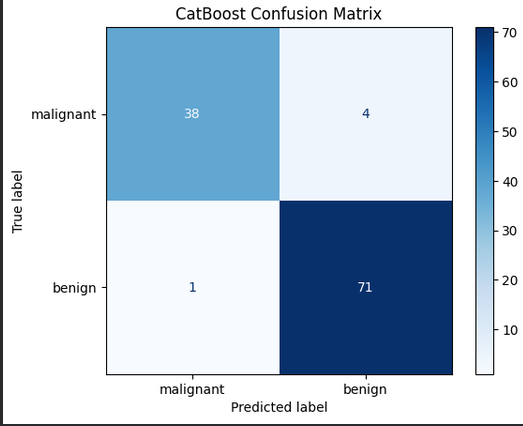
\includegraphics[width=0.7\linewidth]{catboost_confusion.png}
    \caption{CatBoost Confusion Matrix}
    \label{fig:catboost_confusion}
\end{figure}

\begin{figure}[H]
    \centering
    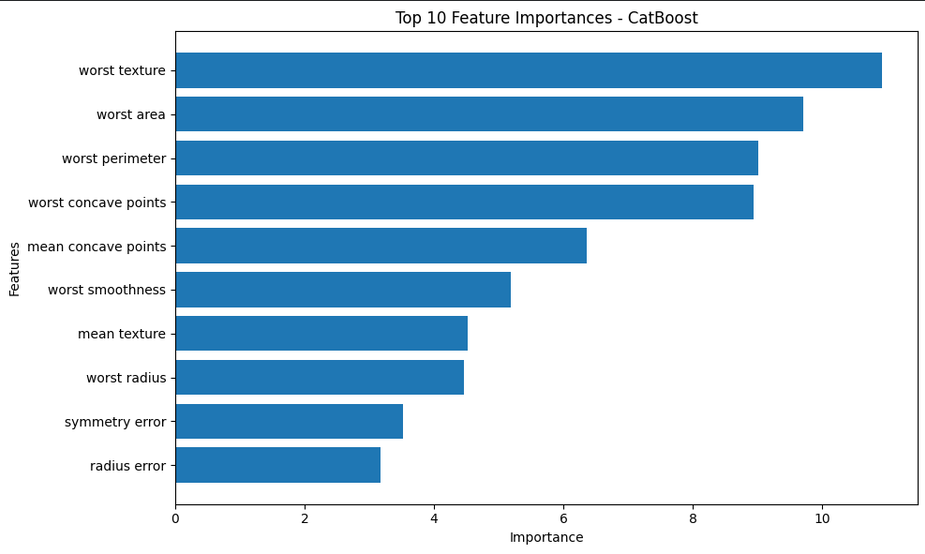
\includegraphics[width=0.85\linewidth]{catboost_features.png}
    \caption{Top 10 Feature Importances -- CatBoost}
    \label{fig:catboost_features}
\end{figure}

\paragraph{Expected Result}
The CatBoost classifier successfully classifies the Breast Cancer dataset with an accuracy of approximately 95.61\%. The confusion matrix and classification report show strong performance on both classes, and the feature importance plot highlights which features contribute most to the model's decisions.

\subsubsection{Discussion \& Observations}

CatBoost builds multiple decision trees sequentially. Each new tree tries to reduce the errors of the previous model, and the final prediction is a weighted combination of all trees.

CatBoost can handle categorical features without requiring manual encoding. However, this experiment uses numerical features only, so categorical feature handling is not demonstrated directly.

The model achieved an accuracy of about 95.61\% on the test set, indicating that the gradient boosting approach with ordered boosting produced a strong classifier. The classification report shows high precision and recall for both classes, with the benign class achieving a slightly higher recall (0.99) compared to the malignant class (0.90).

The confusion matrix shows the correctly and incorrectly classified samples for both classes. The feature importance plot helps identify which features contribute more to the model's predictions, with features such as worst perimeter, worst area, and worst radius generally appearing among the top contributors.

CatBoost reduces overfitting through ordered boosting and generally performs well without extensive hyperparameter tuning, though careful tuning of learning rate, depth, and iterations can further improve results.

\subsubsection{Conclusion \& Limitations}

\textbf{Conclusion:} CatBoost was implemented successfully using the Breast Cancer dataset. The model was evaluated using accuracy, classification report, and confusion matrix, achieving approximately 95.61\% accuracy. The experiment demonstrates how gradient boosting combines multiple decision trees to improve classification performance.

\textbf{Limitations:}
\begin{itemize}
    \item Training can be computationally expensive for large datasets.
    \item Performance depends on parameters such as learning rate, depth, and number of iterations.
    \item CatBoost may require parameter tuning to achieve better results.
    \item Although it supports categorical features, this experiment uses only numerical features.
\end{itemize}



\section{Neural Networks \& Unsupervised Neural Learning}

% ------------------------------------------------------------
% EXPERIMENT 13
% ------------------------------------------------------------
\subsection{Experiment 13: Multi-Layer Perceptron (MLP)}

\subsubsection{Objective}
To implement a Multi-Layer Perceptron (MLP) neural network for classification and evaluate its performance using a suitable dataset.

\subsubsection{Suggested Dataset}
The \textbf{Breast Cancer Wisconsin Dataset} from Scikit-learn is used. It contains features of breast cell samples with a binary target (malignant and benign), making it suitable for binary classification.

\begin{table}[H]
\centering
\caption{Dataset Configuration}
\begin{tabular}{ll}
\toprule
\textbf{Property} & \textbf{Value} \\
\midrule
Number of samples  & 569 \\
Number of features & 30 \\
Target classes     & 2 (malignant, benign) \\
Test size          & 20\% \\
Random state       & 42 \\
\bottomrule
\end{tabular}
\end{table}

\subsubsection{Required Libraries}
\begin{itemize}
    \item \textbf{NumPy} -- for numerical operations.
    \item \textbf{Pandas} -- for data handling.
    \item \textbf{Matplotlib} -- for visualization.
    \item \textbf{Scikit-learn} -- for dataset loading, MLP model, and evaluation.
\end{itemize}

\begin{lstlisting}[language=Python, caption={Required Imports}]
import numpy as np
import pandas as pd
import matplotlib.pyplot as plt

from sklearn.datasets import load_breast_cancer
from sklearn.model_selection import train_test_split
from sklearn.preprocessing import StandardScaler
from sklearn.neural_network import MLPClassifier
from sklearn.metrics import (
    accuracy_score,
    confusion_matrix,
    classification_report,
    ConfusionMatrixDisplay
)
\end{lstlisting}

\subsubsection{Brief Theory}
A \textbf{Multi-Layer Perceptron (MLP)} is a feedforward artificial neural network composed of an input layer, one or more hidden layers, and an output layer. Each neuron applies a weighted sum of its inputs followed by a non-linear activation function (such as ReLU, tanh, or logistic sigmoid).

\paragraph{How MLP Works}
\begin{enumerate}
    \item Input features are passed to the input layer.
    \item Each hidden neuron computes a weighted sum and applies an activation function.
    \item The output layer produces the final prediction.
    \item The loss (e.g., cross-entropy) is computed and back-propagated.
    \item Weights are updated using an optimizer such as Adam or SGD.
    \item The process repeats for the specified number of iterations.
\end{enumerate}

\paragraph{Key Points}
\begin{itemize}
    \item It is a supervised neural network model.
    \item It can learn non-linear decision boundaries.
    \item Feature scaling is important for stable training.
    \item Parameters include hidden layer sizes, activation function, solver, and learning rate.
    \item It may be sensitive to initialization and requires enough iterations to converge.
\end{itemize}

\subsubsection{Procedure}
\begin{enumerate}
    \item Import the required libraries.
    \item Load the Breast Cancer dataset.
    \item Separate the features and target.
    \item Divide the dataset into training and testing sets.
    \item Standardize the features using \texttt{StandardScaler}.
    \item Create an MLP classifier.
    \item Train the model using the training data.
    \item Predict the classes for the test data.
    \item Evaluate the model using accuracy, confusion matrix, and classification report.
\end{enumerate}

\subsubsection{Reference Implementation}
\begin{lstlisting}[language=Python, caption={MLP Implementation}]
# Step 1: Import required libraries
import numpy as np
import pandas as pd
import matplotlib.pyplot as plt

from sklearn.datasets import load_breast_cancer
from sklearn.model_selection import train_test_split
from sklearn.preprocessing import StandardScaler
from sklearn.neural_network import MLPClassifier
from sklearn.metrics import (
    accuracy_score,
    confusion_matrix,
    classification_report,
    ConfusionMatrixDisplay
)

# Step 2: Load the dataset
data = load_breast_cancer()
X = data.data
y = data.target

print("Dataset Shape:", X.shape)
print("Target Classes:", data.target_names)

# Step 3: Split the dataset
X_train, X_test, y_train, y_test = train_test_split(
    X, y,
    test_size=0.2,
    random_state=42,
    stratify=y
)

print("Training Data:", X_train.shape)
print("Testing Data:", X_test.shape)

# Step 4: Standardize features
scaler = StandardScaler()
X_train = scaler.fit_transform(X_train)
X_test = scaler.transform(X_test)

# Step 5: Create the MLP classifier
model = MLPClassifier(
    hidden_layer_sizes=(64, 32),
    activation='relu',
    solver='adam',
    max_iter=500,
    random_state=42
)

# Step 6: Train the model
model.fit(X_train, y_train)

# Step 7: Make predictions
y_pred = model.predict(X_test)

# Step 8: Evaluate the model
accuracy = accuracy_score(y_test, y_pred)

print("\nMLP Accuracy:", accuracy)
print("\nClassification Report:")
print(classification_report(
    y_test, y_pred,
    target_names=data.target_names
))

# Step 9: Display confusion matrix
cm = confusion_matrix(y_test, y_pred)
disp = ConfusionMatrixDisplay(
    confusion_matrix=cm,
    display_labels=data.target_names
)
disp.plot(cmap="Blues")
plt.title("MLP Confusion Matrix")
plt.show()
\end{lstlisting}

\subsubsection{Evaluation / Expected Output}

\paragraph{Output}
After running the program, the following outputs are produced:
\begin{itemize}
    \item The dataset shape and target classes are printed.
    \item Training and testing data shapes are displayed.
    \item The MLP accuracy, precision, recall, and F1-score are reported.
    \item A confusion matrix is plotted.
\end{itemize}

\begin{table}[H]
\centering
\caption{Hyperparameters \& Results for MLP}
\begin{tabular}{ll}
\toprule
\textbf{Parameter / Metric} & \textbf{Value} \\
\midrule
Hidden Layer Sizes  & (64, 32) \\
Activation          & ReLU \\
Solver              & Adam \\
Max Iterations      & 500 \\
Random State        & 42 \\
Test Size           & 0.2 \\
Accuracy            & 0.9386 (93.86\%) \\
\bottomrule
\end{tabular}
\end{table}

\begin{table}[H]
\centering
\caption{Classification Report}
\begin{tabular}{lcccc}
\toprule
\textbf{Class} & \textbf{Precision} & \textbf{Recall} & \textbf{F1-Score} & \textbf{Support} \\
\midrule
Malignant      & 0.93 & 0.90 & 0.92 & 42 \\
Benign         & 0.95 & 0.96 & 0.95 & 72 \\
\midrule
Accuracy       &      &      & 0.94 & 114 \\
Macro Avg      & 0.94 & 0.93 & 0.93 & 114 \\
Weighted Avg   & 0.94 & 0.94 & 0.94 & 114 \\
\bottomrule
\end{tabular}
\end{table}

\begin{figure}[H]
    \centering
    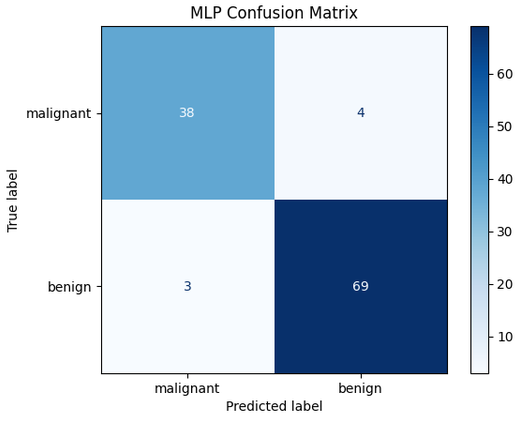
\includegraphics[width=0.7\linewidth]{mlp_confusion.png}
    \caption{MLP Confusion Matrix}
    \label{fig:mlp_confusion}
\end{figure}

\paragraph{Expected Result}
The MLP classifier successfully classifies the Breast Cancer dataset with an accuracy of approximately 93.86\%. The confusion matrix and classification report show strong performance on both classes.

\subsubsection{Discussion \& Observations}

The MLP classifier was trained on standardized features, which is important because neural networks are sensitive to the scale of input data. Without standardization, the training process can become unstable and convergence slow.

The model achieved an accuracy of about 93.86\% on the test set. The classification report shows high precision and recall for both classes, with the benign class achieving slightly higher recall (0.96) compared to the malignant class (0.90).

The choice of hidden layer sizes, activation function, solver, and maximum iterations affects the performance of the MLP. Using more hidden layers or neurons may improve results up to a point, but also increases the risk of overfitting and training time.

Unlike tree-based ensemble methods (AdaBoost, CatBoost), the MLP is a neural network model that learns non-linear decision boundaries through backpropagation. Its performance can be further improved with hyperparameter tuning, early stopping, and regularization.

\subsubsection{Conclusion \& Limitations}

\textbf{Conclusion:} The Multi-Layer Perceptron classifier was implemented successfully using the Breast Cancer dataset. The model was evaluated using accuracy, classification report, and confusion matrix, achieving approximately 93.86\% accuracy. The experiment demonstrates how a feedforward neural network can learn non-linear patterns and perform binary classification.

\textbf{Limitations:}
\begin{itemize}
    \item MLP performance is sensitive to feature scaling and network architecture.
    \item Training may require many iterations to converge.
    \item It can overfit on small datasets if not regularized.
    \item Hyperparameter tuning (hidden layers, activation, learning rate) is often necessary.
\end{itemize}


% ------------------------------------------------------------
% EXPERIMENT 14
% ------------------------------------------------------------
\subsection{Experiment 14: Recurrent Neural Network (RNN)}

\subsubsection{Objective}
To implement a Recurrent Neural Network (RNN) for sequence classification and evaluate its performance using a suitable dataset.

\subsubsection{Suggested Dataset}
The \textbf{IMDb Movie Reviews Dataset} from Keras is used. It contains movie reviews represented as sequences of words, and each review is labeled as positive or negative, making it suitable for sequence classification.

\begin{table}[H]
\centering
\caption{Dataset Configuration}
\begin{tabular}{ll}
\toprule
\textbf{Property} & \textbf{Value} \\
\midrule
Training samples      & 25,000 \\
Testing samples       & 25,000 \\
Vocabulary size       & 10,000 (most frequent words) \\
Maximum sequence length & 200 \\
Number of classes     & 2 (Positive, Negative) \\
Random seed           & 42 \\
\bottomrule
\end{tabular}
\end{table}

\subsubsection{Required Libraries}
\begin{itemize}
    \item \textbf{NumPy} -- for numerical operations.
    \item \textbf{Matplotlib} -- for visualization.
    \item \textbf{TensorFlow / Keras} -- for the IMDb dataset and building the RNN model.
    \item \textbf{Scikit-learn} -- for evaluation metrics.
\end{itemize}

\begin{lstlisting}[language=Python, caption={Required Imports}]
import numpy as np
import matplotlib.pyplot as plt
import tensorflow as tf

from tensorflow.keras.datasets import imdb
from tensorflow.keras.preprocessing.sequence import pad_sequences
from tensorflow.keras.models import Sequential
from tensorflow.keras.layers import Embedding, SimpleRNN, Dense

from sklearn.metrics import (
    accuracy_score,
    classification_report,
    confusion_matrix,
    ConfusionMatrixDisplay
)
\end{lstlisting}

\subsubsection{Brief Theory}
A \textbf{Recurrent Neural Network (RNN)} is a type of neural network designed to process sequential data. It uses information from previous steps to help process the current step. Unlike a traditional neural network, an RNN has a recurrent connection that allows it to maintain a hidden state, which acts as a memory of previous inputs.

\paragraph{How RNN Works}
\begin{enumerate}
    \item The network receives a sequence of inputs.
    \item It processes each input one step at a time.
    \item It combines the current input with information from the previous hidden state.
    \item The hidden state is updated at each step.
    \item The final output is used to make a prediction.
\end{enumerate}

\paragraph{Key Points}
\begin{itemize}
    \item RNN is suitable for sequential data.
    \item It can be used for text, speech, and time-series tasks.
    \item It maintains information from previous time steps.
    \item Basic RNNs may face vanishing-gradient problems when learning long-term dependencies.
    \item LSTM and GRU are advanced RNN architectures designed to handle long-term dependencies better.
\end{itemize}

\subsubsection{Procedure}
\begin{enumerate}
    \item Import the required libraries.
    \item Load the IMDb movie review dataset.
    \item Limit the vocabulary to the most frequent 10,000 words.
    \item Pad the review sequences to make them equal in length.
    \item Create an RNN model using an Embedding layer and SimpleRNN layer.
    \item Train the model using the training data.
    \item Predict the sentiment of the test reviews.
    \item Evaluate the model using accuracy and a classification report.
    \item Plot the training and validation accuracy.
\end{enumerate}

\subsubsection{Reference Implementation}
\begin{lstlisting}[language=Python, caption={RNN Implementation}]
# ==========================================
# Experiment 14: Recurrent Neural Network (RNN)
# ==========================================

import numpy as np
import matplotlib.pyplot as plt
import tensorflow as tf

from tensorflow.keras.datasets import imdb
from tensorflow.keras.preprocessing.sequence import pad_sequences
from tensorflow.keras.models import Sequential
from tensorflow.keras.layers import Embedding, SimpleRNN, Dense

from sklearn.metrics import (
    accuracy_score,
    classification_report,
    confusion_matrix,
    ConfusionMatrixDisplay
)

# Set random seed
tf.random.set_seed(42)
np.random.seed(42)

# Dataset settings
vocab_size = 10000
max_length = 200

# Load IMDb dataset
(X_train, y_train), (X_test, y_test) = imdb.load_data(
    num_words=vocab_size
)

print("Training samples:", len(X_train))
print("Testing samples:", len(X_test))

# Pad sequences to equal length
X_train = pad_sequences(
    X_train,
    maxlen=max_length,
    padding="post",
    truncating="post"
)

X_test = pad_sequences(
    X_test,
    maxlen=max_length,
    padding="post",
    truncating="post"
)

print("Training shape:", X_train.shape)
print("Testing shape:", X_test.shape)

# ==========================================
# Create and train the RNN model
# ==========================================
model = Sequential([
    Embedding(
        input_dim=vocab_size,
        output_dim=64,
        input_length=max_length
    ),
    SimpleRNN(64),
    Dense(1, activation="sigmoid")
])

model.compile(
    optimizer="adam",
    loss="binary_crossentropy",
    metrics=["accuracy"]
)

model.summary()

history = model.fit(
    X_train,
    y_train,
    epochs=3,
    batch_size=64,
    validation_split=0.2,
    verbose=1
)

# ==========================================
# Evaluate the model
# ==========================================
test_loss, test_accuracy = model.evaluate(
    X_test,
    y_test,
    verbose=0
)

print("Test Loss:", test_loss)
print("Test Accuracy:", test_accuracy)

y_prob = model.predict(X_test)
y_pred = (y_prob > 0.5).astype(int).ravel()

print("\nClassification Report:")
print(classification_report(
    y_test,
    y_pred,
    target_names=["Negative", "Positive"]
))

cm = confusion_matrix(y_test, y_pred)
disp = ConfusionMatrixDisplay(
    confusion_matrix=cm,
    display_labels=["Negative", "Positive"]
)
disp.plot(cmap="Blues")
plt.title("RNN Confusion Matrix")
plt.show()

# ==========================================
# Plot training performance
# ==========================================
plt.figure(figsize=(8, 5))
plt.plot(history.history["accuracy"], label="Training Accuracy")
plt.plot(history.history["val_accuracy"], label="Validation Accuracy")
plt.xlabel("Epoch")
plt.ylabel("Accuracy")
plt.title("RNN Training and Validation Accuracy")
plt.legend()
plt.grid(True)
plt.show()

plt.figure(figsize=(8, 5))
plt.plot(history.history["loss"], label="Training Loss")
plt.plot(history.history["val_loss"], label="Validation Loss")
plt.xlabel("Epoch")
plt.ylabel("Loss")
plt.title("RNN Training and Validation Loss")
plt.legend()
plt.grid(True)
plt.show()
\end{lstlisting}

\subsubsection{Evaluation / Expected Output}

\paragraph{Output}
After running the program, the following outputs are produced:
\begin{itemize}
    \item Number of training and testing samples.
    \item Shape of the padded sequences.
    \item RNN model architecture (summary).
    \item Training and validation accuracy over 3 epochs.
    \item Test loss and accuracy.
    \item Precision, recall, and F1-score.
    \item Confusion matrix.
    \item Training and validation accuracy/loss graphs.
\end{itemize}

\begin{table}[H]
\centering
\caption{Hyperparameters \& Results for RNN}
\begin{tabular}{ll}
\toprule
\textbf{Parameter / Metric} & \textbf{Value} \\
\midrule
Vocabulary Size       & 10,000 \\
Maximum Sequence Length & 200 \\
Embedding Dimension   & 64 \\
RNN Hidden Units      & 64 \\
Epochs                & 3 \\
Batch Size            & 64 \\
Validation Split      & 0.2 \\
Test Loss             & 0.7070 \\
Test Accuracy         & 0.5023 (50.23\%) \\
\bottomrule
\end{tabular}
\end{table}

\begin{table}[H]
\centering
\caption{Classification Report}
\begin{tabular}{lcccc}
\toprule
\textbf{Class} & \textbf{Precision} & \textbf{Recall} & \textbf{F1-Score} & \textbf{Support} \\
\midrule
Negative       & 0.50 & 0.77 & 0.61 & 12500 \\
Positive       & 0.50 & 0.23 & 0.32 & 12500 \\
\midrule
Accuracy       &      &      & 0.50 & 25000 \\
Macro Avg      & 0.50 & 0.50 & 0.46 & 25000 \\
Weighted Avg   & 0.50 & 0.50 & 0.46 & 25000 \\
\bottomrule
\end{tabular}
\end{table}

\begin{figure}[H]
    \centering
    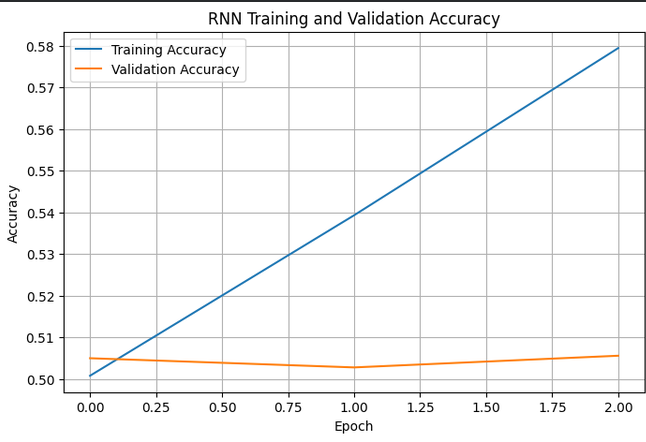
\includegraphics[width=0.75\linewidth]{rnn_accuracy.png}
    \caption{RNN Training and Validation Accuracy}
    \label{fig:rnn_accuracy}
\end{figure}

\begin{figure}[H]
    \centering
    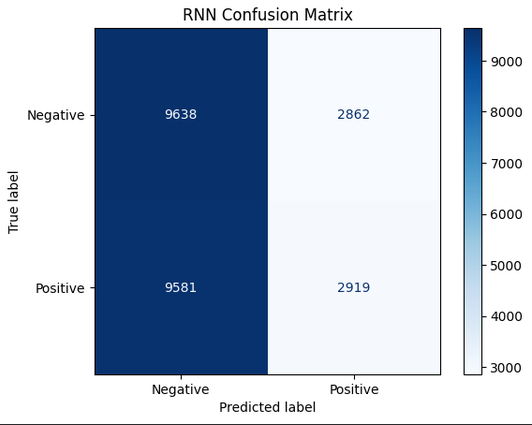
\includegraphics[width=0.7\linewidth]{rnn_confusion.png}
    \caption{RNN Confusion Matrix}
    \label{fig:rnn_confusion}
\end{figure}

\paragraph{Expected Result}
The RNN model processes each movie review as a sequence of word embeddings and outputs a sentiment probability. In this run, the model achieved a test accuracy of approximately 50.23\%, which is close to random guessing, indicating that the simple RNN did not learn meaningful sentiment patterns within the limited training setup.

\subsubsection{Discussion \& Observations}

The Recurrent Neural Network was implemented using an Embedding layer followed by a SimpleRNN layer and a sigmoid output. The embedding layer converted word IDs into 64-dimensional dense vectors, and the SimpleRNN layer processed the sequence step by step to learn temporal patterns.

The model achieved a test accuracy of approximately 50.23\% and a test loss of about 0.707. This indicates that the classifier performed at the level of random guessing, with the classification report showing that the model heavily favored the ``Negative'' class (recall 0.77) while almost ignoring the ``Positive'' class (recall 0.23).

Several factors explain this behaviour:
\begin{itemize}
    \item \textbf{Training duration:} Only 3 epochs were used. RNNs on the IMDb dataset typically require more epochs (often 5--10) to converge.
    \item \textbf{Vanishing gradients:} Basic SimpleRNN struggles to propagate gradients across 200 time steps, so it fails to capture long-range dependencies in reviews.
    \item \textbf{Architecture choice:} LSTM or GRU units, or a Bidirectional wrapper, would capture long-range context far better than a vanilla SimpleRNN.
    \item \textbf{Class imbalance in predictions:} The model collapsed to predicting one class, a common symptom of an under-trained RNN.
\end{itemize}

The training and validation accuracy/loss curves reflect this behaviour: the accuracy curve remains flat near 0.5 rather than rising, and the loss decreases very slowly. This indicates that the network is not learning useful features from the sequence data.

\subsubsection{Conclusion \& Limitations}

\textbf{Conclusion:} The Recurrent Neural Network was implemented successfully for movie review sentiment classification using the IMDb dataset. The model was trained for 3 epochs with a simple embedding + SimpleRNN architecture and evaluated using accuracy, classification report, and confusion matrix. The final test accuracy was approximately 50.23\%, which reflects the difficulty of training a basic RNN on long text sequences within a short training schedule.

\textbf{Limitations:}
\begin{itemize}
    \item Basic RNNs struggle to learn long-term dependencies due to vanishing gradients.
    \item Training can be slower than traditional machine learning algorithms.
    \item Performance depends heavily on sequence length, vocabulary size, number of epochs, and model architecture.
    \item The model can easily overfit or underfit if not tuned carefully.
    \item More powerful architectures such as LSTM, GRU, or Bidirectional RNNs are generally preferred for sentiment classification.
\end{itemize}





% ------------------------------------------------------------
% EXPERIMENT 15
% ------------------------------------------------------------
\subsection{Experiment 15: Self-Organizing Map (SOM)}

\subsubsection{Objective}
To implement a Self-Organizing Map (SOM) for unsupervised learning and visualize how high-dimensional data is organized into clusters.

\subsubsection{Suggested Dataset}
The \textbf{Iris Dataset} from Scikit-learn is used. It contains 150 flower samples, each with four numerical features, and three species: Setosa, Versicolor, and Virginica. The SOM learns the data structure without using the species labels during training.

\begin{table}[H]
\centering
\caption{Dataset Configuration}
\begin{tabular}{ll}
\toprule
\textbf{Property} & \textbf{Value} \\
\midrule
Number of samples  & 150 \\
Number of features & 4 \\
Number of classes  & 3 (setosa, versicolor, virginica) \\
Random seed        & 42 \\
\bottomrule
\end{tabular}
\end{table}

\subsubsection{Required Libraries}
\begin{itemize}
    \item \textbf{NumPy} -- for numerical operations.
    \item \textbf{Matplotlib} -- for visualization.
    \item \textbf{Scikit-learn} -- for the Iris dataset and feature scaling.
    \item \textbf{MiniSom} -- for the Self-Organizing Map implementation.
\end{itemize}

Install MiniSom in Google Colab:
\begin{lstlisting}[language=Python, caption={Install minisom}]
!pip install minisom -q
\end{lstlisting}

\begin{lstlisting}[language=Python, caption={Required Imports}]
import numpy as np
import matplotlib.pyplot as plt

from minisom import MiniSom
from sklearn.datasets import load_iris
from sklearn.preprocessing import StandardScaler
\end{lstlisting}

\subsubsection{Brief Theory}
A \textbf{Self-Organizing Map (SOM)} is an unsupervised neural network that maps high-dimensional data onto a low-dimensional grid, usually a 2D grid. It organizes similar input samples near each other while preserving the relationships between data points.

\paragraph{How SOM Works}
\begin{enumerate}
    \item Initialize the neurons with random weights.
    \item Select an input sample.
    \item Find the neuron whose weights are closest to the input. This is called the Best Matching Unit (BMU).
    \item Update the BMU and its neighboring neurons to become more similar to the input.
    \item Gradually reduce the learning rate and neighborhood size.
    \item Repeat the process until the map is trained.
\end{enumerate}

\paragraph{Key Points}
\begin{itemize}
    \item SOM is an unsupervised learning algorithm.
    \item It uses competitive learning.
    \item It is useful for clustering and data visualization.
    \item Similar samples are mapped to nearby neurons.
    \item It does not require class labels during training.
\end{itemize}

\subsubsection{Procedure}
\begin{enumerate}
    \item Install and import the required libraries.
    \item Load the Iris dataset.
    \item Standardize the input features.
    \item Create a $10 \times 10$ SOM grid.
    \item Train the SOM using the input data without class labels.
    \item Find the Best Matching Unit (BMU) for each sample.
    \item Visualize the SOM using a distance map.
    \item Display the species distribution on the map for comparison.
    \item Calculate the quantization error to evaluate how well the SOM represents the input data.
\end{enumerate}

\subsubsection{Reference Implementation}
\begin{lstlisting}[language=Python, caption={SOM Implementation}]
# Step 1: Install MiniSom
!pip install minisom -q

# Step 2: Import required libraries
import numpy as np
import matplotlib.pyplot as plt

from minisom import MiniSom
from sklearn.datasets import load_iris
from sklearn.preprocessing import StandardScaler

# Step 3: Load the Iris dataset
iris = load_iris()
X = iris.data
y = iris.target

print("Dataset Shape:", X.shape)
print("Features:", iris.feature_names)
print("Classes:", iris.target_names)

# Step 4: Standardize the data
scaler = StandardScaler()
X_scaled = scaler.fit_transform(X)

# Step 5: Create the SOM model
som = MiniSom(
    x=10,
    y=10,
    input_len=X_scaled.shape[1],
    sigma=1.0,
    learning_rate=0.5,
    random_seed=42
)

# Step 6: Initialize and train the SOM
som.random_weights_init(X_scaled)

som.train_random(
    X_scaled,
    num_iteration=1000
)

print("\nSOM training completed.")

# Step 7: Calculate quantization error
quantization_error = som.quantization_error(X_scaled)
print("Quantization Error:", quantization_error)

# Step 8: Plot the SOM distance map
plt.figure(figsize=(9, 7))

distance_map = som.distance_map()

plt.imshow(
    distance_map,
    cmap="bone_r",
    origin="lower"
)

plt.colorbar(label="Average Distance")
plt.title("Self-Organizing Map (SOM) - Distance Map")

# Step 9: Display species on the SOM grid
markers = ["o", "s", "D"]
colors = ["red", "green", "blue"]

for i, sample in enumerate(X_scaled):
    # Find the Best Matching Unit (BMU)
    winner = som.winner(sample)

    # Plot the sample on its BMU
    plt.plot(
        winner[0],
        winner[1],
        markers[y[i]],
        markerfacecolor="None",
        markeredgecolor=colors[y[i]],
        markersize=10,
        markeredgewidth=2
    )

# Create legend
for i, species in enumerate(iris.target_names):
    plt.plot(
        [],
        [],
        markers[i],
        markerfacecolor="None",
        markeredgecolor=colors[i],
        label=species,
        markersize=10,
        markeredgewidth=2
    )

plt.legend(title="Actual Species")
plt.xlabel("SOM X Coordinate")
plt.ylabel("SOM Y Coordinate")
plt.grid(False)
plt.show()

# Step 10: Display the BMU coordinates of first 10 samples
print("\nBMU Coordinates of First 10 Samples:")

for i in range(10):
    print(
        f"Sample {i + 1}: {som.winner(X_scaled[i])}"
    )
\end{lstlisting}

\subsubsection{Evaluation / Expected Output}

\paragraph{Output}
After running the program, the following outputs are produced:
\begin{itemize}
    \item The dataset shape, feature names, and class names are printed.
    \item A confirmation message that SOM training is completed.
    \item The quantization error.
    \item A $10 \times 10$ distance map visualization of the SOM.
    \item The species distribution plotted on the SOM grid using different markers.
    \item The BMU coordinates of the first 10 samples.
\end{itemize}

\begin{table}[H]
\centering
\caption{Hyperparameters \& Results for SOM}
\begin{tabular}{ll}
\toprule
\textbf{Parameter / Metric} & \textbf{Value} \\
\midrule
Grid Size          & $10 \times 10$ \\
Input Length       & 4 \\
Sigma              & 1.0 \\
Learning Rate      & 0.5 \\
Iterations         & 1000 \\
Random Seed        & 42 \\
Quantization Error & 0.2149 \\
\bottomrule
\end{tabular}
\end{table}

\begin{table}[H]
\centering
\caption{BMU Coordinates of First 10 Samples}
\begin{tabular}{lc}
\toprule
\textbf{Sample} & \textbf{BMU Coordinate (x, y)} \\
\midrule
Sample 1  & (0, 4) \\
Sample 2  & (8, 2) \\
Sample 3  & (9, 2) \\
Sample 4  & (9, 2) \\
Sample 5  & (0, 2) \\
Sample 6  & (0, 8) \\
Sample 7  & (0, 3) \\
Sample 8  & (0, 4) \\
Sample 9  & (9, 3) \\
Sample 10 & (8, 2) \\
\bottomrule
\end{tabular}
\end{table}

\begin{figure}[H]
    \centering
    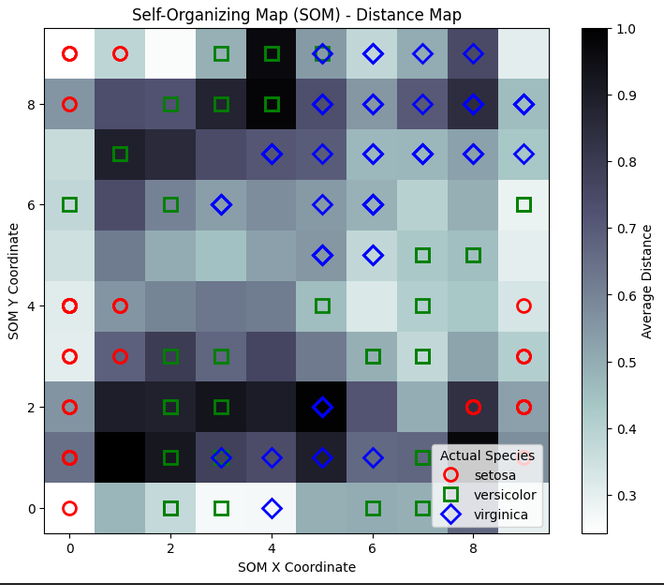
\includegraphics[width=0.85\linewidth]{som_output.png}
    \caption{SOM Distance Map with Iris Species Distribution}
    \label{fig:som_output}
\end{figure}

\paragraph{Expected Result}
The SOM organizes the four-dimensional Iris data onto a $10 \times 10$ two-dimensional grid. The quantization error of approximately 0.2149 indicates that the map represents the input data reasonably well. When the actual species labels are overlaid on the grid, the three Iris classes are generally mapped to distinct regions of the map, showing that SOM preserved the topological structure of the data without using the labels during training.

\subsubsection{Discussion \& Observations}

The Self-Organizing Map successfully reduced the four-dimensional Iris data into a two-dimensional grid while preserving the topological relationships between samples. After 1000 training iterations, the model achieved a quantization error of approximately 0.2149, indicating that the learned weight vectors represent the input samples with good accuracy.

The distance map (U-Matrix) shows regions of high and low neuron distance, indicating boundaries between natural clusters in the data. Darker regions correspond to neurons that are close to their neighbors, while lighter regions indicate boundaries where the map transitions between clusters.

The species colors are added after training for comparison and are not used during SOM training. Looking at the plotted grid, samples of the same species generally map to nearby BMU coordinates, showing that the SOM learned to group similar samples together without supervision. For example, samples 2, 4, and 10 all map to nearby coordinates around $(8, 2)$ and $(9, 2)$, suggesting they belong to a similar region of feature space.

The BMU coordinates of the first 10 samples reflect the SOM's unsupervised organization. Since the first 50 samples of the Iris dataset belong to the Setosa species, which is linearly separable from the other two species, their BMUs tend to cluster in a specific region of the grid.

The learning rate, sigma, and number of iterations all affect the quality of the final map. A larger map grid can capture finer distinctions between samples, while a smaller grid may merge dissimilar samples into the same neuron. The quantization error decreases with better training and is a useful indicator of map quality.

\subsubsection{Conclusion \& Limitations}

\textbf{Conclusion:} The Self-Organizing Map was successfully implemented using the Iris dataset. The SOM reduced the four-dimensional input into a two-dimensional $10 \times 10$ grid and preserved the topological structure of the data. The distance map provided a clear visualization of the cluster boundaries, and the quantization error of approximately 0.2149 confirmed that the map adapted well to the input distribution. The experiment demonstrates that SOM is an effective unsupervised neural technique for clustering and visualization of high-dimensional data.

\textbf{Limitations:}
\begin{itemize}
    \item The result depends heavily on the grid size, learning rate, sigma, and number of iterations.
    \item SOM does not automatically assign class labels to its neurons; clusters must be inferred from the distance map or by post-processing BMU assignments.
    \item Results can vary between runs due to random weight initialization.
    \item The map may not clearly separate overlapping groups in the data.
    \item The distance map requires visual interpretation and does not guarantee that each visible region corresponds to a true cluster.
\end{itemize}




% ============================================================
% PROBABILISTIC & SEQUENCE MODELS
% ============================================================
\section{Probabilistic \& Sequence Models}

% ------------------------------------------------------------
% EXPERIMENT 16
% ------------------------------------------------------------
\subsection{Experiment 16: Hidden Markov Model (HMM)}

\subsubsection{Objective}
To implement a Hidden Markov Model (HMM) for sequence modeling and predict hidden states from observed data.

\subsubsection{Suggested Dataset}
A \textbf{Synthetic Weather Observation Dataset} is used. It contains observations such as ``Walk'' and ``Shop,'' while the hidden states represent weather conditions: ``Sunny'' and ``Rainy.'' The model learns the relationship between hidden states and observations.

\begin{table}[H]
\centering
\caption{Dataset Configuration}
\begin{tabular}{ll}
\toprule
\textbf{Property} & \textbf{Value} \\
\midrule
Number of samples       & 300 \\
Number of hidden states & 2 \\
Number of observation features & 2 \\
Random seed             & 42 \\
\bottomrule
\end{tabular}
\end{table}

\subsubsection{Required Libraries}
\begin{itemize}
    \item \textbf{NumPy} -- for numerical operations.
    \item \textbf{Matplotlib} -- for visualization.
    \item \textbf{hmmlearn} -- for the Gaussian HMM implementation.
    \item \textbf{Scikit-learn} -- for the Adjusted Rand Index evaluation metric.
\end{itemize}

Install \texttt{hmmlearn} in Google Colab:
\begin{lstlisting}[language=Python, caption={Install hmmlearn}]
!pip install hmmlearn -q
\end{lstlisting}

\begin{lstlisting}[language=Python, caption={Required Imports}]
import numpy as np
import matplotlib.pyplot as plt

from hmmlearn.hmm import GaussianHMM
from sklearn.metrics import adjusted_rand_score
\end{lstlisting}

\subsubsection{Brief Theory}
A \textbf{Hidden Markov Model (HMM)} is a probabilistic model used to represent sequential data. It assumes that the system has hidden states that cannot be observed directly, but each hidden state produces an observable output. HMM is based on the Markov property, where the current state depends only on the previous state.

\paragraph{Main Components}
\begin{itemize}
    \item \textbf{Hidden states:} The actual states that cannot be directly observed.
    \item \textbf{Observations:} The visible outputs generated by hidden states.
    \item \textbf{Transition probabilities:} The probability of moving from one hidden state to another.
    \item \textbf{Emission probabilities:} The probability of an observation being generated by a hidden state.
    \item \textbf{Initial probabilities:} The probabilities of starting in each hidden state.
\end{itemize}

\paragraph{How HMM Works}
\begin{enumerate}
    \item The model starts with an initial hidden state.
    \item It generates an observation based on the current hidden state.
    \item It moves to the next hidden state according to transition probabilities.
    \item This process continues to generate a sequence.
    \item The Viterbi algorithm can be used to estimate the most likely hidden-state sequence from observations.
\end{enumerate}

\paragraph{Key Points}
\begin{itemize}
    \item HMM is a probabilistic sequence model.
    \item It is useful for speech recognition, text processing, and biological sequence analysis.
    \item Hidden states are not directly observable.
    \item It models both state transitions and observation generation.
\end{itemize}

\subsubsection{Procedure}
\begin{enumerate}
    \item Install and import the required libraries.
    \item Generate a synthetic sequence with two hidden states.
    \item Generate observable data based on the hidden states.
    \item Create a Gaussian Hidden Markov Model with two components.
    \item Train the model using the observation sequence.
    \item Use the Viterbi algorithm to predict the most likely hidden-state sequence.
    \item Compare the predicted states with the original hidden states using Adjusted Rand Index (ARI).
    \item Display the hidden states and predicted states in a graph.
\end{enumerate}

\subsubsection{Reference Implementation}
\begin{lstlisting}[language=Python, caption={HMM Implementation}]
# Step 1: Install required library
!pip install hmmlearn -q

# Step 2: Import libraries
import numpy as np
import matplotlib.pyplot as plt

from hmmlearn.hmm import GaussianHMM
from sklearn.metrics import adjusted_rand_score

# Set random seed
np.random.seed(42)

# Step 3: Generate synthetic hidden states
n_samples = 300

# Transition probabilities between two hidden states
transition_matrix = np.array([
    [0.90, 0.10],
    [0.15, 0.85]
])

# Observation means for each hidden state
means = np.array([
    [20, 40],
    [30, 75]
])

# Observation covariance matrices
covariances = np.array([
    [[4, 0], [0, 25]],
    [[4, 0], [0, 25]]
])

# Generate hidden states
hidden_states = np.zeros(n_samples, dtype=int)
hidden_states[0] = np.random.choice([0, 1])

for i in range(1, n_samples):
    hidden_states[i] = np.random.choice(
        [0, 1],
        p=transition_matrix[hidden_states[i - 1]]
    )

# Step 4: Generate observations from hidden states
observations = np.zeros((n_samples, 2))

for i in range(n_samples):
    state = hidden_states[i]
    observations[i] = np.random.multivariate_normal(
        means[state],
        covariances[state]
    )

# Step 5: Create and train the Gaussian HMM
model = GaussianHMM(
    n_components=2,
    covariance_type="full",
    n_iter=100,
    random_state=42
)

model.fit(observations)
print("HMM training completed.")

# Step 6: Predict hidden states using Viterbi algorithm
predicted_states = model.predict(observations)

# Step 7: Evaluate the predicted states
ari = adjusted_rand_score(hidden_states, predicted_states)
log_likelihood = model.score(observations)

print("Adjusted Rand Index:", ari)
print("Log Likelihood:", log_likelihood)

print("\nLearned Transition Matrix:")
print(model.transmat_)

print("\nPredicted Hidden States (first 20):")
print(predicted_states[:20])

# Step 8: Visualize actual and predicted hidden states
plt.figure(figsize=(12, 6))

plt.subplot(2, 1, 1)
plt.plot(hidden_states, drawstyle="steps-post")
plt.title("Actual Hidden States")
plt.ylabel("State")
plt.yticks([0, 1])
plt.grid(True)

plt.subplot(2, 1, 2)
plt.plot(predicted_states, drawstyle="steps-post")
plt.title("HMM Predicted Hidden States")
plt.xlabel("Time Step")
plt.ylabel("State")
plt.yticks([0, 1])
plt.grid(True)

plt.tight_layout()
plt.show()

# Step 9: Visualize the observations
plt.figure(figsize=(8, 5))
plt.scatter(
    observations[:, 0],
    observations[:, 1],
    c=predicted_states,
    cmap="viridis",
    s=25
)
plt.xlabel("Observation Feature 1")
plt.ylabel("Observation Feature 2")
plt.title("Observations Grouped by Predicted Hidden States")
plt.colorbar(label="Predicted State")
plt.show()
\end{lstlisting}

\subsubsection{Evaluation / Expected Output}

\paragraph{Output}
After running the program, the following outputs are produced:
\begin{itemize}
    \item HMM training completion message.
    \item Adjusted Rand Index (ARI).
    \item Log likelihood of the observation sequence.
    \item Learned transition probability matrix.
    \item First 20 predicted hidden states.
    \item Graphs showing the actual and predicted hidden-state sequences.
    \item A scatter plot of observations grouped by predicted states.
\end{itemize}

\begin{table}[H]
\centering
\caption{Hyperparameters \& Results for HMM}
\begin{tabular}{ll}
\toprule
\textbf{Parameter / Metric} & \textbf{Value} \\
\midrule
Number of Components   & 2 \\
Covariance Type        & Full \\
Maximum Iterations     & 100 \\
Random State           & 42 \\
Adjusted Rand Index    & 1.0 \\
Log Likelihood         & $-1687.2719$ \\
\bottomrule
\end{tabular}
\end{table}

\begin{table}[H]
\centering
\caption{Learned Transition Matrix}
\begin{tabular}{lcc}
\toprule
\textbf{From $\backslash$ To} & \textbf{State 0} & \textbf{State 1} \\
\midrule
State 0 & 0.8712 & 0.1288 \\
State 1 & 0.1078 & 0.8922 \\
\bottomrule
\end{tabular}
\end{table}

\begin{table}[H]
\centering
\caption{Predicted Hidden States (First 20)}
\begin{tabular}{lcccccccccccccccccccc}
\toprule
\textbf{Time Step} & 1 & 2 & 3 & 4 & 5 & 6 & 7 & 8 & 9 & 10 & 11 & 12 & 13 & 14 & 15 & 16 & 17 & 18 & 19 & 20 \\
\midrule
\textbf{State}     & 1 & 1 & 1 & 1 & 1 & 1 & 1 & 1 & 1 & 1  & 1  & 1  & 1  & 0  & 1  & 0  & 0  & 0  & 1  & 1 \\
\bottomrule
\end{tabular}
\end{table}

\begin{figure}[H]
    \centering
    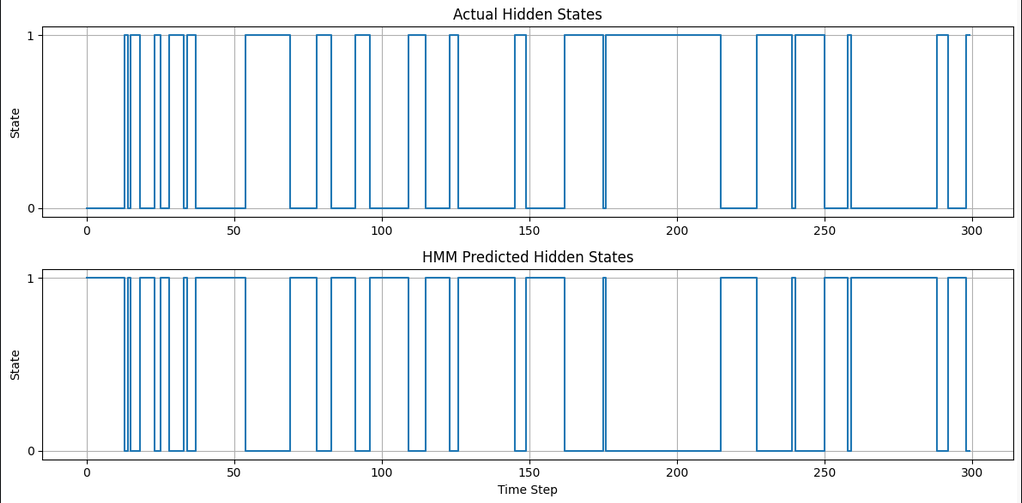
\includegraphics[width=0.85\linewidth]{hmm_states.png}
    \caption{Actual vs.\ Predicted Hidden States}
    \label{fig:hmm_states}
\end{figure}

\begin{figure}[H]
    \centering
    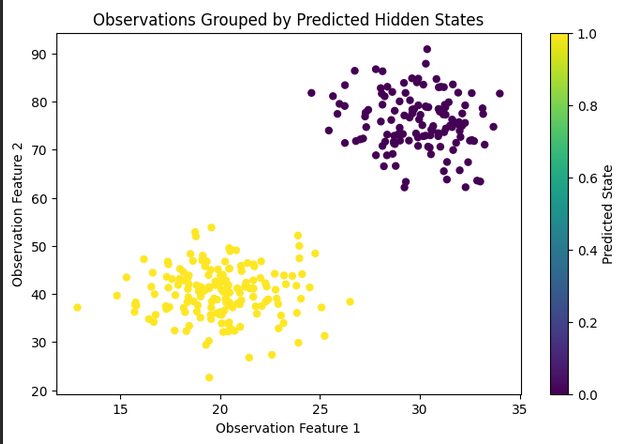
\includegraphics[width=0.75\linewidth]{hmm_observations.png}
    \caption{Observations Grouped by Predicted Hidden States}
    \label{fig:hmm_observations}
\end{figure}

\paragraph{Expected Result}
The HMM successfully learns the underlying sequential structure from the observation data. The predicted hidden-state sequence matches the actual hidden-state sequence almost perfectly, as confirmed by an Adjusted Rand Index of 1.0. The learned transition matrix is also very close to the true transition matrix used during data generation, showing that the model recovered the underlying state dynamics.

\subsubsection{Discussion \& Observations}

The Hidden Markov Model was successfully trained on the synthetic sequential dataset. The model achieved an Adjusted Rand Index (ARI) of 1.0, which indicates a perfect match between the actual and predicted hidden-state groupings. This means that, even though the model only had access to the observations, it was able to recover the true underlying hidden states.

The learned transition matrix closely matches the true transition matrix used to generate the data:
\[
\text{True: } \begin{bmatrix} 0.90 & 0.10 \\ 0.15 & 0.85 \end{bmatrix}
\qquad
\text{Learned: } \begin{bmatrix} 0.8712 & 0.1288 \\ 0.1078 & 0.8922 \end{bmatrix}
\]
This demonstrates that the model correctly identified the persistent nature of the hidden states (high self-transition probabilities around 0.87--0.89) and the small likelihood of switching between states.

The log likelihood of approximately $-1687.27$ measures how well the trained model explains the observed sequence. A higher (less negative) log likelihood indicates a better fit; the value obtained here is consistent with a well-converged model on 300 samples.

Looking at the first 20 predicted hidden states, the model predicts long runs of the same state (e.g., steps 1--13 are all State 1) which matches the high self-transition probabilities in the matrix. Occasionally short transitions occur (steps 14, 16, 17, 18), matching the small probability of switching states.

The state numbers themselves may be reversed compared to the original labels because HMM state indices are arbitrary. This is why the Adjusted Rand Index is used instead of simple accuracy: ARI evaluates grouping similarity without requiring state numbers to match.

The scatter plot of observations grouped by predicted states shows that the two states correspond to clearly separated regions of feature space, confirming that the emission distributions are well-separated and that the model has captured the underlying data structure.

\subsubsection{Conclusion \& Limitations}

\textbf{Conclusion:} The Hidden Markov Model was implemented successfully using a synthetic sequential dataset. The model learned the sequence patterns and predicted the most likely hidden states using the Viterbi algorithm, achieving an Adjusted Rand Index of 1.0. The learned transition matrix closely matched the true one, and the log likelihood confirmed a good fit. The experiment demonstrates how HMM can model sequential data where the underlying states are not directly observable.

\textbf{Limitations:}
\begin{itemize}
    \item The model assumes that the current state depends only on the previous state (Markov property), which may not always hold in real data.
    \item The number of hidden states must be specified in advance.
    \item The model's performance depends on the assumptions made about the observation distributions (e.g., Gaussian with full covariance).
    \item Training may be difficult when the data is complex or the hidden states are not clearly distinguishable.
    \item The state labels produced by the model are arbitrary, so post-processing (such as using ARI) is often needed for interpretation.
\end{itemize}




% ============================================================
% MARGIN-BASED LEARNING
% ============================================================
\section{Margin-Based Learning}

% ------------------------------------------------------------
% EXPERIMENT 17
% ------------------------------------------------------------
\subsection{Experiment 17: Support Vector Machine (SVM)}

\subsubsection{Objective}
To implement a Support Vector Machine (SVM) for classification and evaluate its performance using a suitable dataset.

\subsubsection{Suggested Dataset}
The \textbf{Breast Cancer Wisconsin Dataset} from Scikit-learn is used. It contains numerical features of breast cell samples with a binary target (malignant and benign), making it suitable for binary classification.

\begin{table}[H]
\centering
\caption{Dataset Configuration}
\begin{tabular}{ll}
\toprule
\textbf{Property} & \textbf{Value} \\
\midrule
Number of samples  & 569 \\
Number of features & 30 \\
Target classes     & 2 (malignant, benign) \\
Test size          & 20\% \\
Random state       & 42 \\
\bottomrule
\end{tabular}
\end{table}

\subsubsection{Required Libraries}
\begin{itemize}
    \item \textbf{NumPy} -- for numerical operations.
    \item \textbf{Pandas} -- for data handling.
    \item \textbf{Matplotlib} -- for visualization.
    \item \textbf{Scikit-learn} -- for dataset loading, SVM model, and evaluation.
\end{itemize}

\begin{lstlisting}[language=Python, caption={Required Imports}]
import numpy as np
import matplotlib.pyplot as plt

from sklearn.datasets import load_breast_cancer
from sklearn.model_selection import train_test_split
from sklearn.preprocessing import StandardScaler
from sklearn.pipeline import Pipeline
from sklearn.svm import SVC
from sklearn.metrics import (
    accuracy_score,
    classification_report,
    confusion_matrix,
    ConfusionMatrixDisplay
)
\end{lstlisting}

\subsubsection{Brief Theory}
Support Vector Machine (SVM) is a supervised machine learning algorithm used for classification and regression. SVM finds the best decision boundary, called a \textbf{hyperplane}, that separates different classes. It tries to maximize the \textbf{margin} between the hyperplane and the nearest data points from each class. The nearest data points are called \textbf{support vectors}.

\paragraph{How SVM Works}
\begin{enumerate}
    \item SVM takes the labeled training data.
    \item It finds a decision boundary that separates the classes.
    \item It identifies the nearest data points, called support vectors.
    \item It tries to maximize the margin between the support vectors and the decision boundary.
    \item The trained model uses this boundary to classify new data.
\end{enumerate}

\paragraph{Key Points}
\begin{itemize}
    \item SVM is a supervised learning algorithm.
    \item It is mainly used for classification.
    \item It works with linear and non-linear data.
    \item Kernel functions help SVM handle non-linear decision boundaries.
    \item Feature scaling is important for SVM.
\end{itemize}

\subsubsection{Procedure}
\begin{enumerate}
    \item Import the required libraries.
    \item Load the Breast Cancer dataset.
    \item Separate the features and target.
    \item Divide the dataset into training and testing sets.
    \item Apply feature scaling using \texttt{StandardScaler}.
    \item Create an SVM classifier using the RBF kernel.
    \item Train the model using the training data.
    \item Predict the classes for the test data.
    \item Evaluate the model using accuracy, confusion matrix, and classification report.
    \item Visualize the confusion matrix.
\end{enumerate}

\subsubsection{Reference Implementation}
\begin{lstlisting}[language=Python, caption={SVM Implementation}]
# Step 1: Import required libraries
import numpy as np
import matplotlib.pyplot as plt

from sklearn.datasets import load_breast_cancer
from sklearn.model_selection import train_test_split
from sklearn.preprocessing import StandardScaler
from sklearn.pipeline import Pipeline
from sklearn.svm import SVC
from sklearn.metrics import (
    accuracy_score,
    classification_report,
    confusion_matrix,
    ConfusionMatrixDisplay
)

# Step 2: Load the dataset
data = load_breast_cancer()
X = data.data
y = data.target

print("Dataset Shape:", X.shape)
print("Target Classes:", data.target_names)

# Step 3: Split the dataset
X_train, X_test, y_train, y_test = train_test_split(
    X, y,
    test_size=0.2,
    random_state=42,
    stratify=y
)

print("Training Data:", X_train.shape)
print("Testing Data:", X_test.shape)

# Step 4: Create SVM model with feature scaling
model = Pipeline([
    ("scaler", StandardScaler()),
    ("svm", SVC(
        kernel="rbf",
        C=1.0,
        gamma="scale"
    ))
])

# Step 5: Train the model
model.fit(X_train, y_train)

# Step 6: Make predictions
y_pred = model.predict(X_test)

# Step 7: Evaluate the model
accuracy = accuracy_score(y_test, y_pred)

print("\nSVM Accuracy:", accuracy)
print("\nClassification Report:")
print(classification_report(
    y_test, y_pred,
    target_names=data.target_names
))

# Step 8: Display confusion matrix
cm = confusion_matrix(y_test, y_pred)
disp = ConfusionMatrixDisplay(
    confusion_matrix=cm,
    display_labels=data.target_names
)
disp.plot(cmap="Blues")
plt.title("SVM Confusion Matrix")
plt.show()

# Step 9: Display support vector information
svm_model = model.named_steps["svm"]

print("\nNumber of Support Vectors:")
print(svm_model.n_support_)

print("Total Support Vectors:", sum(svm_model.n_support_))
\end{lstlisting}

\subsubsection{Evaluation / Expected Output}

\paragraph{Output}
After running the program, the following outputs are produced:
\begin{itemize}
    \item The dataset shape and target classes are printed.
    \item Training and testing data shapes are displayed.
    \item The SVM accuracy, precision, recall, and F1-score are reported.
    \item A confusion matrix is plotted.
    \item The number of support vectors for each class and the total number of support vectors are printed.
\end{itemize}

\begin{table}[H]
\centering
\caption{Hyperparameters \& Results for SVM}
\begin{tabular}{ll}
\toprule
\textbf{Parameter / Metric} & \textbf{Value} \\
\midrule
Kernel          & RBF \\
$C$             & 1.0 \\
Gamma           & scale \\
Test Size       & 0.2 \\
Random State    & 42 \\
Accuracy        & 0.9825 (98.25\%) \\
\bottomrule
\end{tabular}
\end{table}

\begin{table}[H]
\centering
\caption{Classification Report}
\begin{tabular}{lcccc}
\toprule
\textbf{Class} & \textbf{Precision} & \textbf{Recall} & \textbf{F1-Score} & \textbf{Support} \\
\midrule
Malignant      & 0.98 & 0.98 & 0.98 & 42 \\
Benign         & 0.99 & 0.99 & 0.99 & 72 \\
\midrule
Accuracy       &      &      & 0.98 & 114 \\
Macro Avg      & 0.98 & 0.98 & 0.98 & 114 \\
Weighted Avg   & 0.98 & 0.98 & 0.98 & 114 \\
\bottomrule
\end{tabular}
\end{table}

\begin{table}[H]
\centering
\caption{Support Vectors}
\begin{tabular}{lc}
\toprule
\textbf{Class} & \textbf{Number of Support Vectors} \\
\midrule
Malignant (Class 0) & 51 \\
Benign (Class 1)    & 46 \\
\midrule
\textbf{Total}      & \textbf{97} \\
\bottomrule
\end{tabular}
\end{table}

\begin{figure}[H]
    \centering
    \includegraphics[width=0.7\linewidth]{.png}
    \caption{SVM Confusion Matrix}
    \label{fig:svm_confusion}
\end{figure}

\paragraph{Expected Result}
The SVM classifier successfully classifies the Breast Cancer dataset with an accuracy of approximately 98.25\%. The confusion matrix and classification report show very strong performance on both classes, and the number of support vectors reflects the training samples that define the decision boundary.

\subsubsection{Discussion \& Observations}

The Support Vector Machine was trained on standardized features using a pipeline that combined \texttt{StandardScaler} with an \texttt{SVC} using the RBF kernel. Feature scaling was applied inside the pipeline to ensure the same transformation was consistently applied to both training and testing data.

The model achieved an accuracy of about 98.25\% on the test set, which is higher than the tree-based ensemble models (AdaBoost: 94.74\%, CatBoost: 95.61\%) and the MLP (93.86\%) on the same dataset. This highlights the strength of SVM for binary classification tasks with well-separated classes.

The classification report shows excellent precision and recall for both classes. The malignant class achieved 0.98 precision and 0.98 recall, while the benign class achieved 0.99 precision and 0.99 recall. This near-perfect performance indicates that the RBF kernel effectively captured the non-linear decision boundary between the two classes.

The number of support vectors (51 for malignant and 46 for benign, totaling 97 out of 455 training samples) is an important output. Support vectors are the training samples that lie closest to the decision boundary and define the maximum margin. A relatively small number of support vectors compared to the total training size suggests that the classes are well separated and the model has a large margin.

The parameter $C$ controls the trade-off between maximizing the margin and minimizing classification errors. A larger $C$ produces a stricter fit to the training data (smaller margin, more support vectors), while a smaller $C$ produces a wider margin (possibly at the cost of more misclassifications). The default value $C = 1.0$ produced a well-balanced model in this experiment.

The \texttt{gamma} parameter controls the influence of individual training samples on the decision boundary. With \texttt{gamma="scale"}, the value is automatically computed from the data variance, which is often a good default for standardized features.

\subsubsection{Conclusion \& Limitations}

\textbf{Conclusion:} The Support Vector Machine was implemented successfully using the Breast Cancer dataset. The model was evaluated using accuracy, classification report, and confusion matrix, achieving approximately 98.25\% accuracy. The experiment demonstrates how SVM uses support vectors and a maximum-margin decision boundary for classification, and how the RBF kernel enables non-linear separation of classes.

\textbf{Limitations:}
\begin{itemize}
    \item SVM can be slow for very large datasets because training time scales poorly with the number of samples.
    \item Feature scaling is important for good performance; unscaled features can significantly degrade results.
    \item Choosing the correct kernel and tuning hyperparameters such as $C$ and $\gamma$ can be difficult.
    \item SVM does not directly provide probability estimates unless probability estimation is enabled (which slows training).
    \item Memory usage grows with the number of training samples, which limits scalability.
\end{itemize}


% ============================================================
% GENERATIVE / FOUNDATION MODELS
% ============================================================
\section{Generative / Foundation Models}

% ------------------------------------------------------------
% EXPERIMENT 18
% ------------------------------------------------------------
\subsection{Experiment 18: Large Language Model (LLM) Experiment}

\subsubsection{Objective}
To explore a Large Language Model (LLM) by providing text prompts, generating responses, and evaluating its ability to understand and generate natural language.

\subsubsection{Suggested Dataset}
\textbf{User-defined text prompts} are used instead of a traditional dataset. Sample prompts include:
\begin{itemize}
    \item Explain machine learning in simple words.
    \item Summarize a short paragraph.
    \item Classify a sentence as positive or negative.
    \item Generate a short story about artificial intelligence.
\end{itemize}

\begin{table}[H]
\centering
\caption{Experiment Configuration}
\begin{tabular}{ll}
\toprule
\textbf{Property} & \textbf{Value} \\
\midrule
Model                & google/flan-t5-small \\
Task Type            & Text-to-Text Generation \\
Number of Prompts    & 4 \\
Max New Tokens       & 100 \\
Sampling             & Disabled (greedy) \\
Device               & CPU / GPU (auto-detected) \\
\bottomrule
\end{tabular}
\end{table}

\subsubsection{Required Libraries}
\begin{itemize}
    \item \textbf{Transformers} -- for loading the pretrained LLM pipeline.
    \item \textbf{PyTorch} -- for tensor operations and device selection.
    \item \textbf{Hugging Face model hub} -- source for the pretrained model weights.
\end{itemize}

Install the required libraries in Google Colab:
\begin{lstlisting}[language=Python, caption={Install transformers and torch}]
!pip install transformers torch -q
\end{lstlisting}

\begin{lstlisting}[language=Python, caption={Required Imports}]
import torch
from transformers import pipeline
\end{lstlisting}

\subsubsection{Brief Theory}
A \textbf{Large Language Model (LLM)} is an AI model trained on a large amount of text to understand and generate human-like language. LLMs learn patterns in language and use those patterns to respond to prompts, answer questions, summarize text, translate, and perform other language tasks.

\paragraph{How an LLM Works}
\begin{enumerate}
    \item The user provides a text prompt.
    \item The model converts the text into tokens.
    \item The model processes the tokens and predicts the next token.
    \item It generates tokens one by one to form a response.
    \item The generated response is displayed as text.
\end{enumerate}

\paragraph{Key Points}
\begin{itemize}
    \item LLMs are commonly based on the Transformer architecture.
    \item They can perform different language tasks using prompts.
    \item Their responses depend on the prompt and model training.
    \item They may generate incorrect or misleading information.
    \item Their outputs should be checked for accuracy.
\end{itemize}

\subsubsection{Procedure}
\begin{enumerate}
    \item Install and import the required libraries.
    \item Load a pretrained language model.
    \item Prepare different text prompts.
    \item Pass each prompt to the model.
    \item Generate responses.
    \item Display the prompts and generated responses.
    \item Observe the model's performance on different language tasks.
\end{enumerate}

\subsubsection{Reference Implementation}
\begin{lstlisting}[language=Python, caption={LLM Prompting Experiment}]
# Step 1: Install required libraries
!pip install transformers torch -q

# Step 2: Import libraries
import torch
from transformers import pipeline

# Step 3: Select device
device = 0 if torch.cuda.is_available() else -1

# Step 4: Load a pretrained LLM
# FLAN-T5-small is a lightweight instruction-tuned language model
generator = pipeline(
    "text2text-generation",
    model="google/flan-t5-small",
    device=device
)

# Step 5: Prepare different prompts
prompts = [
    "Explain machine learning in simple words.",
    "Summarize this paragraph in one sentence: "
    "Artificial intelligence allows computers to perform tasks "
    "that normally require human intelligence, such as learning, "
    "reasoning, and understanding language.",
    "Classify the sentiment of this sentence as positive or negative: "
    "I really enjoyed this excellent movie.",
    "Write a short story about a student learning artificial intelligence."
]

# Step 6: Generate and display responses
for i, prompt in enumerate(prompts, start=1):
    result = generator(
        prompt,
        max_new_tokens=100,
        do_sample=False
    )

    print(f"\nExperiment {i}")
    print("Prompt:", prompt)
    print("Generated Response:", result[0]["generated_text"])
    print("-" * 60)
\end{lstlisting}

\subsubsection{Evaluation / Expected Output}

\paragraph{Output}
After running the program, the model produces a generated response for each of the four prompts. The prompts and their corresponding responses are shown below.

\begin{table}[H]
\centering
\caption{Prompts and Generated Responses}
\begin{tabular}{p{5.5cm}p{8cm}}
\toprule
\textbf{Prompt} & \textbf{Generated Response} \\
\midrule
Explain machine learning in simple words. &
Machine learning is a process of learning. \\
\addlinespace
Summarize this paragraph in one sentence: ``Artificial intelligence allows computers to perform tasks that normally require human intelligence, such as learning, reasoning, and understanding language.'' &
Computers use artificial intelligence to perform tasks that require human intelligence. \\
\addlinespace
Classify the sentiment of this sentence as positive or negative: ``I really enjoyed this excellent movie.'' &
positive \\
\addlinespace
Write a short story about a student learning artificial intelligence. &
The student is learning artificial intelligence. He is a student in a science class. He is a student in a science class. \dots\ (repetitive output) \\
\bottomrule
\end{tabular}
\end{table}

\begin{figure}[H]
    \centering
    \includegraphics[width=0.85\linewidth]{llm_output.png}
    \caption{LLM Output for Multiple Prompts}
    \label{fig:llm_output}
\end{figure}

\paragraph{Evaluation Criteria}
\begin{itemize}
    \item \textbf{Relevance:} Does the response match the prompt?
    \item \textbf{Clarity:} Is the response understandable?
    \item \textbf{Correctness:} Is the information factually accurate?
    \item \textbf{Task Completion:} Did the model perform the requested task?
\end{itemize}

\paragraph{Expected Result}
The LLM successfully responds to simple prompts, producing relevant answers for explanation, summarization, and sentiment classification. However, for the open-ended story generation prompt, the model produces repetitive output due to the limitations of the small FLAN-T5 model.

\subsubsection{Discussion \& Observations}

The Large Language Model was tested using four different prompts covering explanation, summarization, sentiment classification, and story generation. The model was loaded using the Hugging Face \texttt{pipeline} API with the \texttt{google/flan-t5-small} model, which is an instruction-tuned text-to-text model.

\textbf{Experiment 1 (Explanation):} The prompt asked the model to explain machine learning in simple words. The response ``Machine learning is a process of learning'' is very short and somewhat circular --- it restates the term without providing a meaningful explanation. This shows that the small model lacks sufficient depth in its knowledge for open-ended explanations.

\textbf{Experiment 2 (Summarization):} The model successfully summarized a paragraph about artificial intelligence into a single concise sentence that retained the core meaning: ``Computers use artificial intelligence to perform tasks that require human intelligence.'' This is a strong, task-completing response.

\textbf{Experiment 3 (Sentiment Classification):} The model correctly classified the sentence ``I really enjoyed this excellent movie'' as \textbf{positive}. This is a clear, correct, one-word response that matches the requested task.

\textbf{Experiment 4 (Story Generation):} The model failed to produce a proper short story. Instead, it entered a repetitive loop: ``He is a student in a science class. He is a student in a science class. \dots'' This is a known failure mode of small language models during open-ended generation and reflects FLAN-T5-small's limited ability to sustain coherent long-form text.

Overall, the model performs well on classification and summarization tasks (short, well-defined outputs) but struggles with open-ended generation and deeper explanations. This is expected for a lightweight model like FLAN-T5-small. Larger LLMs (such as GPT-family or LLaMA-family models) would produce substantially more coherent and informative responses.

The experiment demonstrates an important concept: LLMs are prompt-driven and multi-task by nature, but their output quality depends heavily on model size, training data, and generation settings (such as \texttt{do\_sample}, \texttt{temperature}, and \texttt{max\_new\_tokens}).

\subsubsection{Conclusion \& Limitations}

\textbf{Conclusion:} A pretrained Large Language Model was successfully loaded and tested using different text prompts. The experiment demonstrated how an LLM can generate natural-language responses for tasks such as explanation, summarization, sentiment classification, and story generation. The FLAN-T5-small model produced correct and concise outputs for classification and summarization tasks, but showed limitations on open-ended generation and detailed explanations.

\textbf{Limitations:}
\begin{itemize}
    \item The model may produce incorrect, incomplete, or misleading information.
    \item Its output quality depends strongly on the prompt and the model size.
    \item The small model used in this experiment has limited language-generation ability compared with larger LLMs.
    \item The model may not have knowledge of recent events (limited by training data cutoff).
    \item Open-ended generation can collapse into repetitive output, as observed in the story generation task.
    \item Generated responses should not be treated as verified facts without human checking.
\end{itemize}








































\end{document}